%% thesis.tex 
%% Copyright (C) 2017 Adam Novak

% Based on "uctest.tex" template, which itself carries the LPPL 1.3 license.
% Not intended as a replacement for uctest.tex.

\documentclass[11pt,oneside]{ucscthesis}
%\def\dsp{\def\baselinestretch{2.0}\large\normalsize}
%\dsp

% Define size since the document class doesn't.
% See <http://tex.stackexchange.com/a/25351/115094>
\makeatletter
\let\@currsize\normalsize
\makeatother

% 2010june01 sol katzman:
% package geometry should override the various margin settings from .clo and .cls
% and also eliminates issues where the default papersize is A4
\usepackage[letterpaper, left=1.5in, right=1.25in, top=1.25in, bottom=1.25in, includefoot]{geometry}

\usepackage{url}
\usepackage{listings}
\lstset{
    breaklines=true,
    % Grabbed from <https://tex.stackexchange.com/a/116572>
    postbreak=\raisebox{0ex}[0ex][0ex]{\ensuremath{\hookrightarrow\space}}
}

\usepackage{xspace}
\usepackage{graphicx}
\usepackage{amsmath}
\usepackage{hyperref}
\usepackage{authblk}
\usepackage{mathtools}
\usepackage{amsthm}
\usepackage{subfig}
\usepackage[countmax]{subfloat}
\usepackage{placeins}
\usepackage[numbers]{natbib}
\usepackage{epstopdf}
\usepackage{algorithmicx}
\usepackage[noend]{algpseudocode}
\usepackage[chapter]{algorithm}
\usepackage{marvosym}
\usepackage{siunitx}
%\usepackage[hyphenbreaks]{breakurl}
\usepackage{setspace}
\usepackage{rotating}
\usepackage{epigraph}
\usepackage{todonotes}
\usepackage{multirow}
\usepackage{bibentry}
% Put bibliography in table of contents
\usepackage[nottoc,numbib]{tocbibind}

\usepackage{dpfloat}
\usepackage{environ}
\usepackage{afterpage}
\usepackage{changepage}

%%%%%%%%%%%%%%%%%%%%%%%%%%%%%%%%%%%%%%%%%%%%%%%%%%%%%%%%%%%%%%%%%%%%%%%%%%%%%%%%
% Now define the FPfigure float from fltpage, but implement it using dpfloat to
% get facing whole pages
\newsavebox{\FPactualfigure}

\NewEnviron{FPfigure}{%
\begin{figure}[p]
\begin{leftfullpage}
% Set the margins to be opposite of normal for just this page. But do it at
% global scope and not local float scope
\global\let\FPsavedCaptionCommand\caption%
\global\let\FPsavedLabelCommand\label%
\let\FPLabelText\empty%
\let\FPCaptionText\empty%
\let\FPoptionalCaptionText\empty%
\renewcommand\label[1]{\gdef\FPLabelText{##1}}%
\renewcommand\caption[2][]{\gdef\FPoptionalCaptionText{##1}\gdef\FPCaptionText{##2}}%
% Render the figure contents first in a box, to extract the caption
\begin{lrbox}{\FPactualfigure}
\parbox{\textwidth}{
% Strip subfloats when making the box
\renewcommand\subfloat[2][]{}
Add some real text
\BODY
So that we have a line to end
}
\end{lrbox}
% Discard the box
% Do the caption and label (inside caption)
% Make sure to adjust margins so the wider margin is on the right as per the thesis spec
\begin{adjustwidth}{-0.25in}{0.25in}
\ifthenelse{\equal{\FPoptionalCaptionText}{\empty}}%
{\FPsavedCaptionCommand{\expandafter\protect\FPCaptionText%
\ifthenelse{\equal{\FPLabelText}{\empty}}{}{\FPsavedLabelCommand{\FPLabelText}}%
}}%
{\FPsavedCaptionCommand[\expandafter\protect\FPoptionalCaptionText]{\expandafter\protect\FPCaptionText%
\ifthenelse{\equal{\FPLabelText}{\empty}}{}{\FPsavedLabelCommand{\FPLabelText}}%
}}%
\end{adjustwidth}
\end{leftfullpage}
\end{figure}
\begin{figure}[p]
\begin{fullpage}
% Now render the whole figure again on the facing page
\global\let\FPsavedSubfloatCommand\subfloat%
% Every time a caption happens, kill \label since we already did it.
\renewcommand\caption[2][]{\renewcommand\label[2][]{}}%
\renewcommand\label[2][]{}%
% Every time a subfloat happens, bring label back and do the subfloat
\def\subfloat{\let\label\FPsavedLabelCommand\FPsavedSubfloatCommand}
\addtocounter{figure}{-1}% There might be labels on subfigs
\BODY
\addtocounter{figure}{1}
\end{fullpage}
\end{figure}
}
%%%%%%%%%%%%%%%%%%%%%%%%%%%%%%%%%%%%%%%%%%%%%%%%%%%%%%%%%%%%%%%%%%%%%%%%%%%%%%%%

% Last package: get some non-break-at-able hyphens
\usepackage[shortcuts]{extdash}

% Configure EPS to PDF conversion to strip all fonts in figures and use only paths
% Depends on having ghostscript 9.15+
\epstopdfDeclareGraphicsRule{.eps}{pdf}{.pdf}{%
epstopdf --gsopt=-dNoOutputFonts #1 --outfile=\OutputFile
}

% We have long URLs, but Latex decides URLs must not linebreak and should instead wander off the right side of the text. This fixes that according to <http://tex.stackexchange.com/a/10401>
\expandafter\def\expandafter\UrlBreaks\expandafter{\UrlBreaks%  save the current one
      \do\a\do\b\do\c\do\d\do\e\do\f\do\g\do\h\do\i\do\j%
      \do\k\do\l\do\m\do\n\do\o\do\p\do\q\do\r\do\s\do\t%
      \do\u\do\v\do\w\do\x\do\y\do\z\do\A\do\B\do\C\do\D%
      \do\E\do\F\do\G\do\H\do\I\do\J\do\K\do\L\do\M\do\N%
      \do\O\do\P\do\Q\do\R\do\S\do\T\do\U\do\V\do\W\do\X%
      \do\Y\do\Z\do\1\do\2\do\3\do\4\do\5\do\6\do\7\do\8\do\9\do\0\do\_\do\.}
      
  % Add Yield as a pseudocode command
\algnewcommand\algorithmicyield{\textbf{yield}}
\algnewcommand\Yield{\algorithmicyield{} }%

% Add Continue as a pseudocode command
\algnewcommand\algorithmiccontinue{\textbf{continue}}
\algnewcommand\Continue{\algorithmiccontinue{} }%

% Add Break as a pseudocode command
\algnewcommand\algorithmicbreak{\textbf{break}}
\algnewcommand\Break{\algorithmicbreak{} }%

% Non-useless comments
\algrenewcomment[1]{\(\triangleright\) #1}%

% Have a command for vocab words
\newcommand{\vocab}[1]{\textbf{#1}\xspace}

% have a command for talking about vg
\newcommand{\vg}{\texttt{vg}\xspace}


% Try and make captions not run together with the text
\captionsetup{belowskip=12pt}

\doublespacing

\begin{document}

% Preload bibliography to make \bibentry go
\nobibliography*



% All the title page and abstract stuff lives here.
% Declarations for Front Matter

\title{Infrastructure for Scalable Analysis of Genomic Variation}
\author{Adam M. Novak}
\degreeyear{2017}
\degreemonth{June}
\degree{DOCTOR OF PHILOSOPHY}
\chair{Professor Josh Stuart}
\committeememberone{Distinguished Professor David Haussler}
\committeemembertwo{Assistant Professor Ed Green}
\committeememberthree{Associate Professor Beth Shapiro}
\numberofmembers{4} %% (including chair) possible: 3, 4, 5, 6
\deanlineone{Dean \textbf{Tyrus Miller}}
\deanlinetwo{Vice Provost and Dean of Graduate Studies}
\deanlinethree{}
\field{Bioinformatics}
\campus{Santa Cruz}

\begin{frontmatter}

\maketitle
\copyrightpage

\tableofcontents
\listoffigures
\listoftables
\listofalgorithms
\addcontentsline{toc}{chapter}{List of Algorithms}

\begin{abstract}
The scale of the promlems which human genomics is asked to solve necessitates that the field develop an ability to integrate and synthesize information across the entire human population. The abstraction of a single-copy human reference genome assembly, and the linear coordinate space that it induces, are more of a hinderance than a help at these scales, because they can only ever represent one sample at any given place, and because they make combining information about human variation across multiple studies and modalities difficult. To rectify these problems, I propose the construction and adoption of a graph-based alternative to the human reference genome assembly: a Human Genome Variation Map. In the four research projects presented here, I present a theory of mapping to references that is extensible to graphs, describe a novel data structure for embedding individual haplotype sequences into a graph reference, survey graph construction techniques to discover methods that produce graphs yielding read mapping and variant calling results superior to those obtained with linear, variation-free references, and extend these improvement results to chromosome-scale graphs constructed from multiple sources and modalities of variation data. These four projects describe a research program aimed towards the eventual release of an official Human Genome Variation Map build, providing a piece of vital infrastructure for the analysis of human genomic variation at population scale.
\end{abstract}

\begin{acknowledgements}
In addition to my advisor, Prof. David Haussler, and the other members of my committee, I would like to thank Dr. Benedict Paten for helping to direct my research efforts, Erik Garrison for his leadership of the \vg team, Glenn Hickey for all the software plumbing he has written, Yohei Rosen for his amazing mathematics skills, Jordan Eizenga for his useful algorithms, Maciek Smuga-Otto and Sean Blum for their help on the GA4GH bakeoff project, Mike Lin for his technical challenges, and Microsoft Corporation for their provision of computing resources. I would also like to thank Anna Henderson for her contributions as an editor.

The text of this thesis includes reprints of the following previously published or preprint material:

{

\makeatletter
% We need this defined, with the standard definition from <https://tex.stackexchange.com/a/317947>, or latex doesn't know how to do the bibitems
\newcommand\newblock{\hskip .11em\@plus.33em\@minus.07em}
% We also need to basically redefine bibentry not to have a hyperlink target to not confuse links to the actual references.
% See <https://tex.stackexchange.com/a/141460>
\renewcommand\bibentry[1]{\nocite{#1}{\frenchspacing
     \@nameuse{BR@r@#1\@extra@b@citeb}}}
\makeatother

\begin{singlespace}
\noindent
\bibentry{novak2015canonical}
\end{singlespace}

In this work, I specifically helped develop the context scheme theory, wrote the majority of the custom software used in the analysis, produced the figures, and contributed substantially to the text of the manuscript.

\begin{singlespace}
\noindent
\bibentry{novak2016graph}
\end{singlespace}

In this work, I specifically developed the details of the eponymous graph extension and its algorithms, wrote most of the implementation code, ran the experiments, produced the figures, and contributed substantially to the text of the manuscript.

\begin{singlespace}
\noindent
\bibentry{novak2017genome}
\end{singlespace}

}

In this work, I specifically distributed the source data to participants, produced the Camel graph, developed and ran the reference-free evaluation, ran and analyzed the low-coverage read alignments, produced high-coverage alignments for variant calling, developed about half of the variant calling code, made numerous improvements and bug fixes to the \vg software to facillitate the analysis, and led the production of the manuscript.

The co-authors Benedict Paten and David Haussler listed in these publications directed and supervised the research which forms the basis for this thesis.
\end{acknowledgements}

\end{frontmatter}


% This first chapter, derived from my advancement proposal, gives background and
% sets out the unifying goal of my research program.
\chapter{Introduction and Background}

\section{Introduction}

The human body is the product of a four-billion-year-old pileing-up of nanotechnological hacks, which exists because, for that four billion years, none of its ancestors died without issue; we have hijacked it and are now attempting to use it to carry us around while we compose symphonies, build telescopes, write Ph.D. theses, and generally attempt to be people as opposed to just humans. We don't really know how it works, we don't have access to the proper servicing equipment to fix it properly when it breaks, and the thing just wasn't really meant to do what we're trying to do with it. The goal of human genomics is to figure out how these things we call our bodies actually work, so that we can do more than just change the nanotechnological oil and hope for the best.

Achieving this goal is relatively difficult, because of the scale of the problem. Each human genome is about 3.2~billion base pairs, and each human has two genomes (one from each gamete). %Each of those base pairs has four possible values (\texttt{A}, \texttt{C}, \texttt{G}, \textt{T}), providing a truly untennable $3.16 \times 10^{3853183944}$ combinations.
Human brains struggle to think about a even a single billion of anything, a number so large that a one-in-a-million chance occurs on average a thousand times. Add to this the already-difficult-to-comprehend non-designed-ness of the entire system, where no part is really ``for'' anything, and you can begin to get a sense of the difficulty of the problem.

Fortunately, despite the limitations of our tiny meat brains, we are beginning to develop techniques and guiding principles for working with problems at these scales. One of those principles is that large problems can be effectively addressed by integrating across large data sets \cite{halevy2009unreasonable}. With a population now exceeding 7.5~billion individuals, humans may constitute a sufficiently large data set to begin to approach this problem \cite{talton2017economics}. However, effective tools to integrate genomic information at the scale of the human population will be required.

One of these tools will be a new type of genomic reference. Human genomics as it exists today is organized around something referred to as ``the human genome'', obtained through great effort and at great expense through the Human Genome Project \cite{powledge2003human}. There is a clear distinction in the field between the human genome, embodied by the reference genome assembly builds produced by the Genome Reference Consortium (GRC) \cite{schneider2013genome}, and differences from that reference, or genomic variation, embodied by the variant sets produced by efforts like the 1000 Genomes Project \cite{10002015global} or the Simons Genome diversity Project \cite{simons2014simons}. Even when efforts like this claim to produce genomes, they release Variant Call Format (VCF) files, or the equivalent, specifying their genomes with reference to and in the space induced by a reference genome assembly.

Unfortunately, this approach will not scale. Different projects have different notions of variable sites, and this makes combining variation data from multiple data sets difficult. Moreover, the most recent release of the GRC's human reference genome assembly, GRCh38, contains sequences for 261 ``alternative loci'', which are sequences intended to provide alternative versions of parts of other sequences in the assembly, in order to be more representative of large-scale and structural variation in the human population \cite{karolchik2014new}. These alternative loci are intended to essentially replace portions of the primary assembly for the purpose of analyzing certain genomes. The number of genomes for which this replacement ought to be performed is relatively large; the eight alternative loci for the Major Histocompatibility Complex (MHC) region, for example, were chosen to be representative of people of European ancestry \cite{horton2008variation}, so many of such people's genomes might be better represented by using one of those alternative loci than using what is in the primary assembly. Indeed, a recent study \cite{jager2016alternate} found that some alternative loci are likely to be present in 90\% or more of the individuals in some populations. However, most available variation data sets, variant calling tools, and indeed the VCF format itself, do not account for this, and instead cram all individuals into the space of the primary assembly, regardless of its appropriateness for the individuals or populations under study.

In genomic regions where these alternative loci apply, the traditional linear coordinate system, which refers to locations in peoples' genomes by the chromosome and base index in the primary assembly, begins to break down. To properly reason about such genomic regions, we need to abandon either the idea that bases in peoples' genomes correspond to bases in a reference, or the idea that references are linear.

The linear organization of the reference genome also frustrates attempts to study regions of the genome which are difficult to assemble, or which, due to sequence similarity, are very difficult to distinguish from similar regions at other locations in the genome. To facilitate analysis of the centromeres, for example, GRCh38 includes plausible synthetic linear centromere sequences \cite{karolchik2014new}. We have more precise, graph-based models of what we actually know about the centromeres, but these models cannot be indexed by linear sequence coordinates or processed by tools that expect a linear reference sequence \cite{miga2014centromere}.

I propose a nonlinear, graph-based ``Human Genome Variation Map'', or HGVM. This new type of genomic reference will eliminate the artificial distinction between the reference genome assembly---``the human genome''---and what we know about variation among the genomes of the human population. A graph-based reference can capture in a first-class way the sequence information which is currently relegated to alt loci, as well as additional variant information from sources like the 1000 Genomes Project \cite{10002015global}. A human genome variation map not giving preference to one version of a region with alternative loci over another could potentially combat allele-specific mapping bias, an effect in which alleles that match the single linear reference are easier to detect than those which do not \cite{degner2009effect}. The adoption of a unified representation of genomes will allow genomic analysis software to scale to much larger cross-dataset analyses, with a more represerntative view of individuals' genomes, allowing progress to be made in the unraveling of human biology.

\section{Background}

\subsection{How Genomics Works}

The human reference genome assembly was built at great expense at the turn of the millennium and is maintained by the Genome Reference Consortium (GRC) \cite{church2011modernizing}. This reference genome assembly was originally created by stitching together actual observed pieces of DNA sequence into a single-copy haploid \vocab{golden path} representing a complete genome \cite{church2011modernizing}. Under this model, a hypothetical perfect assembly would have a single \vocab{contig}, or contiguous linear string of DNA bases, per chromosome. This naturally suggests a coordinate system: bases can be referred to by the contig they are on and their offset from the beginning of that contig.

This coordinate system is a critical piece of genomics infrastructure. It allows the reference genome to be annotated with genes and other elements. It provides the backbone to which descriptions of genomic variation are anchored. It defines the space in which genome sequencing happens, as short reads from sequencing machines are \vocab{mapped} to positions in this space. The entire field depends on this coordinate system.

Unfortunately, whenever the official human reference genome is updated, and bases are inserted or removed, the old coordinates are no longer valid on the new reference, and a period of mass confusion ensues as everyone who studies human genomics translates everything they are working on over to the new coordinate system, and then wonders whether their colleagues have done the same. Resources that aren't converted to the new system are at best lost to the field, and at worst applied inappropriately to the wrong genomic locations.

The golden path model is inextricably bound to the concept of ``the human genome''---the idea that one prototypical set of 24 chromosomes is a suitable foundation for the field of genomics. This idea has been central to human genomics, but it is not without its flaws. Putting aside the unfortunate normative implications of declaring the allele from whomever you sequenced first as ``reference'' and any alternatives from other populations as ``variant'', using a single reference genome when mapping sequencing reads leads to the well-known phenomenon of \vocab{reference bias}. Reads matching the reference genome at a variant site tend to map better and more often than those supporting differences from the reference. This reference bias affects many popular short-read aligners \cite{lunter2011stampy}. Additionally, in some genomic regions there are dramatically structurally distinct haplotypes present in the population \cite{church2011modernizing}. One example of this phenomenon is the extremely variable Major Histocompatibility Complex (MHC) region on chromosome 6. Mapping reads only against the single haplotype actually included in the assembled golden path will almost certainly make it harder to map reads from other haplotypes.

\subsection{The Release of GRCh38}

A new version of the official human reference genome, GRCh38, was recently released \cite{karolchik2014new}. In addition to marking the transition to a unified version numbering scheme across major genome browsers, this new release continues the GRC's gradual migration away from the golden path concept. Although GRCh38 is still constructed around a single (chimeric) haploid genome, the new reference assembly also provides sequences for hundreds of so-called \vocab{alt loci}---additional pieces of sequence with a specified alignment to that genome which describe some of the structurally distinct local genomic arrangements which have been observed in humans. The older GRCh37, by comparison, contained only three genomic regions with alt loci \cite{church2011modernizing}. This means that the GRCh38 assembly, taken as a whole, is fundamentally nonlinear at more than just a few problematic locations. Unfortunately, popular tools like BWA have not yet been updated to fully account for these alt loci \cite{li2014bwa}.

The new assembly also contains sequence for the centromeres---the central portions of the chromosomes, which contain extremely repetitive sequences that continue to defy conventional sequencing and assembly methods \cite{karolchik2014new}. However, these new centromere sequences are not directly derived from actual sequence observations, but are instead plausible linearizations of a series of graph-based centromere models \cite{miga2014centromere}. Unfortunately, the linear format discards much of the uncertainty information present in the graph models. Moreover, this additional sequence was found during testing to cause trouble for traditional short-read alignment pipelines, so GRCh38 also comes as an ``analysis set'' with these sequences masked out \cite{karolchik2014new}. The real problem, though, lies with the tools which cannot handle either a full nonlinear description of what we know about the centromeres, or even the placeholder linearization that GRCh38 includes.

In summary, GRCh38 both marks the continuation of a trend towards nonlinearity in the human reference and provides an example of the shortcomings of the golden path approach. Until tools can be updated to account for alt loci and centromere sequences, GRCh38 cannot be used to its full potential.
    
\subsection{Description of Human Genomic Variants}

There is no prototypical workflow for the analysis of variant data; what you do with it depends heavily on the scientific question that you are trying to answer. However, there are a few extremely common practices in the field. One of these is to store variant data in Variant Call Format (VCF) files, a column-based text format developed as part of the 1000 Genomes Project \cite{danecek2011variant}. Samples are represented by columns, and polymorphic positions in the human genome by rows. VCF files can be supplemented by an index on genomic position, but no work appears to have yet been done to also provide an index by sample; consequently, the scalability of VCF is currently limited to numbers of samples that can be scanned through efficiently \cite{danecek2011variant}.

VCF encodes individual samples' genomes by defining a series of variant sites along the length of the linear reference genome, defining a set of alternate alleles which have been observed at each site (in addition to the allele in the reference), and then indicating which alleles (in what phasing) are present in each sample at each site. This approach works extremely well for some types of variation, like single nucleotide polymorphisms (SNPs) and short indels in structurally quiet regions, but it also has shortcomings.

One problem with the VCF format is it does not define the semantics of the absence of a variant record. Does it mean that that position in the reference is known not to be variable in the population (or at least in the sampled portion of it)? Or does it mean that that location is not in the region covered by the VCF file? To solve this problem, the VCF format has been extended by Illumina to create the gVCF format, in which genotyped but nonvariant positions are also described \cite{saunders2014about}.

Another potential problem with the VCF format, at least from the point of view of people who need to read it, is that it is very featureful. The format is extensible, through the inclusion of header lines defining various fields. However, different VCF processing tools need to have different sets of fields defined in order to work. It is vital to check the fields output by one tool against those required by another. This makes VCF a worse standard, because knowing that a tool reads or outputs VCF does not substantially reduce the amount of thinking required to run it.

Furthermore, there are no fewer than three distinct syntaxes for specifying variants in VCF: the original syntax, in which alternate alleles are short stretches of sequence; a symbolic format, in which alternate alleles are mere specifications of inversion or duplication, or even references to named alleles defined elsewhere; and a breakend-based format, in which structural variants (and related sequence changes) are defined as a series of possibly-paired breakend records describing how the reference would have had to have been cut and spliced to produce the sample \cite{marshall2013variant}. Available VCF parsers do not help with integrating across or converting between these different internal formats, and some don't even support all of them. Tools written to directly extract information from VCFs without a parser library often support only one or maybe two of these formats. Furthermore, between the three different formats and the fact that different alignment parameters can induce variant callers to describe the same observed sequence as different variants, it is very difficult to compare two VCF files.

Finally, the VCF format is tightly coupled to the linearity of the reference genome assembly. While VCF's breakend system allows the specification of complex rearrangement graphs for samples, there is no explicit support for even the alt loci of the current GRCh38 reference. For example, if one were to specify variant records on one of the MHC alt loci, there would be no way to specify phasing with variants on the main chr6, because VCF specifies records with different chromosome names to be unphased relative to each other \cite{marshall2013variant}. Furthermore, there is no way to explicitly specify that a sample uses a certain alt locus; it would be necessary to infer this from the existence of called genotypes in the coordinates of that alt. It would certainly be possible to adopt certain conventions within the existing VCF format to work around this problem---for example, we could wire the alt loci into their parent chromosomes with breakends whenever they are present. However, no such conventions are standardized for data interchange.

A graph-based approach to the description of genomic variants could alleviate several of these problems, defining explicitly when an individual matches the primary assembly, and expressing clearly and concisely the alt loci that an individual carries, and any variations on top of them, in a single sufficiently general syntax.

\subsection{String Compression with the Burrows-Wheeler Transform}
\label{subsec:bwt}

Human genomes, being extremely similar to each other and relatively similar to themselves in different places, lend themselves to compression. One particularly useful algorithm in string compression is the \vocab{Burrows-Wheeler Transform (BWT)}. The BWT takes strings and rearranges them for increased compressibility, by putting characters from similar contexts near each other \cite{burrows1994block}. (It is interesting to think of the BWT as defining a new, context-based coordinate system.)

The BWT operates by taking the string to be compressed (with a sentinel value ``\$'' lexicographically smaller than all other characters appended to it) and imagining all possible rotations of it \cite{burrows1994block, ferragina2000opportunistic}. Each rotation is derived from the previous one by taking the first character and moving it to the end \cite{burrows1994block}. The rotations are then sorted lexicographically, and the last characters of all the rotations become the transformed string \cite{burrows1994block}.

The BWT makes strings more compressible by grouping characters by the contexts they appear in (specifically, the strings they appear before). If two characters both appear before a suffix starting with ``andy'', they will appear near each other in the BWT. Assuming some letters are more likely to precede this string than others are (for example, ``c'' and ``h'' as opposed to ``e'' or ``n''), this creates a region of the BWT which is enriched for those characters. This enrichment makes the region more compressible by move-to-front or even simple run-length encoding \cite{burrows1994block}.

The implied BWT matrix, with all the sorted rotations as rows, is generally not kept, but it is often useful to consider the BWT string in its context as the last column of that matrix \cite{burrows1994block, ferragina2000opportunistic}. It is also useful to think of this matrix as being made up of ``character instances''; characters in the matrix that are derived from the same position in the original string are the same character instance. (Imagine uniquely numbering the character at each position on the original string before creating the matrix.) Such a matrix is visible in Figure~\ref{fig:bwt}.

\begin{figure}[ht]
    \centering
    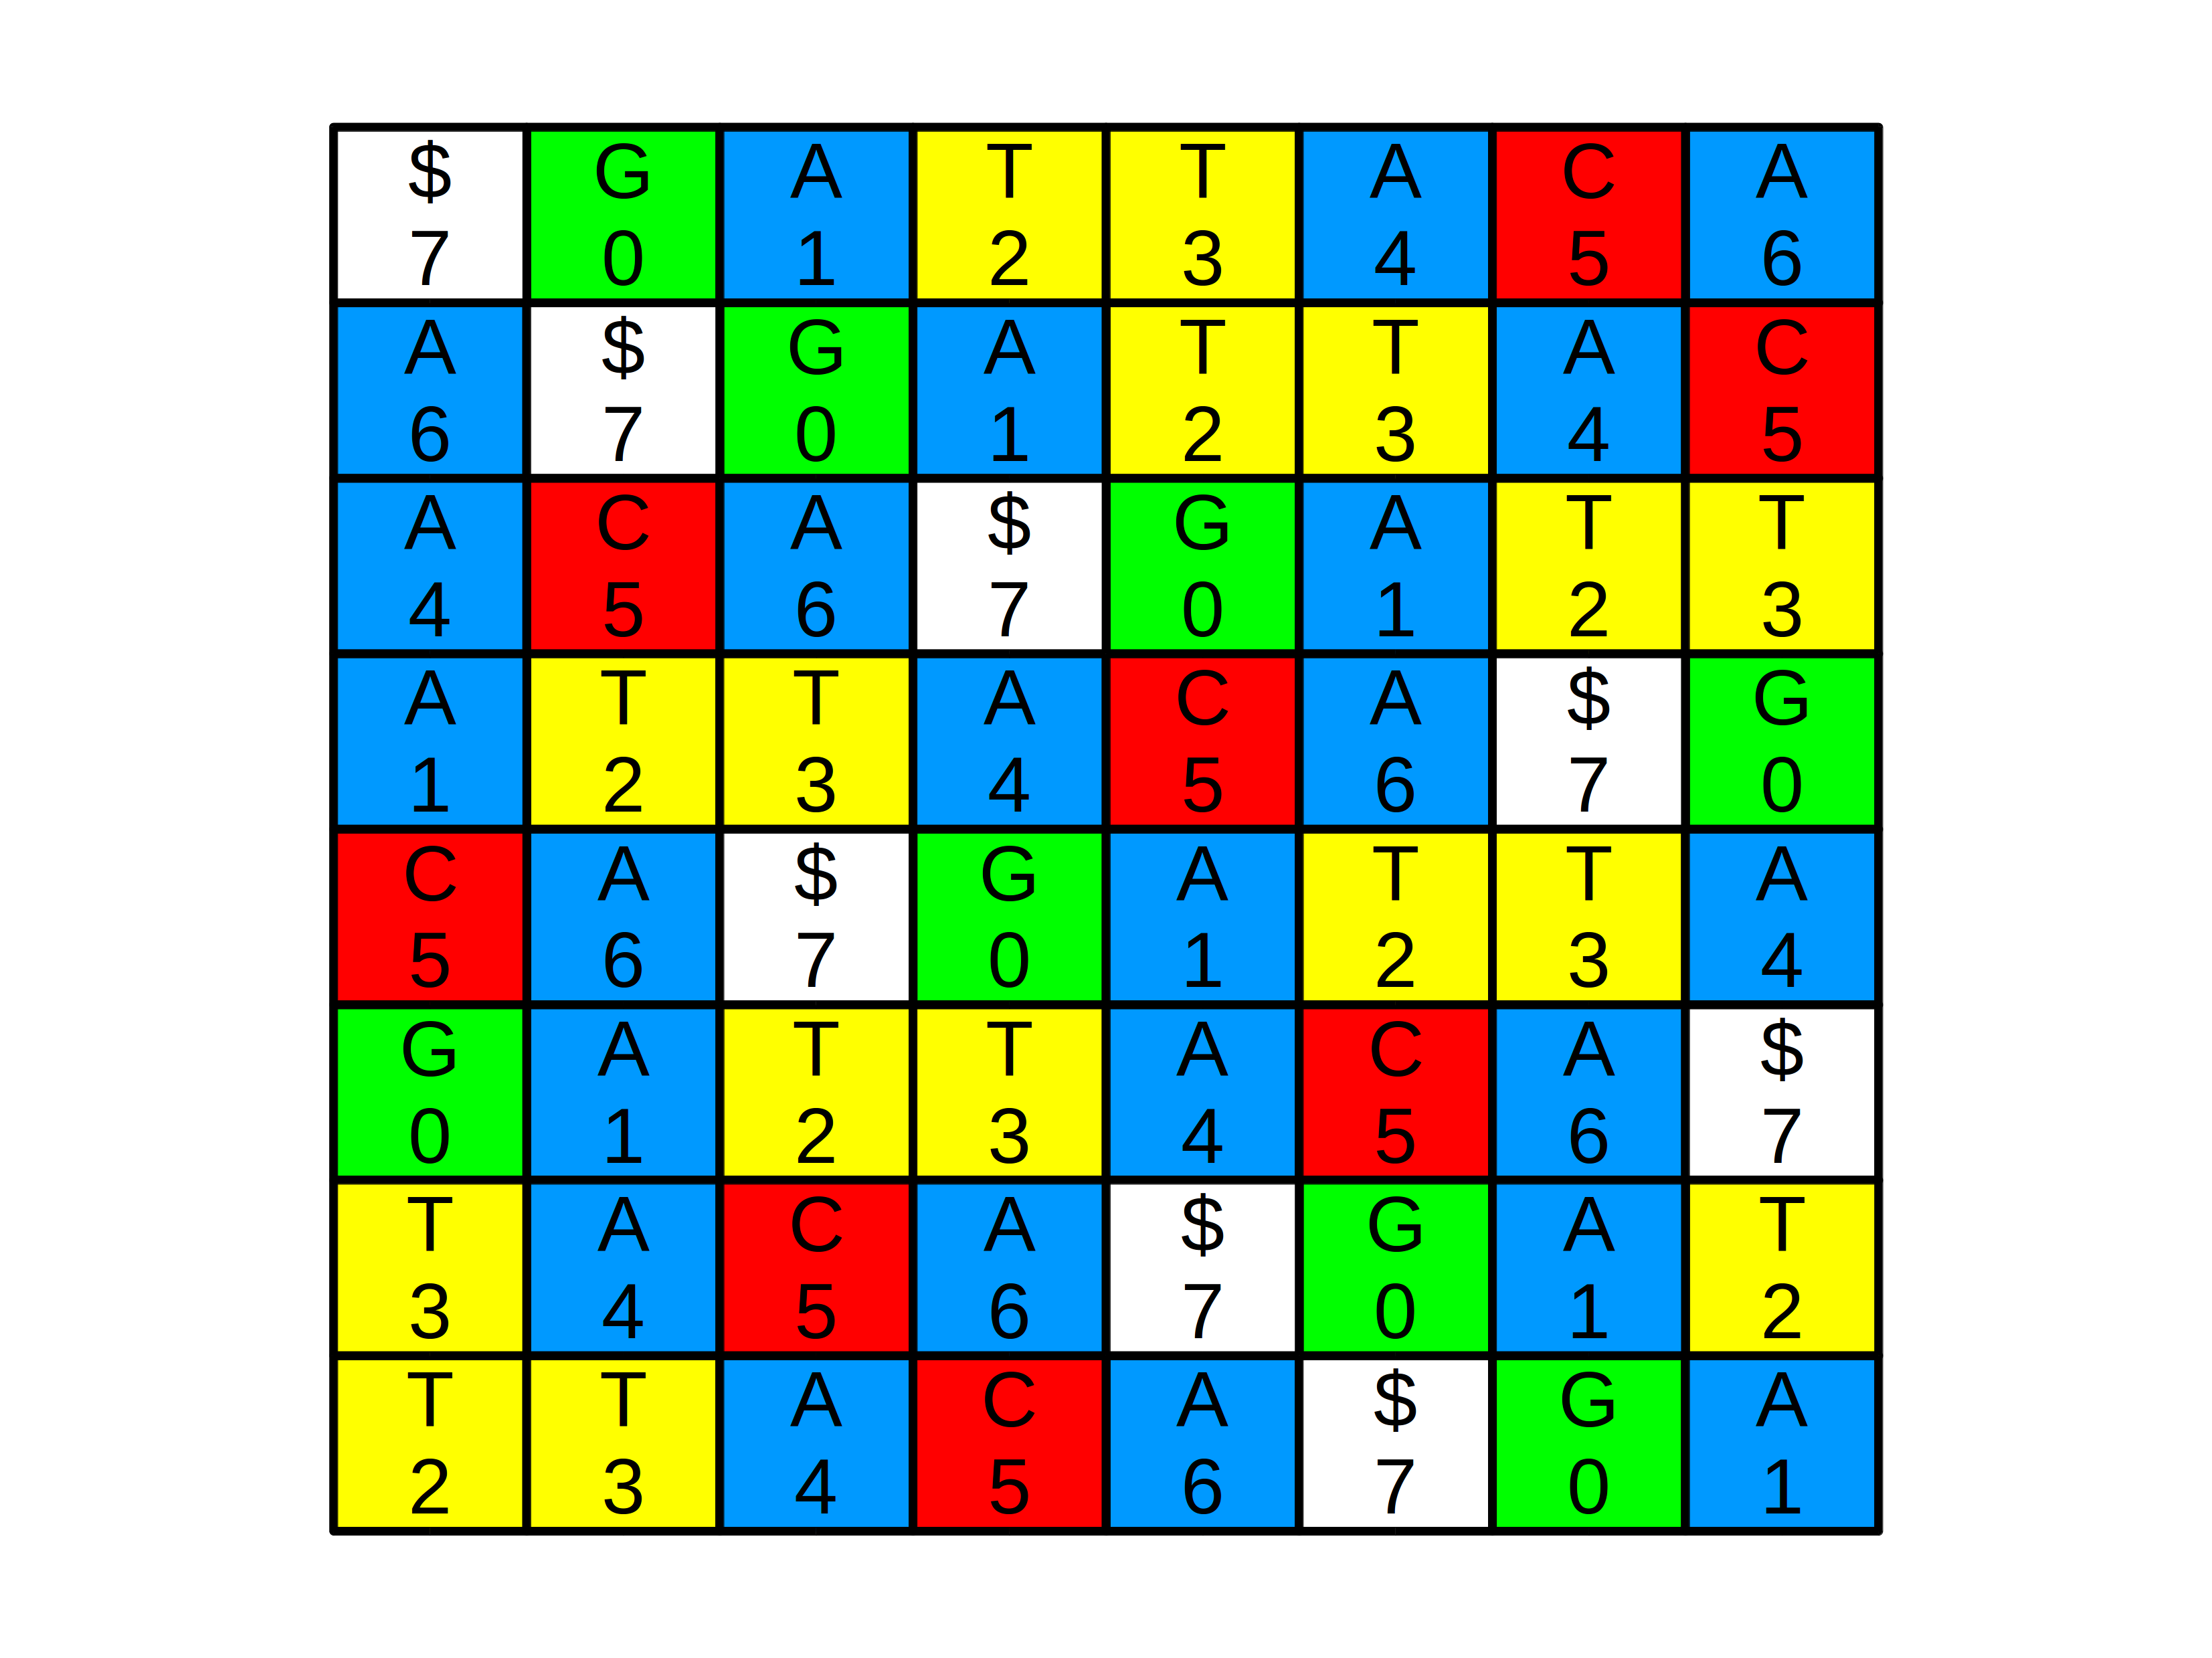
\includegraphics[width=1.0\textwidth]{figures/01_introduction/bwt.png}
    \caption[An example BWT matrix for the string ``GATTACA'']{An example BWT matrix for the string ``GATTACA''. The sentinel value ``\$'' is appended to the end of the string, all rotations of the string are calculated, and the rotations are sorted. Bases are colored according to base identity and numbered according to position in the original string. The characters in the far right column are the BWT of the original string, while the numbers in the far left column are the suffix array (represented as indices into the original string).}
    \label{fig:bwt}
\end{figure}

Note that the instances of any given character in the last column appear in the same relative order in the first column. Consider just the rows where the character in question appears in the first column. When sorting these rows, the first column is uninformative (since it is constant across all rows), and the rows are sorted lexicographically by the remaining columns in order. Rotating all the strings so the uninformative column appears last will not change the order of the other columns, and thus will not change the relative sort order of the rows we are considering. Thus the instances of the character stay in the same relative order in the last column as in the first column \cite{langmead2013introduction}.
    
\subsection{Substring Search with the Suffix Array}

The \vocab{suffix array} of a string is an array of indices into the string, sorted in the lexicographical order of the suffixes that they point to \cite{manber1993suffix}. For example, the string ``dog'' has suffixes ``dog'' at index 0, ``og'' at index 1, and ``g'' at index 2, so its suffix array would be $[0, 2, 1]$, corresponding to the suffix sort order $[\textrm{``dog''}, \textrm{``g''}, \textrm{``og''}]$. Another example suffix array is visible in the leftmost column of Figure~\ref{fig:bwt}.

Suffix arrays have some useful properties. Most importantly, all of the suffixes that start with the same substring appear in a single contiguous block \cite{ferragina2000opportunistic}. This block starts at the position corresponding to the number of occurrences of lexicographically smaller substrings of the same length \cite{ferragina2000opportunistic}. This is particularly obvious in the case of single-character substrings: all the suffixes (and, thus, all the substrings) beginning with a certain character appear in one block, coming immediately after all suffixes beginning with lexicographically smaller characters.

Suffix arrays can be used as indices to speed up substring search on the string they are derived from. Because of the block structure described above, and because every instance of a substring is at the beginning of some suffix, a simple binary search is sufficient to find any substring that is present, and a scanning up and down from one instance can pull out the entire corresponding block \cite{manber1993suffix}. Supplementing the suffix array with a \vocab{longest common prefix (LCP)} array, holding the length of the prefix shared by each pair of adjacent suffixes, can further speed up the search, by requiring only a single-character comparison (instead of a string comparison) at each search step \cite{manber1993suffix}.
    
\subsection{Searching in BWTs with the FM-index}

Constructing the BWT matrix is essentially the same task as constructing the suffix array of the string being transformed. All the rotations of the string contain the ``\$'' sentinel which is lexicographically less than all other characters. Thus the rotations are actually sorted by the portion before the ``\$'' character---that is, by the corresponding suffixes of the original string. This is the same sort used to construct the suffix array.

A BWT can be augmented with a small amount of additional information to create an FM-index (named after its inventors), which, like a suffix array, allows efficient substring search on the original string, but which also retains the compression afforded by the BWT \cite{ferragina2000opportunistic}. The FM-index is based primarily on the idea of an LF (i.e. last-first) mapping. This mapping maps each character instance in the last column of the BWT matrix to the row in which that same character instance appears in the first column. Because each BWT matrix row is a rotation of the original string, the last column of the row will contain the character instance immediately preceding the one just looked up. Thus, following the LF-mapping around the BWT from any starting position allows the characters of the original string to be enumerated from there in reverse order \cite{ferragina2000opportunistic}.

Since only the last column of the BWT matrix (i.e. the actual BWT string) is used in the algorithm, only that string needs to be stored. Furthermore, the LF-mapping can easily be calculated from the BWT string. To LF-map the character instance at a certain index in the BWT, count up the number of characters in the BWT lexicographically less than the character, and add the character instance's rank among all instances of that character. This gives the index of the LF-mapping result in the BWT.

To see why this works, recall that in a suffix array, and thus also in the BWT matrix, all the suffixes (or here rotations) that start with a given character form a contiguous block, coming just after all those beginning with smaller characters. Thus, the first calculation is to find the start of this block. And since, as shown in Subsection~\ref{subsec:bwt}, the relative order of character instances in the first column is the same as that in the last column, to find the offset of this particular character instance in that contiguous block, we merely need to find its rank among instances of the same character in the last column, which is the BWT string \cite{langmead2013introduction}.

We can now define \vocab{backward search}, a search algorithm using the BWT which processes the characters in the query string from back to front. The algorithm begins by selecting the entire BWT matrix, which is the range of suffixes that begin with the empty string. Then, for each character in the query string, from the last forwards, the algorithm extends the searched string at the front with that character. It takes the new character and finds the first and last instances of it in the BWT contained within the currently selected result range. It then LF-maps each of those instances, and takes the range between them as the new result range for the query string extended with that character. If there are no instances of the character to map, then the searched string is not found in the index \cite{ferragina2000opportunistic}.

Each row of the BWT matrix in the old range started with an instance of the old query string. Each of the rows that ended in the new query character corresponded to an instance of the old query string occurring after the new query character, and thus each implies an instance of the new, one-character-longer query string. The LF-mapping step finds the contiguous block of rows in the BWT matrix where those instances of the search string appear, the boundaries of which correspond to the first and last instances of the new character in the old BWT range (by the conservation of ordering mentioned at the end of Subsection~\ref{subsec:bwt}). Thus, such an algorithm can be used to search for substrings in a string, using the BWT of the string \cite{ferragina2000opportunistic}.

By pre-calculating some auxiliary data structures, such as a table with the start index of each character's range in the BWT matrix, and by using succinct data structures for $O(1)$ rank queries, this algorithm can be made to run in time linear in the length of the query string, and constant in the length of the index \cite{ferragina2000opportunistic}. Furthermore, using a downsampled copy of the suffix array, the location of each result in its source string can be calculated efficiently \cite{siren2009run}.

\subsection{Bidirectional DNA Search with the FMD-Index}

BWT-based indices have found many applications in genomics, mostly due to their ability to efficiently search for and identify the locations of a substrings in very large data sets---with a few modifications, this search can be extended to align reads to a reference \cite{li2014bwa}. The popular short read aligner \texttt{bwa}, for example, is built on an FM-index of the reference genome; indeed, the name stands for ``Burrows--Wheeler Aligner'' \cite{li2014bwa,li2009fast}. The ``String Graph Assembler'' \texttt{sga} also uses a BWT-based index to do its work, but in this case indexes reads themselves \cite{simpson2012efficient}.

In genomics, the strings being indexed are DNA strings, consisting of As, Gs, Cs, and Ts. These DNA strings are usually excerpts from double-stranded DNA genomes, in which, for each chromosome, two strands of DNA form a double helix. One strand runs in one direction, and the other strand runs in the other direction, with bases complemented (As and Ts swapped, and Gs and Cs swapped). It's impossible to tell whether a DNA sequencing read came from the forward strand or the reverse-complement strand until a match is found for it in a reference somewhere. Thus, many analysis problems in genomics need to consider not only some set of DNA strings but also their reverse complements.

The existence of reverse complements is accounted for in \texttt{sga} by creating two FM-indices of the input data: one index of the forward strand, and one of the reverse-complement strand \cite{simpson2012efficient}. This construction requires DNA query strings to be searched against both indices, and the results combined. However, there is a more elegant approach which allows the same search to be performed against a single index, and moreover allows bidirectional extension of the query string. This data structure, the ``FMD-index'' (the ``D'' is for ``DNA''), is simply an FM-index of both the forward and reverse strands of all input sequences, concatenated into a single data set \cite{li2012exploring}.

The FMD-index provides for double-ended search; that is, an intermediate search result can be extended with a character on either the left or right end of the query string. This works by having the FMD-index store as its intermediate result not just the single range in the BWT corresponding to BWT matrix rows that start with the query string, but also the (equally long) range for the reverse complement of the query string \cite{li2012exploring}. The first is the \vocab{forward range} and the second the \vocab{reverse range}. The fact that these two intervals will always be equally long is the key to the algorithm: because each string in the index is present as both itself and its reverse complement, any appearance of the query string has a corresponding appearance of its reverse complement. Extending the query string on the left causes the forward range to jump around in BWT coordinate space (to the regions of the BWT matrix that begin with the newly added character). However, extending on the left always causes the reverse range to cover a subrange of what it covered previously: the reverse complement of the query string gets extended on the right, and only BWT matrix rows which began with the original reverse-complement query string can possibly also begin with the longer reverse-complement query string.

The FMD-index search algorithm works as follows: When the query string is extended on the left, the forward range is updated as normal. The reverse range takes on the new interval length derived from the forward range, and a small dynamic programming problem is done over the alphabet to find its new start position. The dynamic programming problem is fairly simple because the reverse range can be partitioned into the ranges that would be selected upon left-extension with any character, ordered in lexicographic order by the reverse complement of the character. The dynamic programming simply consists of looping through the alphabet in lexicographic order by reverse complement, considering extending on each character up to the one actually being used, calculating how long the result set would be on the forward strand, and adding that in to the start of the reverse strand interval \cite{li2012exploring}. To extend a string on the right, the forward and reverse ranges are temporarily swapped, and the reverse complement of the query string is extended on its left with the reverse complement of the new base \cite{li2012exploring}.

% TODO: what if this BWT stuff can I cut, given that I'm no longer trying to use my own FMD index implementation to represent a merged-from-sequences graph?

\subsection{Previous Graph Indices}

% Improve this paragraph to actually say what is actually happening
A graph-based Human Genome Variation Map requires an efficient substring search algorithm, in order to allow sequencing reads to be efficiently aligned to the graph. Substring search in graphs is not a new idea. Many of the current approaches to this problem come at it from the perspective of trying to index a multiple sequence alignment \cite{siren2014indexing}. Two such approaches are described below.

One approach, the Generalized Compressed Suffix Array (GCSA), extends the XBW transform (itself a generalization of the BWT to trees) to ``prefix-range-sorted automata'', which include de Bruijn graphs but not general directed labeled graphs \cite{siren2014indexing}. However, the authors of that approach present only an implementation for acyclic multiple sequence alignments. The existence of nonlinear structures like polymorphic inversions, where a genomic region is forwards in some individuals but backwards in others, is not addressed, and no implementation for de Bruijn graphs is provided \cite{siren2014indexing}. Moreover, the approach presented there provides search over all possible paths through the graph in question, which is a reasonable choice for indices derived from multiple alignments, but which might backfire for graphs with short cyclic structures that could provide pathological productions for many query strings \cite{siren2014indexing}.

Another, slightly newer approach uses the concept of a ``population reference graph'', also derived from a multiple sequence alignment \cite{dilthey2015improved}. In contrast to the BWT-based indexing methods described above, the population reference graph method turns its graph representation of genomes into a Hidden Markov Model (HMM), and identifies the most likely paths through it to match the k-mer spectrum of any particular sample \cite{dilthey2015improved}. Under this method, a pair of haploid genomes are then synthesized as sample-specific references, and existing read-to-genome mapping tools are used to map sequencing reads to these references \cite{dilthey2015improved}. Unfortunately, because of the way that k-mer counts from a sample are divided up to provide input for the HMM model in different genomic regions, this method is forced to divide its HMM states into ``levels'' that it proceeds through in a fixed, sequential order. The resulting graph model is constrained to closely resemble the multiple sequence alignment it was derived from. While this method can effectively model a wide range of alternative sequences in a region, it does not appear to be able to effectively model inversions, duplications, or other more complex structures \cite{dilthey2015improved}.

% TODO: Talk about and cite GCSA2 which actually gets used

% Maybe hit the vBWT as well

\subsection{Sequence Graphs}

There are many possible representations of a genomic reference as a graph \cite{computational2016computational}, but one particularly useful model is a bidirected graph, or, when used to represent genomic data, a \vocab{sequence graph} \cite{paten2017genome}. In the sequence graph model, nodes in the graph are nucleic acid \vocab{sequences}, and each sequence has two \vocab{sides}: a ``left'' or ``start'' side and a ``right'' or ``end'' side. The sequences are connected together by \vocab{edges}, each of which has two ends that are attached to sides of nodes. The model is called ``bidirected'' because, unlike in a directed graph where each edge consists of a set of nodes and a direction (from one node to another), in a bidirected graph each edge consists of a set of nodes and two directions. The edge can still be from one node to another (in which case it connects the end side of one node to the start side of the other), but it can also be ``to`` both nodes (in which case it connects their start sides together), or ``from'' both nodes (in which case it connects their end sides together).

In a graph such as this, traversals, walks, and other graph-theoretic concepts generalize from visiting just the nodes to visiting nodes in one of two orientations: \vocab{forward} (i.e. start side to end side) or \vocab{reverse} (i.e. end side to start side). A visit to a node in the forward orientation corresponsd to the node's sequence, whereas a visit to the node in the reverse orientation corresponds to the reverse complement of its sequence. When visiting multiple nodes, it is important that the visits' orientations be consistent: if two nodes are connected by an edge from the first to the second, and you visit the first node in its forward orientation, you may next visit the second node in its forward orientation (by leaving the first node's end and arriving at the second node's start), but you may not, traversing that edge, visit the second node in its reverse orientation. In other words, the forward orientation corresponds to arriving at the start side and leaving via the end side, whereas the reverse orientation corresponds to arriving at the end side and leaving via the start side, and other combinations (such as both arriving and leaving via the start side) are not permitted.

% TODO: a figure might be nice here.

\subsection{Data Models with Protobuf}

Representing human genomic variation as a graph reference requires a data model in which to represent that graph in software. Moreover, producing an effective Human Genome Variation Map that can actually be used by other researchers requires selecting a data model that can itself be easily communicated, that can have broad software support, and that people can be persuaded to agree on.

A simple way to describe a data model and get code generated in various languages for free is to use Google's Protocol Buffers (or ``Protobuf'') library \cite{varda2008protocol}. The system provides a simple language to describe data structures, and a serialization system to allow multiple languages to read and write those data structures. The availability of libraries such as \texttt{json2pb} allows easy interoperation with any languages or tools that can consume or produce JSON. Additionally, the relative sparsity of features forces data models to be relatively simple, and the backing by a large, rich technology company helps convince people to agree on the format. Finally, the extensibility of the system allows new fields to be added to provide new features without invalidating older data sets.

Here is an example Protobuf description of a graph node in a genome graph. 

\begin{lstlisting}
// *Nodes* store sequence data.
message Node {
    string sequence = 1;   // Sequence of DNA bases represented by the Node.
    string name = 2;  // A name provides an identifier.
    int64 id = 3;     // Each Node has a unique positive nonzero ID within its Graph.
}
\end{lstlisting}
% TODO: Word wrap this

Each kind of item in the data model is referred to as a ``message'', and each field is manually assigned a unique identifying number to allow its name to be changed later while retaining backward compatibility.

Using a Protobuf-based data format for genome graphs allows for broad accessibility, without some of the disadvantages (such as large size and the necessity to write correct parsers in various languages) of bespoke text formats.

\subsection{\vg, the Variation Graph Toolkit}

% I should talk about vg, at least as it existed before I started working on it.

One collection of Probuf data models for genome graphs comes from \vg, a software suite created by Erik Garrison for working with genome graphs \cite{garrison2016vg}. In \vg, graphs are represented by a collection of nodes, each of which has an ID and a sequence, and a collection of edges, each of which connects one side (the start or end) of one node to one side of another node (which may actually be the same node, because the \vg model allows for cycles and self-loops). Each graph can also have a series of named paths associated with it, to represent how interesting things, such as the primary path of a genome assembly, or the reference version of a particular gene, fit into the graph.

The \vg suite is structured as a command-line \vg command with a variety of subcommands (\texttt{vg construct}, \texttt{vg map}, \texttt{vg view}, etc.), which are designed to be chainable into pipelines and communicate using streams of Protobuf-serialized graph data. The toolkit, The combination of the Protobuf-based serialization format, the modular architecture as a collection of subcommands, and the relatively comprehensive internal graph manipulation API make \vg and attractive option as a framework in which new genome graph algorithms can be implemented, and a useful toolkit for performing graph-based analyses.

At the time when \vg was selected as a basis for further development, it provided a data model supporting bidirected graphs, subcommand implementations for constructing, indexing, and mapping to directed acyclic graphs, and a succinct graph storage format. In part as a result of software development work undertaken as part of the present work, \vg now includes full support for working with bidirected graphs, a variant calling implementation, and a suite of unit tests.

\subsection{Copy-Number-Variable Alignments with Cactus}

When building a Human Genome Variation Map, it would be desirable to be able to incorporate variation data in the form of observed sequences, such as the European-representative MHC sequences obtained in \citet{horton2008variation}, or the many alt loci sequences provided with GRCh38 \cite{karolchik2014new}. Thus, it is necessary to have a mechanism to go from a collection of related sequences to a graph representation describing their commonalities. The \vg suite includes a tool designed to do this, \texttt{vg msga} (which stands for ``multiple sequence graph alignment''), but this tool remains under active development.

An alternative approach is to use a more mature multiple aligner tool called Cactus \cite{paten2011cactus2}. The Cactus aligner, which has been deployed in production for the production of community alignment resources \cite{howe2015wormbase}, was designed for alignment problems involving large numbers of whole genomes, and consequently understands the sorts of structural changes between genomes, such as large-scale deletions, duplications, and rearrangements, that need to be dealt with when working at those evolutionary time scales. Cactus output typically takes the form of a Hierarchical Alignment Format (HAL) file \cite{hickey2013hal,howe2015wormbase}, which uses a phylogenetic tree with internal ancestor nodes to structure information about how blocks of different genomes relate to each other. The structure formed by relationships between corresponding blocks in different genomes is quite similar to a sequence graph, with the genomes being embedded in it as paths, and so Cactus-based alignments have a natural conversion to sequence graphs.

\subsection{Reliable, Portable Cloud Computing with Toil}

% Talk about how great Toil is and how it let me do lots of the analyses in here

In order to produce a graph reference on the scale of the proposed Human Genome Variation Map, using tools like \vg that are architected as small components performing relatively simple tasks, some sort of orchestration or workflow system is necessary. This is especially true if one desires to use more than one computer in the build process; tasks need to be scheduled and code and data moved around the cluster of systems in order to perform the build. Moreover, a build process like this might require more computing resources than are required to work with the final product, and so it is desirable to be able to source those resources from on-demand cloud providers, rather than being forced to purchase them in-house.

One potential solution to this problem is Toil, a Python-based workflow development library and execution engine which is capable of composing smaller tasks into larger workflows, and of executing those workflows either on a single computer or on a cloud-based virtual cluster \cite{vivian2017toil}. Toil workflows can be written as Python scripts, which, together with Python virtual environments housing their dependencies, can be distributed to worker machines in a cloud environment. Toil nodes comunicate amongst themselves using a \vocab{job store}, which can be located on a shared filesystem or within a cloud-based distributed storage system such as Amazon's S3 or Microsoft's Azure Storage. The job store is used to keep track of which parts of the workflow have successfuly completed, and which parts have not yet executed or have failed, as well as to store files, arguments, and return values that are communicated from job to job.

Toil jobs can dynamically create and connect additional jobs in a directed acyclic dependency graph, meaning that workflows can dynamically adapt their shape to the shape of the data they are working with. Moreover, because the information required to execute each job is stored in the job store, failed jobs can be retried, and jobs suffering from bugs can be restarted with a corrected version of the workflow code, allowing problems with a large workflow to be corrected without losing all of the work done so far.

To make running on cloud providers easier, Toil provides a system to control workflow input and output, by importing data from URLs at the beginnig nof the workflow, and exporting data to URLs at the end, to eliminate the need to manually copy data to and from ephemeral cloud instances. Additionally, Toil provides a Python API for running commands through the Docker container system, allowing workflows to call command-line tools without the user having to figure out a way to get them installed on large numbers of ephemeral cloud instances. Finally, Toil integrates with Amazon Web Services to allow clusters to be automatically scaled up and down as the resource requirements of a workflow change, or as the spot market price of computing-hours rises and falls, while for Microsoft Azure Toil provides a cluster template for easy deployment in a few clicks.

\section{Research Overview}

% Maybe this is where I should talk about tying together all the cools tuff I did and why I made the decisions I made



% Chapter 2 describes the formal mapping mathematics work that I did, and is
% derived from the "Canonical, Stable, General Mapping Using Context Schemes"
% paper.
% Make floats less spacey. See <http://tex.stackexchange.com/a/26522>
\setlength{\textfloatsep}{1pt plus 1.0pt}

% Apparently we have to invent our own kinds of theorems
\newtheorem{theorem}{Theorem}
\newtheorem{lemma}{Lemma}

\chapter{Canonical, Stable, General Mapping Using Context Schemes}

\section{Abstract}
\subsection{Motivation:}
Sequence mapping is the cornerstone of modern genomics. However, most existing sequence mapping algorithms are insufficiently general.

\subsection{Results:}
We introduce context schemes: a method that allows the unambiguous recognition of a reference base in a query sequence by testing the query for substrings from an algorithmically defined set. Context schemes only map when there is a unique best mapping, and define this criterion uniformly for all reference bases. Mappings under context schemes can also be made stable, so that extension of the query string (e.g. by increasing read length) will not alter the mapping of previously mapped positions. Context schemes are general in several senses. They natively support the detection of arbitrary complex, novel rearrangements relative to the reference. They can scale over orders of magnitude in query sequence length. Finally, they are trivially extensible to more complex reference structures, such as graphs, that incorporate additional variation.
We demonstrate empirically the existence of high performance context schemes, and present efficient context scheme mapping algorithms.

\subsection{Availability and Implementation:}
The software test framework created for this work is available from \url{https://registry.hub.docker.com/u/adamnovak/sequence-graphs/}.

\subsection{Contact:} \href{benedict@soe.ucsc.edu}{benedict@soe.ucsc.edu}
\subsection{Supplementary Information:} Six supplementary figures and one supplementary section are available with the online version of this article.

\section{Introduction}

%%Benedict's proposed introduction - the reference numbers are all wrong.

Many tools and algorithms exist for mapping reads to a reference genome \citep{li2010fast,langmead2009ultrafast,harris2007improved}. These tools are based on the idea of scoring local alignments between a query string and a reference according to some set of match, mismatch, and gap scoring parameters, and then finding local alignments with maximal or near-maximal scores. Seed-and-extend approaches coupled with memory efficient substring indexes or hashing schemes have been highly successful in heuristically accelerating this search process \citep{dobin2013star,li2010fast,langmead2009ultrafast}. 

The core problem with read mapping is ambiguity. There is often no single best place that a read maps, especially in the case of recent duplication within the reference genome. The precise base-level alignment of the read to a given location in the reference is also often ambiguous. To mitigate this, each mapped read is given a mapping quality, a per read score that indicates how likely the mapping was generated erroneously \citep{li2008mapping}. Quantifying this uncertainty is a reasonable approach for many applications, but even then the uncertainty can be difficult to accommodate downstream.

The difficulty of mapping a read to a reference motivates a consideration of its necessity. Recently, alignment-free methods of variant calling through substring detection have garnered significant interest \citep{dilthey2014improved}. The basic idea is not new; the dbSNP database has long provided, for each point variant in the database, a flanking nucleotide string that indicates the DNA context in which the variation was isolated \citep{sherry2001dbsnp}. In principle such a system of variant identification sidesteps the limitations of score based alignment, and can be used to canonically detect variations. However, in practice, insufficient rigor in defining the substrings to detect, and a failure to account for other variation near identified point mutations have limited the approach's usefulness. Here we formalize and extend this core idea; we propose using multiple, algorithmically defined context strings to canonically identify the presence of each base within a reference genome (potentially paving the way for high-specificity, alignment-free variant calling) and evaluate the performance of such a method in practice. 

%Cut for brevity
%In its simplest form, each reference base is labeled by a ``context string'' that, when detected in a query sample, is sufficient to unambiguously identify the base’s presence. To account for the randomly placed boundaries of short sequencing reads, which would often inconveniently truncate any single context string for a reference base at one end or the other, and to accommodate other nearby variation, we generalize the notion from a single context string per base to a set of such strings per base. When such a system is applied across a reference genome it defines a mapping scheme; we call this a ``context-driven'' mapping scheme. We first define context-driven mapping schemes in general, then give a specific, useful scheme and develop associated algorithms for its implementation. Finally we demonstrate empirically its practicality for the mapping of assembled sequences, as well as individual reads.

%%End of benedict intro


% We want to do variant calling

% People tried to do variant calling without mapping.

% It turns out that that's hard

% So we present a new mapping method inspired by these attempts at reference-free variant calling


%Everybody in genomics wants to call variants. We already have an idea of what human genomes look like in general; when an individual is sequenced, the primary concern is how that individual differs from the human reference genome. This is usually determined by aligning sequencing reads from the individual against the reference genome, and explaining differences between the reads and the reference by invoking variants in the individual. However, read mapping is a complex and slow process; it only works as well as it does because of the thousands of hours of work people have spent on heuristic acceleration and optimization \citep{dobin2013star,li2010fast,langmead2009ultrafast}.

%The difficulty of mapping a read to a reference motivates a critical consideration of its necessity. Some approaches to variant calling rely instead on the identification of substrings within collections of reads in order to ascertain the presence or absence of genomic variants \citep{dilthey2014improved}%REF-DURBIN? POSSIBLY
% Citing Gil's HMM preprint thing
%. The dbSNP database caters to this view by attaching to each point variant in the database upstream and downstream flanking nucleotide strings that indicate the DNA context in which the variation was isolated \citep{sherry2001dbsnp}. In principle, this would allow dbSNP variants to be identified in a reference-free way. However, insufficient rigor in defining appropriate context strings, and a failure to account for other variation near the identified point mutation has limited the use of these sequences in practice.  

%%Overview of method, which combines notion of context sequences

%What is needed is a middle ground between traditional read to reference genome alignment and reference-free methods of variant detection. We would like to preserve the idea of a space in which variants exist, while phrasing uses of read data in terms of simple and formally tractable substring operations. 

%Here we propose using context strings to canonically identify the presence of each base within a reference genome. We build on the idea of labeling each reference base with a ``context string'' that, when detected in a query sample, is sufficient to unambiguously identify the base's presence. To account for the randomly placed boundaries of short sequencing reads, which would often inconveniently truncate any single context string for a reference base at one end or the other, and to accommodate other nearby variation, we generalize the notion from a single context string per base to a set of such strings per base. When such a system is applied across a reference genome it defines a mapping scheme; we call this a ``context-driven'' mapping scheme.

%We first define context-driven mapping schemes in general, then give a specific, useful scheme and develop associated algorithms for its implementation. Finally, we empirically demonstrate our method's practicality for the mapping of assembled sequences, as well as individual reads.


\section{Methods}

%Define genome, reference genome and input sequence

%Definition of a mapping function

%%Mention how we deal with multi-mapping (point at hierarchy stuff in other paper).

%Definition of a context scheme

%Properties of a context scheme
%%Stability
%%Non-linearity
%%Extension to graphs
%%Uniqueness/functional mapping

Throughout we make use of \vocab{DNA strings}, which are finite strings over the alphabet of \vocab{DNA bases} $\left\{\mathrm{A}, \mathrm{C}, \mathrm{G}, \mathrm{T}\right\}$. 
%Removing for brevity. This is unnecessary in my opinion.
%A DNA string $x$ has \vocab{elements} $1$ through $n$; each element $i$ in $x$ has a \vocab{base} $x_i$ that appears in the string at index $i$. 
A DNA string $x$ has a \vocab{reverse complement} $x^*$, which is the reverse of $x$ with each DNA base replaced with its complement; $\mathrm{A}$ and $\mathrm{T}$ are complements of each other, as are $\mathrm{G}$ and $\mathrm{C}$. 

\subsection{Mapping}
A \vocab{reference (genome)} $G$ is a set of DNA strings and an index set of the elements of these strings, each member of which is called a \vocab{position}. Each position $p$ uniquely identifies an element $b(p)$ of a string in $G$. This allows us to unambiguously discuss the ``positions'' in that set of DNA strings, rather than ``bases'' or ``characters'', which could be interpreted as the four DNA bases themselves.

 We define the problem of mapping a \vocab{query} DNA string $x=(x_i)_{i=1}^n$ to a reference $G$. 
A \vocab{mapping scheme} is a function that takes $x$ and $G$ and, for each query element $i$ of $x$, either returns a position in $G$, declaring the query element $i$ to be \vocab{mapped} to that position in $G$, or declares the query element to be \vocab{unmapped} in $G$. For the scheme to map a query element to a position $p$ in $G$, $b(p)$ must either be $x_i$ (in which case that query element is \vocab{forward mapped}), or ${x_i}^*$ (in which case that query element is \vocab{reverse mapped}). 

\subsection{Contexts}
A \vocab{context} is a tuple $(L, B, R)$, where $L$ is a DNA string called the \vocab{left part}, $B$ the base, and $R$ is a DNA string called the \vocab{right part}. The string $LBR$ is the \vocab{context string} of the context $(L, B, R)$. The context distinguishes $B$ from the rest of the context string, so that when the context is found to occur in a query string, it is clear which character in the query string (i.e. the one corresponding to $B$) has been recognized.
For an element $i$ in a DNA string $x$ a context $(L, B, R)$ is called a \vocab{natural context} if $B=x_i$,  $L$ is a (possibly empty) suffix of $(x_j)_{j=1}^{i-1}$ and $R$ is a (possibly empty) prefix of $(x_j)_{j=i+1}^n$. Some example natural contexts are visible in Supplementary Figure~S1. % We need this since we are going to want to assign contexts with mismatches later that don't actually appear in the strings in the reference


\subsubsection{Context Generality}
A context $c_1 = (L_1, B_1, R_1)$ is \vocab{forward more general} than a context $c_2 = (L_2, B_2, R_2)$ if $L_1$ is a suffix of $L_2$, $B_1 = B_2$, and $R_1$ is a prefix of $R_2$. That is, if you turned the two contexts into strings with their bases marked as special characters, the more general context would be a substring of the \vocab{less general} context. Note that a context is forward more general than itself. A context $c_1$ is \vocab{reverse more general} than a context $c_2$ if $c_1$ is forward more general than the reverse complement of $c_2$, which is $c_2^* = (R_2^*, B_2^*, L_2^*)$. We define a context $c_1$ to be generically \vocab{more general} than context $c_2$ if it is either forward more general or reverse more general than $c_2$. 
%Cut for brevity
%We use the term \vocab{(forward/reverse) less general} for the inverse relation.

\subsection{Context-Driven Mapping}
It is possible to define a mapping scheme for a query string $x$ to a reference $G$ in terms of contexts for positions in the reference. Such a mapping scheme makes use of a context assignment.

\subsubsection{Context Assignment}
A \vocab{context assignment} assigns each position in a reference a nonempty \vocab{context set}, such that all contexts in the set have the same base as the position, and no context in one position's set is more general than any context in any other position's set (Figure \ref{fig:contextSets}). This second property of context assignments is called \vocab{nonredundancy}.  
%Cut for brevity
%Note, however, that it is possible for two contexts from different context sets, neither of which is more general than the other, to both be more general than some context in which a query base is observed; nonredundancy does not guarantee nonambiguity.

\subsubsection{Matching}
An element $i$ in a query string $x$ is said to \vocab{match} a context $c = (L, B, R)$ if the query, when partitioned into the context $((x_j)_{j=1}^{i-1}, x_i, (x_j)_{j=i+1}^n)$, is less general than $c$. Note that this encompasses both forward less general (in which case element $i$ \vocab{forward matches} the context) and reverse less general (in which case element $i$ \vocab{reverse matches} the context). When the context is in the context set of a reference position, the element \vocab{matches} the position \vocab{on} the context. 

%Cut for brevity
%Elements can also match positions. An element $i$ in a query DNA string is said to \vocab{match} a position $p$ in a reference under a context assignment $C$ if element $i$ matches some context in $p$'s context set assigned by $C$. If $i$ forward matches the context this is \vocab{forward matching}, and if $i$ reverse matches the context this is \vocab{reverse matching}. (Note that due to the requirements on the base of a context it is impossible to both forward match and reverse match the same position.) Element $i$ is said to \vocab{match on} the context.

\subsubsection{Context-Driven Mapping Schemes}
% This paragraph starts on the same line as the subsubsection title and wants to escape the margins.
\begin{sloppypar}
A \vocab{context-driven mapping scheme} is a mapping scheme which, for query $x$ and reference $G$ with context assignment $C$, maps each element $i$ in $x$ to the unique position in $G$ which it matches under $C$, or leaves $i$ unmapped when no such position exists. An element remains unmapped when it does not match any context of a reference position, or when it matches contexts of two or more positions; in the latter case we say it \vocab{discordantly matches}, an example of which is visible in Supplementary Figure~S2.
\end{sloppypar}


Under a (nonredundant) context assignment, each position $p$ in the reference can be mapped to, because for each context $(L, B, R)$ of $p$ the context string $LBR$ matches $p$ on that context. The nonredundancy requirement ensures this matching is not discordant: no context more general than $(L, B, R)$ can be in the context set of any other position in the reference.

\subsubsection{Stability}
An \vocab{extension} of a DNA string $x$ is a DNA string that contains $x$ as a substring.  
An element $k$ in an extension $x'$ of $x$ is a \vocab{partner} of an element $i$ in $x$  if the context $((x_j)_{j=1}^{i-1}, x_i, (x_j)_{j=i+1}^n)$ is more general than $((x'_j)_{j=1}^{k-1}, x'_k, (x'_j)_{j=k+1})$.

A mapping scheme is \vocab{weakly stable} 
if for each element $i$ in each possible query string $x$, if $i$ is mapped to a position $p$ in the reference, its partners in all extensions of $x$ will map to $p$ or be unmapped.
Weak stability is desirable because it guarantees that an element in a query cannot change its mapping to a different position under extension---the mapping scheme never has to admit that it mistook one reference position for another when presented with more information. Unlike score based mapping procedures, which are generally not weakly stable, all context-driven mapping schemes are weakly stable, because for any mapped element $i$, the partners of $i$ in an extension of the query string can only either map to the same position $p$, or be discordantly matched and therefore unmapped. This is because these partners have all the natural contexts of $i$, and therefore must match on a context in the context set of $p$, but may additionally match on the context of a different position in the reference and therefore discordantly match.
%\subsubsection{Stable Context-Drive Mapping Schemes}

A mapping scheme is \vocab{stable} 
if for each element $i$ in each possible query string $x$, if $i$ is mapped to a position $p$ in the reference, its partners in all extensions of $x$ will map to $p$. Stability is naturally a more desirable property than weak stability, as it restricts mapping to individual positions aligned with high certainty.
%, because once mapped an element in a query string remains mapped to the same position under extension.
By the argument above, some context-driven mapping schemes are only weakly stable. A \vocab{stable context-driven mapping scheme} is equivalent to a context-driven mapping scheme that additionally makes an element of a query string unmapped if a partner element in any extension of the query would discordantly match. 
%This is unnecessary.
%Although it might seem obvious, it is important to note that a ``stable context-driven mapping scheme'' is stable as defined above.

\begin{figure}
  \begin{minipage}{0.5\linewidth}
  \centering
  \begin{tabular}{rcl}
  \multicolumn{3}{c}{Contexts for position $P_1$} \\ \hline
  $(L,$ & $b,$ & $R)$ \\ 
  \texttt{TGTCGC} & \texttt{C} & \texttt{CAAGCA} \\ 
  \texttt{TG\textbf{G}CGC} & \texttt{C} & \texttt{CAAGCA} \\ 
  \texttt{TGTCGC} & \texttt{C} & \texttt{CA\textbf{C}A} \\ 
  \end{tabular}
  \end{minipage}%
  \begin{minipage}{0.5\linewidth}
  \centering
  \begin{tabular}{rcl}
  \multicolumn{3}{c}{Contexts for position $P_2$} \\ \hline
  $(L,$ & $b,$ & $R)$ \\ 
  \texttt{ACGAC} & \texttt{C} & \texttt{CCAG} \\ 
  \texttt{CGAC} & \texttt{C} & \texttt{C\textbf{T}} \\ 
  \texttt{ACGAC} & \texttt{C} & \texttt{CCA\textbf{T}G} \\
  \end{tabular}
  \end{minipage}

  \caption{Example of two nonredundant context sets. Substitutions relative to the first context in each set are in bold. If the context $(L, B, R) = \texttt{C}, \texttt{C}, \texttt{C}$ were added to either set, it would make the context assignment redundant, as it is more general than contexts that already occur in both sets.}
  \label{fig:contextSets}
\end{figure}

\subsection{The Natural Context-Driven Mapping Scheme}

%%Point to earlier paper for previous schemes.
In our earlier paper \citep{paten2014mapping} we discussed a number of different context assignments, including fixed $k$-mer approaches. Here we focus on a new scheme that is easy to reason about and which performed the best in our preliminary empirical tests (Supplementary Figure~S3).

%The Natural mapping schemes

The \vocab{natural context assignment} assigns to each position in the reference the subset of its natural contexts that are not natural contexts of any other position in the reference. It is trivially nonredundant.
%Need a figure to illustrate this
% Do we really?
The \vocab{natural (context-driven mapping) scheme}, which uses the natural context assignment, has an intuitive interpretation: an element $i$ of a query string is mapped to a position $p$ of the reference when all natural contexts of $i$ with context strings unique in the reference are are assigned to $p$.

%Algorithms for natural context schemes
%%%Define max unique substrings and inchworm recursion, keep it very brief.
\subsubsection{Overview of Algorithms}
The natural context scheme is also simple to implement. For a reference and query, a \vocab{maximum unique match (MUM)} is a maximum length substring of the query present once in the reference. % TODO: Does this adequately exclude the idea that we can take a MUM that has a longer version somewhere else in the query and declare it not a MUM?
Our definition of a MUM differs from that used by tools like MUMmer \citep{delcher1999alignment} in that it is nonsymmetric; we allow a MUM to have multiple \vocab{MUM instances} in the query, each of which is a MUM and an interval of the query corresponding to a location of the substring. For a query $x$ of length $n$ there are at most $n$ MUM instances, since two cannot start at the same place. Each MUM instance that contains a given element $i$ can be described as a natural context string of $i$: $(x_j)^{i-1}x_i(x_j)_{i+1}$. Under the natural context assignment, the context of each such MUM-derived context string matches exactly one reference position. %Each element $i$ in $x$ can be contained in no more (and probably far fewer) than $n$ MUM instances. 


Using a suffix tree with suffix links of the strings in a reference (which can be constructed in time linear in the sum of the length of the reference strings), or a related substring index data structure, it is possible to find the set of MUM instances for a query string ordered by ascending start element in $O(n)$ time. These data structures all provide two $O(1)$ operations, \vocab{extend} and \vocab{retract}, which, given a search result set for some search string, can produce the result set for a search string one character longer or shorter, respectively. Employing these operations to find all MUMs in order by ascending query start position is straightforward. Starting with the empty string, extend the search string on its right end with successive characters from the query string until such an extension would produce a search result set with no results (or until the query string is depleted). If at that point there is one result in the result set, and at least one extension has happened since the last retraction, then a MUM has been found. Next, retract a single character from the left end of the search string, and go back to extending with the remaining unused query string characters. Repeat the whole process until the query string is depleted.


%Cut for brevity (is redundant to above) When no more extends can be performed without losing the single unique result, the query substring represented by the search string is unique and maximal on the right. If, additionally, at least one extend has happened since the last retract, then this match is also maximal on the left. (If it was not, the most recent extend would have been performed before the most recent retract.)  

Since each successful extend operation consumes a character from the query string, no more than $O(n)$ extend operations can ever be performed. Since each retract operation moves the left end of the search string to the right in the query, no more than $O(n)$ retract operations can be performed. And since each unsuccessful extend operation (which would produce an empty result set) is followed by a retract operation, no more than $O(n)$ of those can happen either. Thus the entire algorithm is $O(n)$. 

Once the MUM instances have been found, it is necessary to identify the query elements that occur in exactly one MUM and therefore can be mapped under the natural scheme. (If an element is contained in two or more MUM instances then it must be discordantly mapped, because each must define a context that matches the element to a distinct position.) Given the MUM instances ordered by ascending query start element, it can be determined for all elements if each is in one, zero or multiple MUM instances, by a single traversal of the ordered MUM instances taking $O(n)$ time. We can therefore determine in $O(n)$ which elements in a query string are mapped. The combined time to map all the elements in a new query string given an existing reference substring index data structure of the type discussed is therefore $O(n)$.

\subsection{The $\alpha$-$\beta$-Natural Context-Driven Mapping Scheme}

%Introduce \alpha hamming separation of context strings
Under the natural context assignment, for each (by definition minimally unique) reference context string, there must exist another reference substring that is an edit distance of one from it.  Therefore, while the natural context assignment ensures each context identifies a single position in the reference, a single substitution, insertion or deletion in a query substring could result in a change in mapping. To avoid this, we now define a more robust scheme.

Throughout, we use the Levenshtein edit distance, in which a single character replacement, insertion, or deletion is worth one. This choice of edit distance metric makes reasoning about the behavior of our algorithms simpler, but they could potentially be extended to other metrics tailored to different sequence data sources.

%First we introduce the concept of \vocab{irreconcilable} reference substrings, which are reference substrings for which no minimal edit distance alignment exists that pairs up all bases with the same positions.

%For a given context $c$, we define \vocab{$\alpha$-separation} as the minimum edit distance $\alpha$ between $c$'s context string and any other irreconcilable substring in the reference. A context assignment that enforces a minimum $\alpha$-separation between contexts in different context sets can be more robust against spurious mappings due to edits in the query.

For a pair of overlapping substrings $(x_j)$, $(x_k)$ of a string $x$, we call elements in either substring not contained within the intersection of their intervals on $x$ \vocab{separate}.  For two substrings within the reference (not necessarily overlapping or even in the same reference string) we can similarly talk about their number of separate elements. For a given reference substring, the \vocab{$\alpha$-separation} is the minimum edit distance $\alpha$ between it and any other substring in the reference with a number of separate elements greater than its edit distance from the original substring. For a given natural context of a reference position, its $\alpha$-separation is the $\alpha$-separation of its context string.

Having a minimum $\alpha$-separation for contexts in a natural context scheme makes mappings more stable in the face of edits to the query. Specifically, it ensures that the number of edits required to transform the context of one position into the context of another is at least $\alpha$, for positions whose context strings have more than $\alpha$ separate elements. %For positions whose context strings have $\alpha$ or fewer separate elements, $\alpha$-separation tells us nothing.
When two reference substrings with $\alpha$ edit distance have exactly $\alpha$ separate elements (it is easy to verify they can not have fewer than $\alpha$) then there exists a minimum edit-distance alignment of the two substrings that only aligns together bases from each substring with the same reference positions, and the $\alpha$ edit distance is therefore trivially realizable as the removal of a prefix from one substring and a suffix from the other. However, it is also possible that two substrings with $\alpha$ edit distance and $\alpha$ separate elements could have other minimum edit distance alignments that would result in different mappings. Therefore, enforcing $\alpha$-separation on a context assignment does not absolutely prevent mismappings produced by fewer than $\alpha$ edits---however, such mismappings would have to be relatively localized on the reference. 

%(When two reference substrings with $\alpha$ edit distance have $\alpha$ separate elements (it is easy to verify they can not have fewer than $\alpha$) then there exists a minimum edit-distance alignment of the two substrings that only aligns together bases from each substring with the same reference positions, and the $\alpha$ edit distance is therefore trivially reconcilable as the removal of a prefix from one substring and a suffix from the other). Similarly, for a given natural context of a reference position, its $\alpha$-separation is the $\alpha$-separation of its context string. A context assignment that enforces a minimum $\alpha$-separation for contexts can be more robust against spurious mappings due to edits in the query that would result in different mapping.




%Introduce \beta hamming separation of the natural and query contexts.
Similarly, the natural context assignment is intolerant to edits between the query string and context strings of positions in the reference to which we might like query elements to map. To mitigate this issue, for a given context $(L,B,R)$ and element $i$ in DNA sequence $x$ we define \vocab{$\beta$-tolerance}: if $x_i = B$, $\beta$ is the minimum edit distance between the context string $LBR$ and a natural context string of $i$. If $x_i \not= B$ then $\beta=\infty$. 
%I think this is unnecessary
%(We can also extend this definition to talk about the $\beta$-closeness of two contexts, or a context and a reference position.)
Hence for a position in the reference $p$, a $\beta$-tolerant context $(L, B, R)$ is a context such that $b(p) = B$ and $LBR$ is within $\beta$ edits from a natural context string of $p$. 
The \vocab{$\alpha$-$\beta$-natural context assignment} assigns each position in the reference a context set containing the minimal length contexts that are at least $\alpha$-separated, and at most $\beta$-tolerant from it. 
%I *think* the following statement is true - it is important to be sure!! V. nice if true.
% beta < alpha is all you really need.
% To be assigned to a position, a context must be edit distance alpha from all other positions' natural contexts.
% Extending a context cannot decrease the minimal distance between it and any context in the set of natural contexts of a position.
% So if a context is edit distance alpha from a position's natural context, no less general context can be less than edit distance alpha from that position's natural contexts
% So if a position is alpha-separated, neither it nor any less general context can be beta-close to any other position, unless beta >= alpha.
% So if beta < alpha, no context that was beta-close enough to be assigned to one position can have a more general context that was alpha-separated enough to be assigned to another.
It can be verified that as long as $\alpha$ is greater than or equal to one and $\beta$ is less than $\alpha/2$ then the context assignment is nonredundant and therefore valid.
The $\alpha$-$\beta$-natural context assignment ensures all admitted contexts are both $\alpha$-separated (and therefore unlikely to be matched by chance, requiring $\alpha$ misleading edits to coincide), and at most $\beta$-tolerant (and therefore tolerant of up to $\beta$ edits obscuring the true reference position). The natural context-driven mapping scheme is a special case of the \vocab{$\alpha$-$\beta$-natural (context-driven mapping) scheme} when both $\alpha$ and $\beta$ equal 0. (A possible extension would be a context scheme in which the $\alpha$-separation and $\beta$-tolerance required to admit contexts depended on the context length, but this would make the parametrization of the context scheme quite complex, and so is not explored here.)

\subsubsection{Overview of Heuristic Algorithms for the $\alpha$-$\beta$-Natural Context-Driven Mapping Scheme}

%%Give heuristic algorithms for \alpha and \gamma natural context schemes
Unfortunately, algorithms built on efficient substring indexes to implement the $\alpha$-$\beta$-natural scheme require tracking a number of potential matches that is exponential in both $\alpha$ and $\beta$ parameters. Instead we pursue an algorithm that heuristically approximates this scheme. A full description of this algorithm is available in Supplementary Section~S1; the basic idea, inspired by existing seed-and-extend hashtable methods and chaining methods like BWA-MEM, is to chain exact matches separated by mismatching gaps, until a sufficient $\alpha$-separation is obtained \citep{li2010survey, li2013aligning}.

For a reference, a \vocab{minimal unique substring (MUS)} is a shortest length substring that appears once in that reference. 
Two MUSes are disjoint if they do not overlap. We define $\alpha'$ as the maximum number of disjoint MUSes within a context string. It is easy to verify that $\alpha'$ is a lower bound on $\alpha$. Intuitively, each disjoint MUS would need to be disrupted by a distinct edit.

The heuristic algorithm attempts to chain together MUMs to accumulate at least $\alpha'$ disjoint MUSes, without requiring more than $\beta'$ edits in the \vocab{interstitial substrings} between the MUMs. This creates \vocab{$\beta'$-synteny blocks}, as depicted in Figure~\ref{fig:model}, which are maximal sequences of MUMs that agree in order and orientation, and which have $\beta'$ or fewer edits between the strings they mark out in the reference and the query. If a $\beta'$-synteny block can be created that has at least $\alpha'$ disjoint MUMs (and is thus $\alpha'$-separated), the MUM instances it contains are used as in the natural mapping scheme above, to define contexts for the involved reference positions.

This heuristic algorithm, as demonstrated in Supplementary Section~S1, finds contexts of reference positions in the query string that are at least $\alpha'$-separated, and at most $\beta'$-tolerant, and takes $O(\beta'^2n)$ time to map the query string, given the previously described substring index structure for the reference. Provided $\alpha^\prime < \beta^\prime$, this context scheme is nonredundant. The contexts found (and thus the matchings made) by this heuristic scheme are a subset of those that would be produced by the exact algorithm, although the same is not always true of the resulting mappings. A more thorough, empirical comparison of this heuristic scheme to an implementation of the exact scheme is left as future work, primarily due to the above-mentioned computational difficulty inherent in nontrivial exact $\beta$ values.

\begin{figure}
\centering
  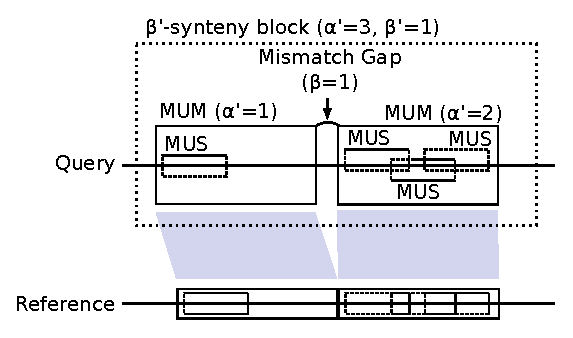
\includegraphics[width=1.0\columnwidth]{figures/02_contextschemes/MUMs.eps}
  \caption{Diagram of a $\beta^\prime$-synteny block for the $\alpha^\prime$-$\beta^\prime$-natural context scheme, composed of two MUMs.}
  \label{fig:model}
\end{figure}

\subsection{Credit}
%Introduce credit schemes

It is common to find some elements in a query string $x$ which are unmapped, and cannot be mapped on any extension of $x$, yet are intuitively recognizable as corresponding to reference positions. This often happens if bases are between two MUMs but are not part of any MUM themselves, or if they were part of a MUM between two other MUMs that cannot join a sufficiently $\alpha'$-separated $\beta'$-synteny block. In these cases, to create a scheme that maps more elements of the query,  we can augment our context assignments with additional contexts that allow such bases to map \vocab{on credit}, based on the mappings of the bases on either side. The particular credit method used here looks at the nearest mapped base on either side of a gap in mapping, and matches up elements with the correct bases with respect to their implied positions in the reference, allowing at most one mismatch. Previously unmapped elements that are matched to exactly one reference position will be mapped on credit, while elements that are matched to zero or two positions will not map.

Since only elements that did not already match, and which could not possibly match on any extension of the query, are mapped in this way, the addition of credit does not interfere with the nonredundancy of a context assignment or the stability of a context-driven mapping scheme.

% TODO: Make sure we are properly blacklisting bases from credit if they didn't map due to conflict, or are in MUMs too close to the ends.

\section{Results}
\label{sec:results}

%%Describe setup with the MHC

In order to test the utility of the theoretical constructs described here, a series of software tests were created in order to evaluate the mappings produced by the $\alpha$-$\beta$-natural scheme described above. Mapping accuracy was evaluated for both error-corrected long sequences and error-prone short sequences.

\subsection{Mapping MHC Alt Loci}

To evaluate the performance of the new mapping algorithms proposed here a long-sequence mapping task was defined. The human genome has, on chromosome 6, a region of approximately 5 megabases known as the \vocab{major histocompatibility complex (MHC)}, rich in antigen presentation genes vital to the function of the immune system \citep{the1999complete}.
The region is prone to complex rearrangement, is well-supplied with both coding and noncoding sequence, and exhibits extreme regional variation in the polymorphism rate along its span \citep{the1999complete}. As one of the most complex and difficult regions of the genome, it provides a good testbed for methods designed to deal with difficult structural variation. To better represent the complexity of this region, the Genome Reference Consortium (GRC)'s current human reference assembly (GRCh38) contains seven full-length MHC \vocab{alt loci}, each of which serves as a different alternate reference for the region \citep{church2011modernizing}. These alt loci come with official alignments to the chromosome 6 primary sequence, which are part of GRCh38 and were generated using the NGAligner tool and limited manual curation \citep{schneider2013genome,schneider2015grc}.

Each mapping scheme under test took the MHC alt loci (GI568335879, GI568335954, GI568335976, GI568335986, GI568335989, GI568335992, and GI568335994), and mapped each to the GRCh38 \vocab{primary path} region, which actually appears in the ``chr6'' FASTA record. The resulting alignments were compared against the official GRC alignments distributed with GRCh38, with the caveat that aligned, mismatched bases in the GRC alignments were de-aligned to ensure a fair comparison, as the mapping schemes being evaluated were not permitted to align mismatching bases together. (Allowing mismatching bases in the GRC alignments to align made no perceptible difference in any figure, and was not pursued further.) The standard information retrieval metrics of precision and recall against the GRC alignments were calculated using \texttt{mafComparator}, and can be seen in Figure~\ref{fig:mhcprecisionrecall} \citep{earl2014alignathon}. Overall coverage (the fraction of bases of an alt locus aligned to the reference), and the frequency and size of rearrangement events implied by the alignments, were also calculated, and are visible in Figure~\ref{fig:mhccoverage} and Figure~\ref{fig:rearrangements}, respectively.

%Coverage
%Min/max substring lengths
%Compare to ref. alignments, precision, recall
%Rearrangements
%Browser shots

\begin{figure*}[t]
  \centering
  \subfloat[]{
  	\label{fig:mhcprecisionrecall}
    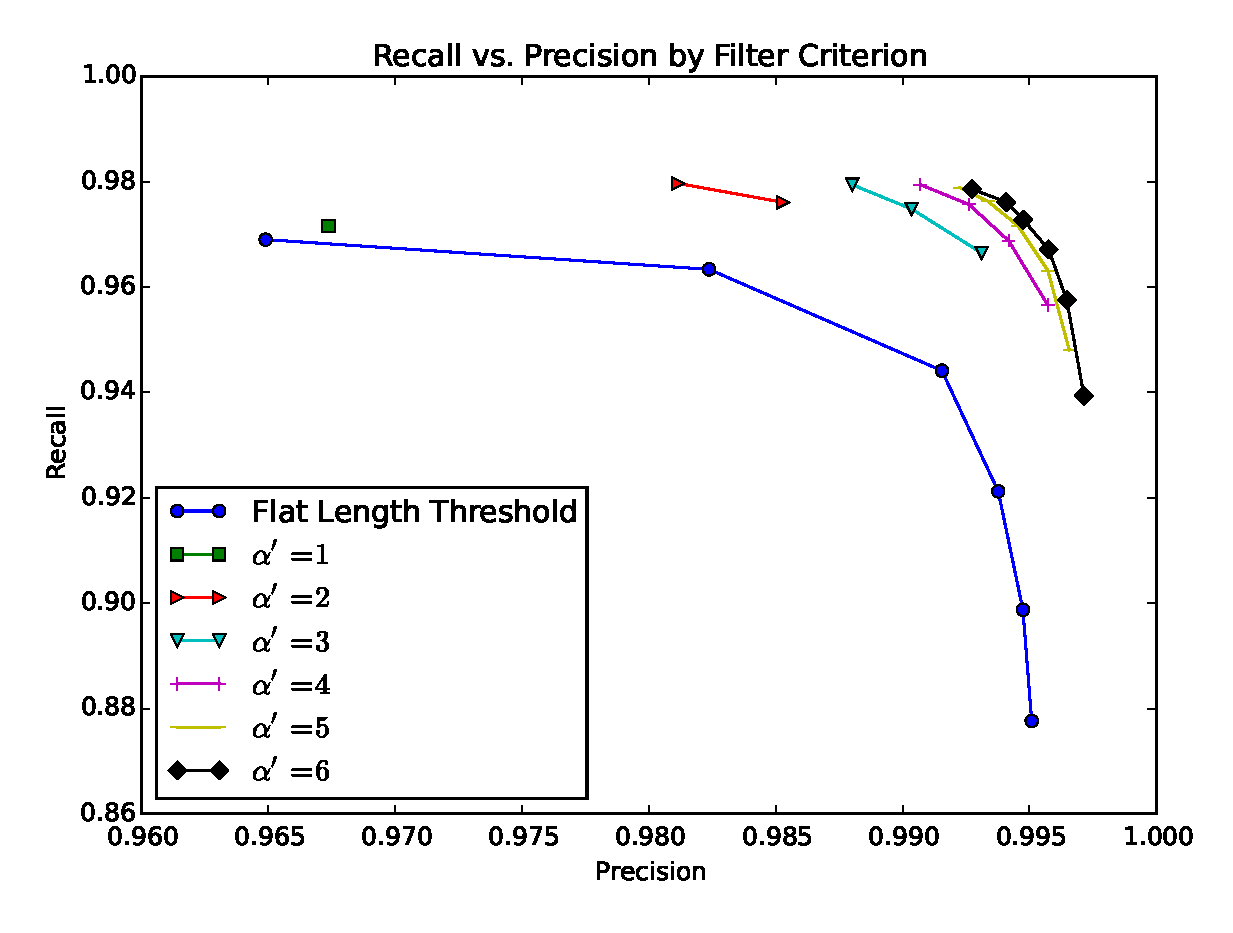
\includegraphics[width=0.5\textwidth]{figures/02_contextschemes/mhcPrecisionRecall.eps}
  }
  \subfloat[]{
  	\label{fig:mhccoverage}
    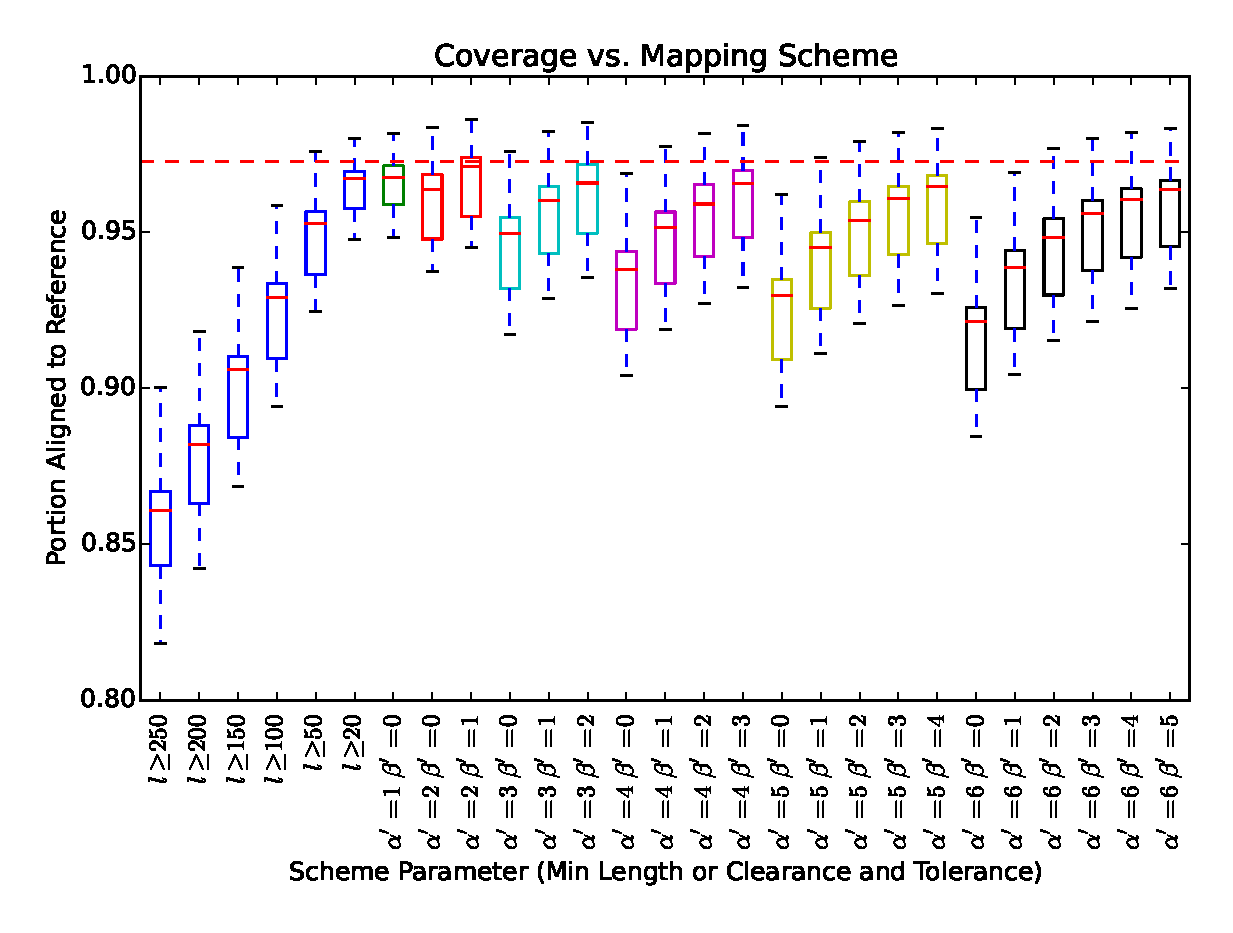
\includegraphics[width=0.5\textwidth]{figures/02_contextschemes/mhcCoverageBar.eps}
  }
  \caption{Results of MHC alignment. Points shown in \ref{fig:mhcprecisionrecall} are averages of alt-loci alignments. Lines connect different $\beta^\prime$ levels for a given $\alpha^\prime$. The red dashed line in \ref{fig:mhccoverage} is the average coverage of the GRC reference alignments.}
  \label{fig:mhc}
\end{figure*}


Mapping schemes using a wide range of $\alpha^\prime$ and $\beta^\prime$ parameters were tried, with $\beta'$ being restricted to values less than $\alpha'$. Additionally, the natural mapping scheme ($\alpha' = 0, \beta' = 0$) was tested, with a parameter used to vary the minimum length of admissible unique substrings (i.e. defining a series of natural context scheme, each only considering unique reference substrings longer than a minimum threshold). 

The strongest performing schemes, in terms of the harmonic mean of precision and recall (F-score), had a precision greater than 0.99 and a recall of around 0.98. Coverage was also remarkably close to that of the GRC reference alignments, suggesting that the conservative nature of the schemes did not result in undue underalignment (Figure~\ref{fig:mhccoverage}). 

In all cases the natural length-thresholded context schemes performed substantially worse than the various $\alpha^\prime$/$\beta^\prime$ combinations in terms of recall of the GRC alignments at a given level of precision (Figure~\ref{fig:mhcprecisionrecall}), and in terms of coverage (Figure~\ref{fig:mhccoverage}). This suggests that $\alpha^\prime$ and $\beta^\prime$ as defined here are effective heuristics. 

Increasing $\alpha'$ for a given $\beta'$ was found to increase precision and decrease recall, but increasing $\beta'$ at a given $\alpha'$ could restore the lost recall (at the cost of precision). The $\alpha' = 5, \beta' = 4$ natural scheme was determined to strike the best balance between precision and recall, as there was a negligible increase in precision between it and the $\alpha' = 6, \beta' = 5$ scheme (Figure~\ref{fig:mhcprecisionrecall}). Both it and the $\alpha' = 3, \beta' = 2$ scheme---selected to provide a good balance between precision and recall while also optimizing for mapping shorter sequences---were chosen for the short sequence mapping tests in \ref{subsec:reads} below.

Two additional configuration options were available for the schemes under test: whether to map unmapped internal bases on credit, and whether to enforce stability over weak stability. Our tests, the results of which are visible in Supplementary Figure~S1a and Supplementary Figure~S4b, demonstrate that requiring stability had a negligible impact on recall for long sequences, while the use of credit produced a sizable gain in recall at a manageable cost in precision (note the scales of the axes in Supplementary Figure~S4b). Consequently, credit was used for all analyses, and the stability requirement was used for the MHC mapping analysis.

\begin{figure}[t]
	\centering
    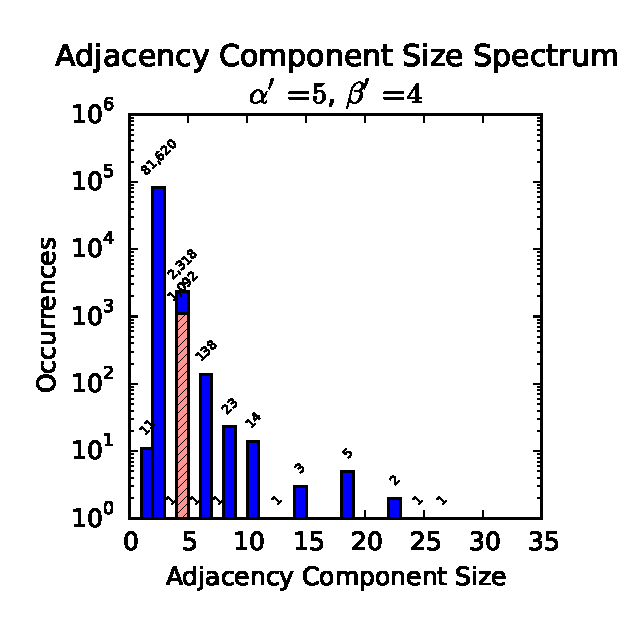
\includegraphics[width=0.3\textwidth]{figures/02_contextschemes/mhcRearrangements.eps}
  \caption{Frequency of rearrangements of different levels of complexity implied by the alignment of MHC alt loci to the primary path, under the $\alpha^\prime = 5$, $\beta^\prime = 4$ natural scheme, which was selected to give the best balance between precision and recall. The X axis shows the number of nodes involved in the rearrangement, while the Y axis shows the number of rearrangements of that size. The red bar shows the number of 4-node rearrangements that are automatically identifiable as tandem duplications.}
  \label{fig:rearrangements}
\end{figure}

%Revised to more precisely define the graph

The $\alpha^\prime = 5$, $\beta^\prime = 4$ natural scheme, which provided the best trade-off between precision and recall, was also evaluated in terms of the number and complexity of rearrangements it invoked to relate the MHC alt loci back to the primary path. Figure~\ref{fig:rearrangements} depicts a ``spectrum'' plot of rearrangement frequency versus size, where a rearrangement is defined as a connected component in a multi-breakpoint/adjacency %Cite needed - Medvedev multi-breakpoint graph/cactus graph theory paper
% BENEDICT TODO: Is this the one you meant?
graph representing the alignment between the primary reference sequence and an alt-loci sequence \citep{medvedev2007computability,paten2011cactus}. Briefly, the nodes of the graph are the ends (sides) of aligned sets of two or more bases and the edges the adjacencies, possibly containing interstitial unaligned sequence, that connect these ends \citep{medvedev2007computability,paten2011cactus}. The spectrum plot shows that the vast majority of rearrangements involve only two nodes (which is the structure of SNPs and simple indels), and of the rearrangements involving 4 nodes, slightly under half of them are recognizable as simple tandem duplications. The tandem duplications, which frequently involve just a handful of bases, are discoverable because of the non-linear nature of context-driven mapping. The remaining, more complex rearrangements have not been identified or named. Supplementary Figure~S5 shows UCSC Genome Browser renderings of some of the rearrangements described in the spectrum plot. 
% TODO: is there a reference to cite for this idea of pinch graphs? See above - Medvedev + cactus paper in JCB.
% See citations above. Would we maybe cite the pinchesAndCacti library?

\subsection{Mapping Simulated Short Reads}
\label{subsec:reads}

Perhaps the most important current application of traditional alignment methods is mapping reads from short read sequencing. To test this scenario a second mapping task was created. Each of the MHC alt loci sequences was broken into overlapping 200bp fragments at 100bp intervals. The read length was chosen to align with that of current or expected near future sequencing technologies, and is near the low end of what the mapping schemes presented here can accommodate \citep{quail2012tale}. Each of these fragments had substitution errors introduced with an independent probability of $1\%$ per base (comparable to current sequencing technologies) \citep{quail2012tale}. We used this simulated scenario, rather than actual reads, because it allowed us to assess the reads' origins to easily determine if mappings were correct or aberrant.


Two variants of the $\alpha'$-$\beta'$-natural scheme ($\alpha' = 3, \beta' = 2$, and $\alpha' = 5, \beta' = 4$), in both stable and weakly stable versions, were used to map each read to the primary path MHC from GRCh38. The results of the popular aligners BWA (using default parameters) and LASTZ (using an empirically-determined restrictive score cut-off), were also included \citep{li2010fast,harris2007improved}. BWA in particular functioned as a gold standard: we did not expect to outperform BWA, but rather sought to recapitulate some of its results in a context-driven framework.

Mapping accuracy was assessed in two ways. First, the number of reads that each mapper could place anywhere in the reference, and portion of bases mapped regardless of correctness, were measured. These results are visible in Figures~\ref{fig:readmappability} and~\ref{fig:readcoverage}, respectively. Second, the number of genes and portion of gene bases with incorrect mappings to other genes, as annotated by the UCSC Genome Browser's ``Known Genes'' database, were also measured, and are visible in Figures~\ref{fig:readgenes} and~\ref{fig:readwrongness} \citep{meyer2013ucsc}.  

%Paralogs
%Reads 
%-- error corrected reads
%-- non-error corrected reads

\begin{figure}[t]
  \centering
  \subfloat[]{
  	\label{fig:readmappability}
    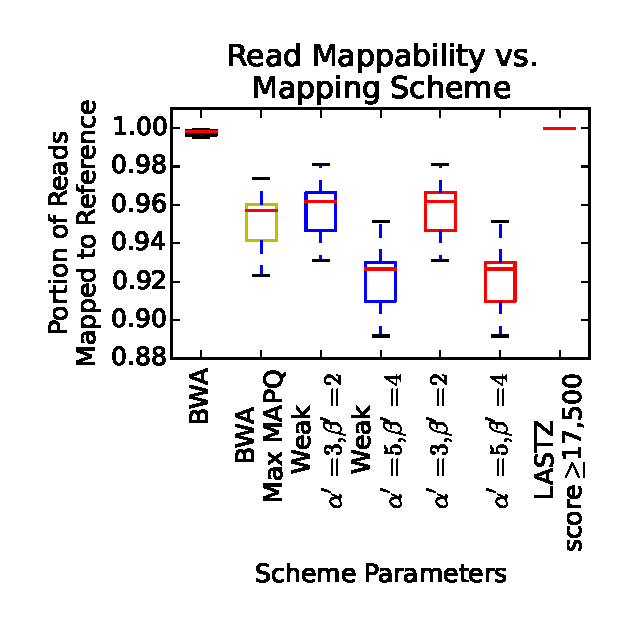
\includegraphics[width=0.5\columnwidth]{figures/02_contextschemes/readMappability.eps}
  }
  \subfloat[]{
  	\label{fig:readcoverage}
    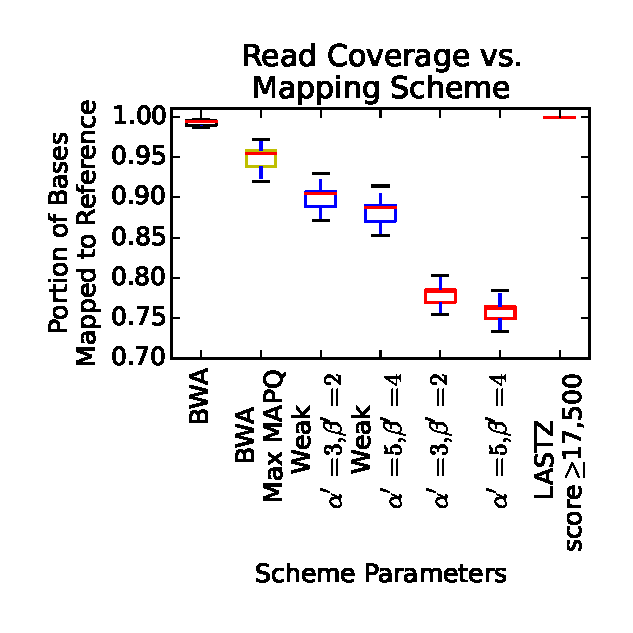
\includegraphics[width=0.5\columnwidth]{figures/02_contextschemes/readCoverage.eps}
  }
  \\
  \subfloat[]{
  	\label{fig:readgenes}
    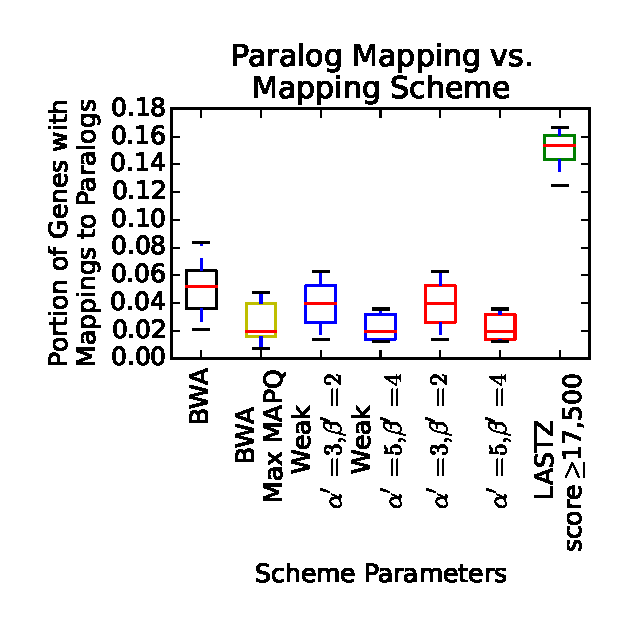
\includegraphics[width=0.5\columnwidth]{figures/02_contextschemes/readGenes.eps}
  }
  \subfloat[]{
  	\label{fig:readwrongness}
    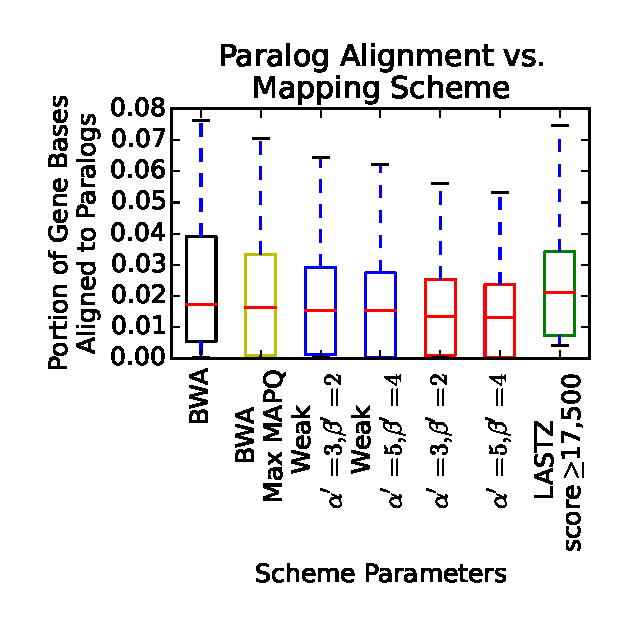
\includegraphics[width=0.5\columnwidth]{figures/02_contextschemes/readWrongness.eps}
  }
  \caption{Results of read alignments. Reads were generated from MHC alt loci by taking tiling 200bp windows at 100bp intervals, and randomly introducing substitution errors at a frequency of $1\%$. Reads were aligned to the GRCh38 primary path MHC region.}
  \label{fig:read}
\end{figure}

%It would be good to look at BWA positions that uniquely map (with no secondary alignments). 
BWA and LASTZ both mapped more of the reads and covered more of the read bases than the context-driven mapping schemes, though the difference was relatively small: less than 10\% in terms of mapped reads and, for the weakly stable context schemes, less than 15\% in terms of coverage. These results were unsurprising, given that a context-driven mapping scheme is a function that can not multi-map any position, while the other two aligners freely produced multi-mappings.

The context-driven mapping schemes examined broadly matched BWA's performance in terms of avoiding mapping genes to their paralogs (Figures~\ref{fig:readgenes} and \ref{fig:readwrongness}). All four context-driven schemes tested outperformed BWA's raw output. However, if BWA's output was filtered to only include reads mapped with maximum mapping quality (which was observed to be 60), only the $\alpha'=5$, $\beta'=4$ natural schemes managed to outperform it in terms of the portion of genes with any mappings to paralogs---and that at a very substantial drop in coverage (Figure~\ref{fig:readcoverage}). LASTZ, on the other hand, did not report mapping qualities; even with what was intended to be a stringent score threshold applied, it produced the most mappings to paralogs of any aligner tested (Figures~\ref{fig:readgenes} and \ref{fig:readwrongness}). 

While the difference between stable and weakly stable mapping schemes was insignificant for long-read mapping, the coverage difference for these shorter reads was much greater. Thus stability, rather than weak stability, might seem an impractical restriction for short reads, albeit one that still admits the mapping of the majority of query sequence elements.

A final experiment characterized the minimum context lengths with which it was possible for a base to map in the GRCh38 primary path MHC; the results are shown in Figure \ref{fig:contexts}. The vast majority of bases were found to be mappable with contexts of 100bp or less, and all but about $2\%$ of bases at $\alpha' = 5$ were found to be mappable with contexts of 200bp or less.


\begin{figure}[t]
  \centering
  \subfloat[]{
  	\label{fig:context}
    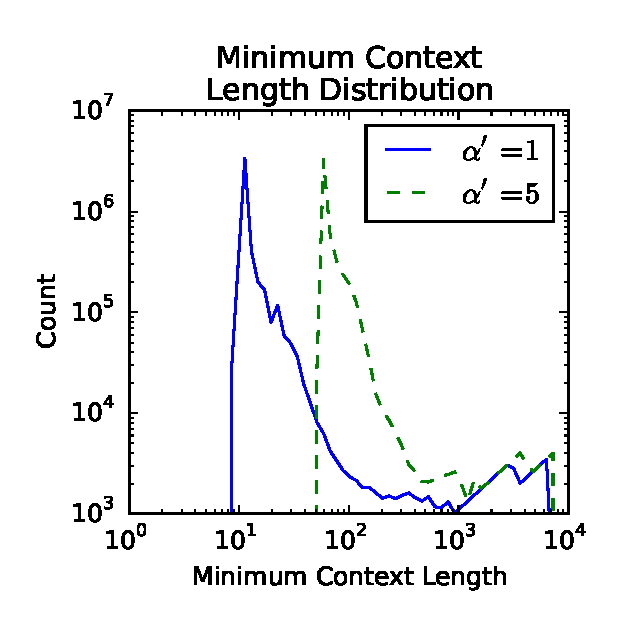
\includegraphics[width=0.5\columnwidth]{figures/02_contextschemes/context.eps}
  }
  \subfloat[]{
  	\label{fig:contextcumulative}
    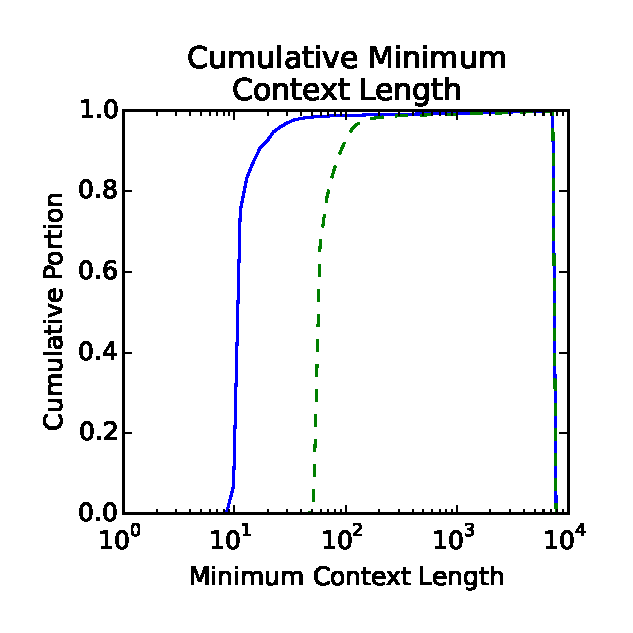
\includegraphics[width=0.5\columnwidth]{figures/02_contextschemes/contextcumulative.eps}
  }
  \caption{Minimum $\beta^\prime = 0$ context lengths required to map uniquely in a reference derived from the GRCh38 primary path MHC, for different $\alpha^\prime$ values. At an $\alpha^\prime$ of $1$, $1.16\%$ of minimal contexts are longer than 100bp, and $0.97\%$ are longer than 200bp. At an $\alpha^\prime$ of $5$, $8.85\%$ of minimal contexts are longer than 100bp, and $1.74\%$ are longer than 200bp}
  \label{fig:contexts}
\end{figure}

\section{Discussion}

%Give overview of benefits (basically the title of the paper)

The new mapping scheme proposed here---both radically different and more conservative than existing methods---has some important benefits. The first is that it is versatile: it can be used to map multi-megabase MHC sequences while accounting for complex rearrangements, but also does reasonably well with 200bp simulated reads. The second major benefit is stability: although requiring stability reduces coverage when mapping short reads, it reveals a majority subset of mapped positions that are aligned globally with high certainty. This is a useful per-base quality assessment somewhat orthogonal and complementary to the widely used read-level mapping quality scores \citep{li2008mapping}.
The third major benefit---being able to define variants in terms of canonical contexts which can diagnose their presence---is related to the second: having a stable mapping scheme enables the articulation of sequences which, when observed, always indicate the presence of a particular variant. This could ultimately pave the way for a high-specificity reference-free method of variant calling, building on the dbSNP concept of flanking strings \citep{sherry2001dbsnp}.

%Discuss how approach is conservative, but that is appropriate for certain cases


% Short sequence mapping

Our results show that the context-driven, stable mapping approach can be more conservative than existing mappers like BWA and LASTZ, at the cost of coverage. If there is any possibility of later having to admit that it was wrong in mapping a base, a stable scheme will not map that base. A weakly stable scheme is only slightly more permissive, willing to map bases only if it knows they cannot possibly map elsewhere. We show that the $\alpha'$-$\beta'$-natural schemes can be much more selective than LASTZ, and can in certain circumstances outperform BWA in avoiding mappings to paralogs, and in the general case are no worse. This specificity comes at the cost of a reduced ability to contend with high sequencing error rates. However, it is particularly important when analyzing regions like the MHC, where some genes present in a query may not be present themselves in the reference to which reads are being mapped, but may nonetheless have close and misleading paralogs in the reference. 
%Indeed, from this small study it is unclear how best to set $\beta'$ to ensure that paralogous mapping is minimized, and

%Cut for brevity
%As would be expected, the weakly stable mapping schemes appear to outperform the stable ones in terms of coverage, in Figure~\ref{fig:readmappability} and Figure~\ref{fig:readcoverage}. The short length of the sequences involved means that many poor MUMs which did not join a sufficiently good $\beta'$-synteny block are nonetheless heuristically regarded as potentially able to do so were the query sequence to be extended. If stability is required, bases which those MUMs cover are ``blacklisted'' and cannot be mapped anywhere. In order to reduce this performance gap, it will be necessary to compute a tighter bound on exactly which MUMs could potentially join a $\beta'$-synteny block with new MUMs that might be created when the query sequence is extended.

% Long sequence mapping
% Detected rearrangements

The $\alpha'$-$\beta'$-natural scheme presented here is more useful for mapping longer sequences, where the costs of stability (incurred only near the sequence ends) are lower, and the chances of finding longer and more distinctive contexts are higher. Longer reads are also more likely to directly exhibit some of the linearity-breaking structural rearrangements that our scheme is designed to deal with. The scheme presented here largely recapitulates the GRC's official alignments. The $\alpha' = 5, \beta' = 4$ instantiation, for example, has approximately $99\%$ precision and $98\%$ recall when compared to the GRC alignments, as depicted in Figure~\ref{fig:mhcprecisionrecall}. Given that the GRC alignments for the MHC alt loci do not contain any duplications, translocations, or inversions, some of the missing precision is almost certainly due to the correct detection of events that the GRC alignments did not completely describe. Judging by our manual analysis (illustrated in Supplementary Figure~S5), such calls are generally plausible. 

%Discuss extension to graphs.
Finally, the context-based mapping scheme method is abstracted from its reference and query inputs, and thus easy to generalize. In addition to being very general in the types of queries it can accept, from short reads to entire alt loci, it is also very general in the types of references it can map to. As long as context sets can be defined for each position, this method can be extended to map to nonlinear, graph-based reference structures (as in Supplementary Figure~S6). Such graph structures, containing common variation in addition to the primary reference, would help to alleviate the reference allele bias inherent in current approaches to variant detection. The mapping scheme presented here provides a concrete approach to mapping to such a structure, something we explored in our earlier paper \citep{paten2014mapping} and that we are actively pursuing. 

Future work to be done on this project includes the creation of a full alignment tool based on the algorithms described here, and an extension of those algorithms to graph-structured references. The software test framework created for this work is available from \url{https://registry.hub.docker.com/u/adamnovak/sequence-graphs/}.

\section*{Acknowledgements}

\paragraph{Funding}
This work was supported by a grant from the Simons Foundation (SFLIFE \#351901). AN was supported by research gift from Agilent Technologies, a fellowship from Edward Schulak, and an award from the ARCS Foundation. Research reported in this publication was also supported by the National Human Genome Research Institute of the National Institutes of Health under Award Number U54HG007990. The content is solely the responsibility of the authors and does not necessarily represent the official views of the National Institutes of Health.



% Chapter 3 is the gPBWT paper, with revisions
\chapter{A Graph Extension of the Positional Burrows-Wheeler Transform and its Applications}
\label{ch:gpbwt}

This chapter has been adapted from the article \citet{novak2016graph}, and contains material attributable to all authors of that work.

\section{Abstract}
WWe present a generalization of the Positional Burrows-Wheeler Transform, or PBWT, to genome graphs, which we call the gPBWT. A genome graph is a collapsed representation of a set of genomes described as a graph. In a genome graph, a haplotype corresponds to a restricted form of walk. The gPBWT is a compressible representation of a set of these graph-encoded haplotypes that allows for efficient subhaplotype match queries. We give efficient algorithms for gPBWT construction and query operations.
As a demonstration, we use the gPBWT to quickly count the number of haplotypes consistent with random walks in a genome graph, and with the paths taken by mapped reads; results suggest that haplotype consistency information can be practically incorporated into graph-based read mappers. We estimate that with the gPBWT of the order of 100,000 diploid genomes, including all forms structural variation, could be stored and made searchable for haplotype queries using a single large compute node.

\section{Introduction}

The PBWT is a compressible data structure for storing haplotypes that provides an efficient search operation for subhaplotype matches \cite{durbin2014efficient}. The PBWT is itself an extension of the ordinary Burrows-Wheeler Transform (BWT), a method for compressing string data \cite{burrows1994block}, with some concepts borrowed from the FM-index, an extension of the BWT that makes it searchable \cite{ferragina2000opportunistic}. Implementations of the PBWT, such as BGT \cite{li2015bgt}, can be used to compactly store and query the haplotypes of thousands of samples. The PBWT can also allow existing haplotype-based algorithms to work on much larger collections of haplotypes than would otherwise be practical \cite{lunter2016fast}. The Haplotype Reference Consortium dataset, for example, contains 64,976 haplotypes \cite{mccarthy2016reference}, and PBWT-based software allows data at this scale to efficiently inform phasing calls on newly sequenced samples, with significant speedups over other methods \cite{loh2016reference}.

In the PBWT each site (corresponding to a genetic variant) is a binary feature and the sites are totally ordered. The input haplotypes to the PBWT are binary strings, with each element in the string indicating the state of a site. In the generalization we present, each input haplotype is a walk in a general bidirected graph, or genome graph. Graph-based approaches to genomics problems like mapping and variant calling have been shown to produce better results than linear-reference-based methods \cite{dilthey2015improved,novak2017genome}, so adapting the PBWT to a graph context is expected to be useful. Other generalizations of BWT-based technologies to the graph context have been published \cite{siren2017indexing,maciuca2016natural,huang2013short}, but they deal primarily with the substring search problem, rather than the problem of storing and querying haplotypes.

The PBWT generalization presented here allows haplotypes to be partial (they can start and end at arbitrary nodes) and to traverse arbitrary structural variation. It does not require the sites (nodes in the graph) to have a biologically relevant ordering to provide compression.
% There still has to be *some* ordering of sides for the sorting of visits to work.
However, despite these generalizations, essential features of the PBWT are preserved. The core data structures are similar, the compression still exploits genetic linkage, and the haplotype matching algorithm is essentially the same. It is expected that this generalization of the PBWT will allow large embedded haplotype panels to inform read-to-graph alignment, graph-based variant calling, and graph-based genomic data visualization, bringing the benefits of the PBWT to the world of genome graphs.

\section{Definitions}

We define $G = (V, E)$ as a \vocab{genome graph} in a bidirected formulation \cite{medvedev2009maximum, paten2014mapping}. Each node in $V$ has a DNA-sequence label; a left, or $5'$, \vocab{side}; and a right, or $3'$, side. Each edge in $E$ is a pairset of sides. The graph is not a multigraph: only one edge may connect a given pair of sides and thus only one \vocab{self-loop}, or edge from a side to itself, can be present on any given side.

While more powerful algorithms are generally used in practice, a simple genome graph can be constructed relatively easily from a reference sequence and a set of nonoverlapping variants (defined as replacements of a nonempty substring of the reference with a nonempty alternate string). Start with a single node containing the entire reference sequence. For each variant to be added, break the nodes in the graph so that the reference allele of the variant is represented by a single node. Then create a node to represent the alternate allele, and attach the left and right sides of the alternate allele to everything that is attached to the left and right, respectively, of the reference allele.

We consider all the sides in the graph to be (arbitrarily) ordered relative to one another. We define the \vocab{null side}, $0$, as a value which corresponds to no actual side in the graph, but which compares less than any actual side. We also define the idea of the \vocab{opposite} of a side $s$, with the notation $\overline{s}$, meaning the side of $s$'s node which is not $s$ (i.e.\ the left side of the node if $s$ is the right side, and the right side of the node if $s$ is the left side). Finally, we use the notation $n(s)$ to denote the node to which a side $s$ belongs.

\hyphenation{ambi-sequence}
To better connect the world of bidirected graphs, in which no orientation is better than any other, and the world of algebra, in which integer subscripts are incredibly convenient, we introduce the concept of an \vocab{ambisequence}. An ambisequence is like a sequence, but the orientation in which the sequence is presented is insignificant; a sequence and its reverse are both equal and opposite \vocab{orientations} of the same underlying ambisequence. An ambisequence is isomorphic to a stick-shaped undirected graph, and the orientations can be thought of as traversals of that graph from one end to the other. For every ambisequence $s$, a canonical orientation is chosen arbitrarily, and the subscripted items $s_{i}$ are the items in that arbitrarily selected sequence. This orientation is also used for defining concepts like ``previous'' and ``next'' in the context of an ambisequence.

Within the graph $G$, we define the concept of a \vocab{thread}, which can be used to represent a haplotype or haplotype fragment. A thread $t$ on $G$ is a nonempty ambisequence of sides, such that for $0 \leq i < N$ sides $t_{2i}$ and $t_{2i+1}$ are opposites of each other, and such that $G$ contains an edge connecting every pair of sides $t_{2i}$ and $t_{2i+1}$. In other words, a thread is the ambisequence version of a walk through the sides of the graph that alternates traversing nodes and traversing edges and which starts and ends with nodes. Note that, since a thread is an ambisequence, it is impossible to reverse. Instead, the ``reverse'' of a thread is one of its two orientations.

We consider $G$ to have associated with it a collection of \vocab{embedded} threads, denoted as $T$. We propose an efficient storage and query mechanism for $T$ given $G$.

\section*{The Graph Positional Burrows-Wheeler Transform}

% This is where we explain why we are going to do what we are about to do.
Our high-level strategy is to store $T$ by grouping together threads that have recently visited the same sequences of sides, and storing in one place the next sides that those threads will visit. As with the Positional Burrows-Wheeler Transform, used to store haplotypes against a linear reference, and the ordinary Burrows-Wheeler Transform, we consider the recent history of a thread to be a strong predictor of where the thread is likely to go next \cite{durbin2014efficient}. By grouping together the next side data such that nearby entries are likely to share values, we can use efficient encodings (such as run-length encodings) and achieve high compression.

More concretely, our approach is as follows. Within an orientation, we call an instance of side in an even-numbered position ${2i}$ a \vocab{visit}; a thread may visit a given side multiple times, in one or both of its orientations. (We define it this way because, while a thread contains both the left and right sides of each node it touches, we only want one visit to stand for the both of them.) Consider all visits of orientations of threads in $T$ to a side $s$. For each visit, take the sequence of sides coming before this arrival at $s$ in the thread and reverse it, and then sort the visits lexicographically by these (possibly empty) sequences of sides, breaking ties by an arbitrary global ordering of the threads. Then, for each visit, look two steps ahead in its thread (past $s$ and $\overline{s}$) to the side representing the next visit, and append it (or the null side if there is no next visit) to a list. After repeating for all the sorted visits to $s$, take that list and produce the array $B_s[]$ for side $s$. An example $B[]$ array and its interpretation are shown in Figure~\ref{fig:barray}. (Note that, throughout, arrays are indexed from $0$ and can produce their lengths trivially upon demand.)  

\begin{figure}[h!]
\centering
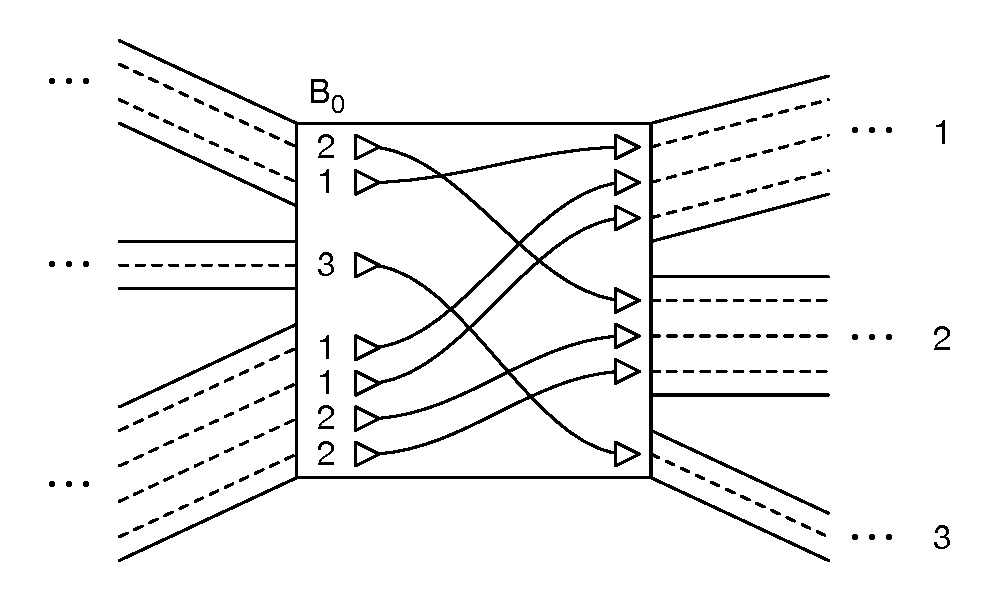
\includegraphics[width=\linewidth]{figures/03_gpbwt/barray.eps}
%Maybe change 0 to s or something.
\caption[An illustration of the {$B_{1}[]$} array]{An illustration of the $B_{1}[]$ array for a single side numbered $1$. (Note that a similar, reverse view could be constructed for the $B_2[]$ array and the opposite orientations of all the thread orientations shown here, but it is omitted for clarity.) The central rectangle represents a node, and the pairs of solid lines on either side delimit edges attached to either the left or right side of the node, respectively. These edges connect the node to other parts of the graph, which have been elided for clarity. The dashed lines within the edges represent thread orientations traveling along each edge in a conserved order, while the solid lines with triangles at the ends within the displayed node represent thread orientations as they cross over one another within the node. The triangles themselves represent ``terminals'', which connect to the corresponding dashed lines within the edges, and which are wired together within the node in a configuration determined by the $B_{1}[]$ array. Thread orientations entering this node by visiting side $1$ may enter their next nodes on sides $3$, $5$, or $7$, and these labels are displayed near the edges leaving the right side of the diagram. (Note that we are following a convention where nodes' left sides are assigned odd numbers, and nodes' right sides are assigned even numbers.) The $B_1[]$ array records, for each thread orientation entering through side $1$, the side on which it enters its next node. This determines through which of the available edges it should leave the current node. Because threads tend to be similar to each other, their orientations are likely to run in ``ribbons'' of multiple thread orientations that both enter and leave together. These ribbons cause the $B_s[]$ arrays to contain runs of identical values, which may be compressed.}
\label{fig:barray}
\end{figure}

Each unoriented edge $\{ s, s' \}$ in $E$ has two orientations $(s, s')$ and $(s', s)$. Let $c()$ be a function of these oriented edges, such that for an oriented edge $( s, s' )$, $c(s, s')$ is the smallest index in $B_{s'}[]$ of a visit of $s'$ that arrives at $s'$ by traversing $\{ s, s' \}$. Note that, because of the global ordering of sides and the sorting rules defined for $B_{s'}[]$ above, $c(s_0, s') \leq c(s_1, s')$ for $s_0 < s_1$ both adjacent to $s'$. Figure~\ref{fig:bstylemultinode} and Table~\ref{tbl:barrays} give a worked example of a collection of $B[]$ arrays and the corresponding $c()$ function values.

%Since sides are globally ordered, oriented edges, as ordered pairs of sides $(s, s')$, can be globally ordered first by $s$ and then by $s'$. For an edge $\{ s, s' \}$ in $G$, $c(s, s')$ gives the number of traversals, within threads in $T$, of oriented edges ending at $s'$ and ordered before $\{s, s'\}$, plus the number of threads beginning at $s$ without first traversing any edges. This is also, due to the definition of $B[]$ above, the smallest index in $B_{s'}[]$ of a visit of $s'$ that arrives at $s'$ by traversing $\{ s, s' \}$, if any such visit exists.

For a given $G$ and $T$, we call the combination of the $c()$ function and the $B[]$ arrays a \vocab{graph Positional Burrows Wheeler Transform (gPBWT)}. We submit that a gPBWT is sufficient to represent $T$, and, moreover, that it allows efficient counting of the number of threads in $T$ that contain a given new thread as a subthread.

\begin{figure}[h!]
\centering
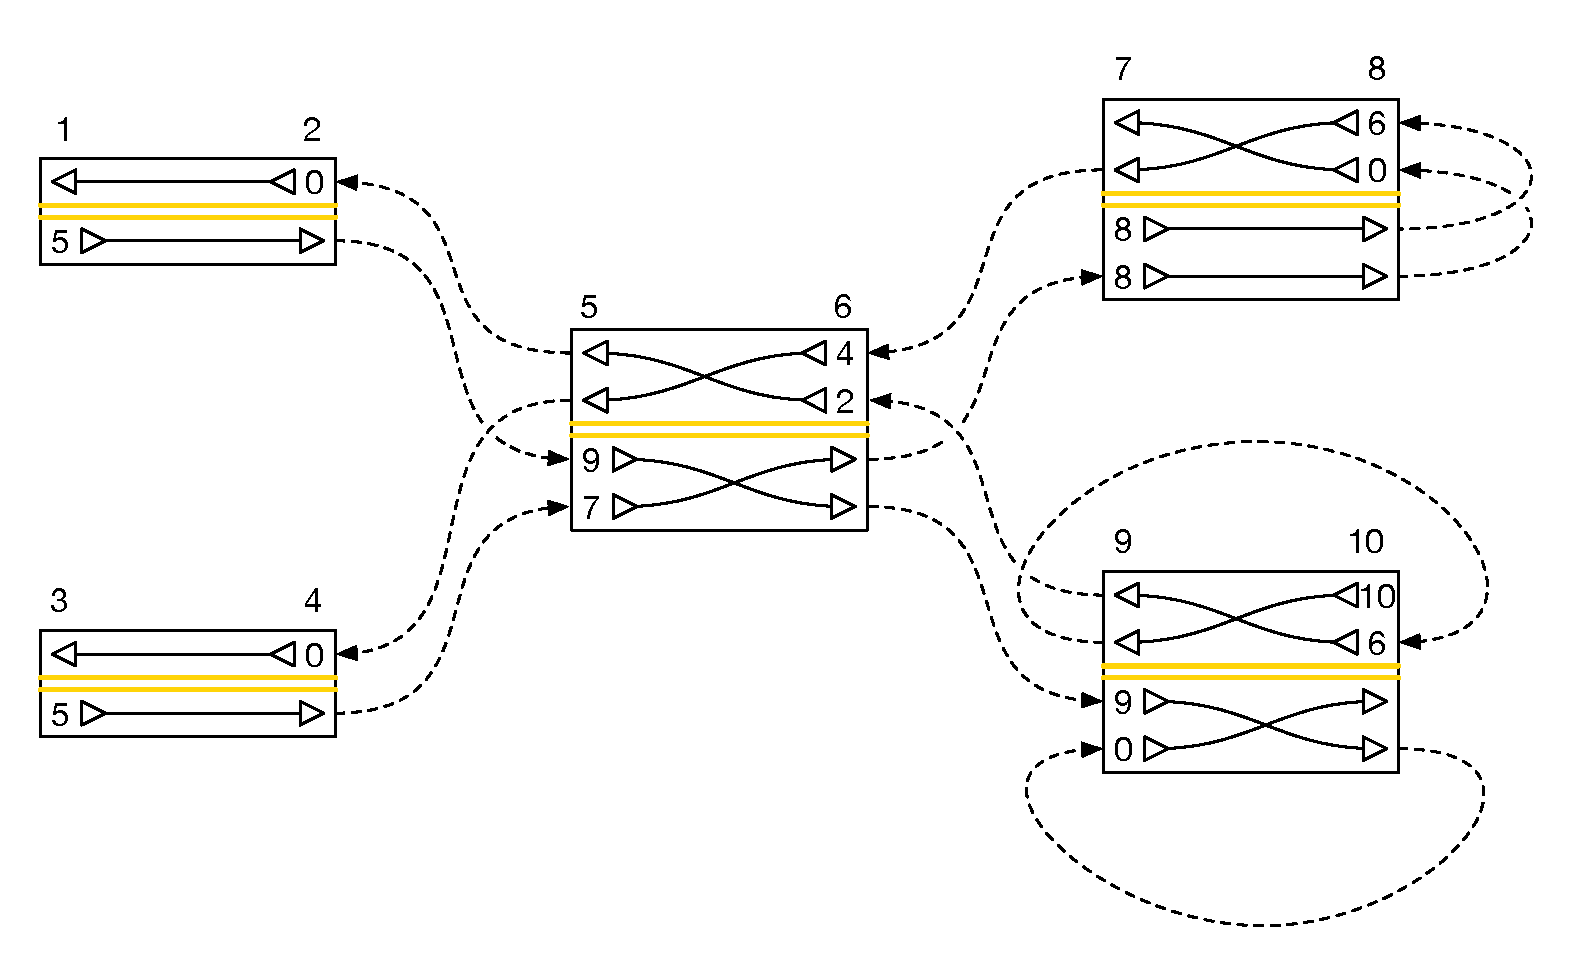
\includegraphics[width=\linewidth]{figures/03_gpbwt/bstylemultinode.eps}
\caption[A diagram of a graph containing two embedded threads]{A diagram of a graph containing two embedded threads. The graph consists of nodes with sides $\{1, 2, 3, \ldots, 10\}$, connected by edges $\{2, 5\}$, $\{4, 5\}$, $\{6, 7\}$, $\{6, 9\}$, $\{8, 8\}$, and $\{10, 9\}$. Note that, once again, odd numbers are used for left sides and even numbers are used for right sides. As in Figure~\ref{fig:barray}, nodes are represented by rectangles, and thread orientations running from node to node are represented by dashed lines. The actual edges connecting the nodes are omitted for clarity; only the thread orientations are shown. Because each side's $B[]$ array defines a separate permutation, each node is divided into two parts by a central double yellow line (like on a road). The top half of each node shows visits to the node's right side, while the bottom half shows visits to the node's left side. Within the appropriate half of each node, the $B[]$ array entries for the entry side are shown. The special $0$ value is used to indicate that a thread stops and does not continue on to another node. When moving from the entry side to the exit side of a node, threads cross over each other so that they become sorted, stably, by the side of their next visit. Threads' order of arrival at a node is determined by the relative order of the edges incident on the side they arrive at, which is in turn determined by the ordering of the sides on the other ends of the edges. The threads shown here are $[1, 2, 5, 6, 9, 10, 9, 10]$ and $[3, 4, 5, 6, 7, 8, 8, 7]$. See Table~\ref{tbl:barrays} for a tabular representation of this example.}
\label{fig:bstylemultinode}
\end{figure}

\begin{table}[h!]
\caption[{$B_s[]$} and {$c()$} values for Figure~\ref{fig:bstylemultinode}]{$B_s[]$ and $c()$ values for the embedding of threads illustrated in Figure~\ref{fig:bstylemultinode}.}
\label{tbl:barrays}
\centering
\begin{tabular} { c | c }
Side & $B_s[]$ Array \\
\hline
$1$ & $[5]$ \\
$2$ & $[0]$ \\
$3$ & $[5]$ \\
$4$ & $[0]$ \\
$5$ & $[9, 7]$ \\
$6$ & $[4, 2]$ \\
$7$ & $[8, 8]$ \\
$8$ & $[6, 0]$ \\
$9$ & $[9, 0]$ \\
$10$ & $[10, 6]$ \\
\end{tabular}
\begin{tabular}{ c | c }
Edge & $c(s, t)$ count \\
\hline
$\{2, 5\}$ & 0 \\
$\{4, 5\}$ & 1 \\
$\{6, 7\}$ & 1 \\
$\{6, 9\}$ & 0 \\
$\{8, 8\}$ & 0 \\
$\{10, 9\}$ & 1 \\
$\{5, 2\}$ & 0 \\
$\{5, 4\}$ & 0 \\
$\{7, 6\}$ & 0 \\
$\{9, 6\}$ & 1 \\
\end{tabular}

\end{table}


\section{Extracting Threads}

To reproduce $T$ from $G$, and the gPBWT, consider each side $s$ in $G$ in turn. Establish how many threads begin (or, equivalently, end) at $s$ by taking the minimum of $c(x, s)$ for all sides $x$ adjacent to $s$. If $s$ has no incident edges, take the length of $B_s[]$ instead. Call this number $b$. Then, for $i$ running from 0 to $b$, exclusive, begin a new thread orientation at $n(s)$ with the sides $[s, \overline{s}]$. Next, we traverse from $n(s)$ to the next node. Consult the $B_s[i]$ entry. If it is the null side, stop traversing, yield the thread orientation, and start again from the original node $s$ with the next $i$ value less than $b$. Otherwise, traverse to side $s' = B_s[i]$. Calculate the arrival index $i'$ as $c(\overline{s}, s')$ plus the number of entries in $B_s[]$ before entry $i$ that are also equal to $s'$ (i.e. the $s'$-\vocab{rank} of $i$ in $B_s[]$). This arrival index, computed by the $\Call{where\_to}{}$ function in Algorithm~\ref{alg:extractThreads}, gives the index in $B_{\overline{s'}}[]$ of the next visit in the thread orientation being extracted.  Then append $s'$ and $\overline{s'}$ to the growing thread orientation, and repeat the traversal process with $i \leftarrow i'$ and $s \leftarrow s'$, until the terminating null side is reached. 

This process will enumerate both orientations of each thread in the graph. The collection of observed orientations can trivially be converted to the collection of underlying ambisequence threads $T$, accounting for the fact that $T$ may contain duplicate threads. Pseudocode for thread extraction is shown in Algorithm~\ref{alg:extractThreads}. The algorithm checks each side for threads, and traces each thread one at a time, doing a constant amount of work at each step (assuming a constant maximum degree for the graph). Therefore, the algorithm runs in $O(M \cdot N + S)$ time for extracting $M$ threads of length $N$ from a graph with $S$ sides. Beyond the space used by the gPBWT itself, the algorithm uses $O(M \cdot N)$ memory, assuming the results are stored.

This algorithm works because the thread orientations embedded in the graph run through it in ``ribbons'' of several thread orientations with identical local history and a conserved relative ordering. The reverse prefix sort specified in the $B[]$ array definition causes thread orientations' visits to a side $s$ that come after the same sequence of immediately prior visits to co-occur in a block in $B_s[]$. For any given next side $s'$, or, equivalently, any edge $(\overline{s}, s')$, the visits to $s'$ that come after visits in that block in $B_s[]$ will again occur together and in the same relative order in a block in $B_{s'}[]$. This is because the visits at side $s'$ will share all the same history that the previous visits shared at side $s$, plus a new previous visit to $s$ that no other visits to $s'$ can share. By finding a visit's index among the visits to $s$ that next take the edge from $\overline{s}$ to $s'$, and by using the $c()$ function to find where in $B_{s'}[]$ the block of visits that just came from $s$ starts, one can find the entry in $B_{s'}[]$ corresponding to the next visit, and thus trace out the whole thread orientation from beginning to end.

\begin{algorithm}[H]
\begin{algorithmic}
\Function{starting\_at}{$Side$, $G$, $B[]$, $c()$}
	\State \Comment{Count instances of threads starting at $Side$.}
    \State \Comment{Replace by an access to a partial sum data structure if appropriate.}
	\If{$Side$ has incident edges}
    	\State \Return $c(s, Side)$ for minimum $s$ over all sides adjacent to $Side$.
    \Else
    	\State \Return $\Call{length}{B_{Side}[]}$
    \EndIf
\EndFunction

\Function{rank}{$b[]$, $Index$, $Item$}
  \State \Comment{Count instances of $Item$ before $Index$ in $b[]$.}
  \State \Comment{Replace by \Call{rank}{} of a rank-select data structure if appropriate.}
  \State $Rank \gets 0$
  \ForAll{index $i$ in $b[]$}
    \If{$b[i] = Item$}
      \State $Rank \gets Rank + 1$
    \EndIf
  \EndFor
  \State \Return $Rank$
\EndFunction

\Function{where\_to}{$Side$, $Index$, $B[]$, $c()$}
\State \Comment{For a thread orientation visiting $Side$ with $Index$ in the reverse prefix sort order, get the corresponding sort index of the next visit in that thread orientation in the side it visits.}
\State \Comment{Works by accounting for all thread orientations starting at the next side or entering the next side via edges before the edge being traversed, and then accounting for the thread orientation's rank among all thread orientations that similarly go from $Side$ to the same next side.}
\State \Return $c(\overline{Side}, B_{Side}[Index]) + \Call{Rank}{B_{Side}[], Index, B_{Side}[Index]}$
\EndFunction

\Function{extract}{$G$, $c()$, $B[]$}
  \State \Comment{Extract all oriented threads from graph $G$.}
  \ForAll{Side $s$ in $G$}
  	\State $TotalStarting \gets \Call{starting\_at}{s, G, B[], c()}$ %h(n(s))$
    \ForAll{$i$ in $[0, TotalStarting)$}
    	\State $Side \gets s$
        \State $Index \gets i$
    	\State $Orientation \gets [s, \overline{s}]$
        \State $NextSide \gets B_{Side}[Index]$
        \While{$NextSide \neq 0$}
          \State $Orientation \gets Orientation + [NextSide, \overline{NextSide}]$
          \State $Index \gets \Call{where\_to}{Side, Index, B[], c()}$
          \State $Side \gets NextSide$
          \State $NextSide \gets B_{Side}[Index]$
        \EndWhile
        \State \Yield $Orientation$
    \EndFor
  \EndFor
\EndFunction
\end{algorithmic}
\caption[Algorithm for extracting threads from a graph]{Algorithm for extracting threads from a graph.}
\label{alg:extractThreads}
\end{algorithm}



\section{Succinct Storage}

For the case of storing haplotype threads specifically, we can assume that, because of linkage, many threads in $T$ are identical local haplotypes for long runs, diverging from each other only at relatively rare crossovers or mutations. Because of the reverse prefix sorting of the visits to each side, successive entries in the $B[]$ arrays are thus quite likely to refer to locally identical haplotypes, and thus to contain the same value for the side to enter the next node on. Thus, the $B[]$ arrays should benefit from run-length compression. Moreover, since (as will be seen below) one of the most common operations on the $B[]$ arrays will be expected to be rank queries, a succinct representation, such as a collection of bit vectors or a wavelet tree \cite{grossi2003high}, would be appropriate. To keep the alphabet of symbols in the $B[]$ arrays small, which is beneficial for such representations, it is possible to replace the stored sides for each $B_s[]$ with numbers referring to the edges traversed to access them, out of the edges incident to $s$.

We note that, for contemporary variant collections (e.g. the 1000~Genomes Project), the underlying graph $G$ may be very large, while there may be relatively few threads (of the order of thousands) \cite{10002015global}. Implementers should thus consider combining multiple $B[]$ arrays into a single data structure to minimize overhead.

\section{Embedding Threads}
% How can we embed an additional thread in a (possibly empty) data structure of this form?

A trivial construction algorithm for the gPBWT is to independently construct $B_s[]$ and $c(s, s')$ for all sides $s$ and oriented edges $(s, s')$ according to their definitions above. However, this would be very inefficient. Here we present an efficient algorithm for gPBWT construction, in which the problem of constructing the gPBWT is reduced to the problem of embedding an additional thread.

Each thread is embedded by embedding its two orientations, one after the other. To embed a thread orientation $t = [t_0, t_1, \ldots t_{2N}, t_{2N+1}]$, we first look at node $n(t_0)$, entering by $t_0$. We insert a new entry for this visit into $B_{t_0}[]$, lengthening the array by one. The location of the new entry is near the beginning, before all the entries for visits arriving by edges, with the exact location determined by the arbitrary order imposed on thread orientations. If no other order of thread orientations suggests itself, the order created by their addition to the graph will suffice, in which case the new entry can be placed at the beginning of $B_{t_0}[]$. The addition of this entry necessitates incrementing $c(s, t_0)$ by one for all oriented edges $(s, t_0)$ incident on $t_0$ from sides $s$ in $G$. We call the location of this entry $k$. The value of the entry will be $t_2$, or, if $t$ is not sufficiently long, the null side, in which case we have finished the orientation. 

If we have not finished the orientation, we first increment $c(s, t_2)$ by one for each side $s$ adjacent to $t_2$ and after $t_1$ in the global ordering of sides. This updates the $c()$ function to account for the insertion into $B_{t_2}[]$ we are about to make.
We then find the index at which the next visit in $t$ ought to have its entry in $B_{t_{2}}[]$, given that the entry of the current visit in $t$ falls at index $k$ in $B_{t_{0}}[]$. This is given by the same procedure used to calculate the arrival index when extracting threads, denoted as $\Call{where\_to}{t_1, k}$ (see Alg.~\ref{alg:extractThreads}). Setting $k$ to this value, we can then repeat the preceding steps to embed $t_2, t_3$, etc. until $t$ is exhausted and its embedding terminated with a null-side entry. Pseudocode for this process is shown in Algorithm~\ref{alg:embeddingThreads}.

As this algorithm proceeds, the $B[]$ arrays are always maintained in the correctly sorted order, because each insertion occurs at the correct location in the array. After each $B[]$ array insertion, the appropriate updates are made to the $c()$ function to keep it in sync with what is actually in the array. Thus, after each thread's insertion, the data structure correctly contains that thread, and so after the insertions of all the relevant threads, a properly constructed gPBWT is produced.

Assuming a dynamic succinct representation, where the $B[]$ array information is both indexed for $O(\log(n))$ rank queries and stored in such a way as to allow $O(\log(n))$ insertion and update (in the length of the array $n$)\footnote{Dynamic data structures at least this good are available as part of the \texttt{DYNAMIC} library, from \url{https://github.com/xxsds/DYNAMIC}.}, this insertion algorithm is $O(N \cdot \log(N + E))$ in the length of the thread to be inserted ($N$) and the total length of existing threads ($E$). Inserting $M$ threads of length $N$ will take $O(M \cdot N \cdot \log(M \cdot N))$ time, and inserting each thread will take $O(N)$ memory in addition to the size of the gPBWT.

\begin{algorithm}[H]
\begin{algorithmic}

\Procedure{insert}{$b[]$, $Index$, $Item$}
  \State \Comment{Insert $Item$ at $Index$ in $b[]$.}
  \State \Comment{Replace by \Call{insert}{} of a rank-select-insert data structure if appropriate.}
  \State $\Call{length}{b[]} \gets \Call{length}{b[]} + 1$ \Comment{Increase length of the array by 1}
  \ForAll{$i$ in $(Index, \Call{length}{b[]} - 1]$, descending}
  	\State $b[i] \gets b[i-1]$
  \EndFor
  \State $b[Index] = Item$
\EndProcedure

\Procedure{increment\_c}{$Side$, $NextSide$, $c()$}
  \State \Comment{Modify $c()$ to reflect the addition of a visit to the edge $(Side, NextSide)$.}
  \ForAll{side $s$ adjacent to $NextSide$ in $G$}
  		\If{$s > Side$ in side ordering}
			\State $c(s, NextSide) \gets c(s, NextSide) + 1$
        \EndIf
  \EndFor
\EndProcedure

\Procedure{embed}{$t$, $G$, $B[]$, $c()$}
  \State \Comment{Embed a thread orientation $t$ in graph $G$.}
  \State \Comment{Call this twice to embed a thread for search in both directions.}
  \State $k \gets 0$ \Comment{Index we are at in $B_{t_{2i}}[]$}
  \State \Call{increment\_c}{$0, t_{0}, c()$} \State \Comment{Increment $c()$ for all edges to $t{0}$, to note a thread start.}
  \ForAll{$i$ in $[0, \Call{length}{t}/2)$}
    \If{$2i + 2 < \Call{length}{t}$}
      \State \Comment{The thread has somewhere to go next.}
      \State \Call{insert}{$B_{t_{2i}}[], k, t_{2i + 2}$} \Comment{Fill in the $B[]$ array slot for this visit.}
      \State \Call{increment\_c}{$t_{2i+1}, t_{2i+2}, c()$} \Comment{Record the traversal of the edge to the next visit.}
      \State $k \gets \Call{where\_to}{t_{2i}, k, B[], c()}$
    \Else
      \State \Call{insert}{$B_{t_{2i}}[], k, 0$} \Comment{End the thread.}
    \EndIf
  \EndFor
\EndProcedure
\end{algorithmic}
\caption[Algorithm for embedding a thread in a graph]{Algorithm for embedding a thread in a graph.}
\label{alg:embeddingThreads}
\end{algorithm}

\section{Batch Embedding Threads}

The embedding algorithm described above, Algorithm~\ref{alg:embeddingThreads}, requires a dynamic implementation for the succinct data structure holding the $B[]$ array information, which can make it quite slow in practice due to the large constant factors involved. In order to produce a more practical implementation, it may be preferable to use a batch construction algorithm, which handles all threads together, instead of one at a time. For the case of directed acyclic graphs (DAGs), such an algorithm is presented here as Algorithm~\ref{alg:dagEmbed}.

This algorithm works essentially like the na\"{\i}ve trivial algorithm of independently constructing every $B_s[]$ for every side $s$ and every $c(s, s')$ for every oriented edge $(s, s')$ from the definitions. However, because of the directed, acyclic structure of the graph, it is able to save redundant work on the sorting steps. Rather than sorting all the threads at each side, it sorts them where they start, and simply combines pre-sorted lists at each side to produce the $B[]$ array ordering, and then stably buckets threads into new sorted lists to pass along to subsequent nodes. The directed, acyclic structure allows us to impose a full ordering on the sides in the graph, so that the sorted lists required by a side all come from ``previous'' sides and are always available when the side is to be processed. 

Although this algorithm requires that all threads be loaded into memory at once in a difficult-to-compress representation (giving it a memory usage of $O(M \cdot N)$ on $M$ threads of length $N$), and although it requires that the graph be a directed acyclic graph, it allows the $B[]$ arrays to be generated for each side in order, with no need to query or insert into any of them. This means that no dynamic succinct data structure is required. Since the graph is acyclic, each thread can visit a side only once, and so the worst case is that a side is visited by every thread. Assuming a constant maximum degree for the graph, since the algorithm visits each side only once, the worst-case running time is $O(M \cdot S)$ for inserting $M$ threads into a graph with $S$ sides.

This algorithm produces the same gPBWT, in the form of the $B[]$ arrays and the $c()$ function, as the single-thread embedding algorithm would.

\begin{algorithm}[H]
\begin{algorithmic}
\Function{batch\_embed\_into\_dag}{$T$, $G$}
	\State \Comment{Construct the gPBWT for threads $T$ embedded in directed acyclic graph $G$.}
    \State \Comment{The forward orientation of each $t$ must flow forwards through the forward orientation of $G$.}
    \State Create empty $B_s[]$ for each side $s$ in $G$
    \State Create empty $c()$
    \ForAll{$o$ in $[\texttt{FORWARD}, \texttt{REVERSE}]$}
    	\State $Messages \gets []$
    	\State $ThreadsByStart \gets []$
        \ForAll{$t$ in $T$}
        	\State $t' \gets t$ in orientation $o$
    		\State $ThreadsByStart[t'_{0}] \gets t'$
            \State \Call{increment\_c}{$0, t'_{0}, c()$} \State \Comment{Increment $c()$ for all edges to $t'_{0}$, to note a thread start.}
    	\EndFor
    	\ForAll{leading side $s$ in $G$ traversed in orientation $o$}
        	\State $ThreadsHere \gets []$
            \ForAll{$t'$ in $ThreadsByStart[s]$}
            	\State $ThreadsHere \gets ThreadsHere + [(t', 0)]$
            \EndFor
            \ForAll{edge $(s', s)$ in $G$, in order}
            	\State \Comment{Collect messages coming along edges to $s$.}
            	\State $ThreadsHere \gets ThreadsHere + Messages[(s', s)]$
                \State $Messages[(s', s)] \gets []$
            \EndFor
            \ForAll{$(t', n)$ at index $i$ in $ThreadsHere$}
            	\State $n \gets n + 1$
            	\If{$\Call{length}{t'} > n * 2$}
                	\State $NextSide \gets t'[n * 2]$
                    \State $Messages[(\overline{s}, NextSide)] \gets Messages[(\overline{s}, NextSide)] + [(t', n)]$
                	\State \Call{increment\_c}{$\overline{s}, NextSide, c()$}
                \Else
                	\State $NextSide \gets 0$
                \EndIf
            	\State $B_s[i] \gets NextSide$
            \EndFor
        \EndFor
    \EndFor
    \State \Return $B[], c()$
\EndFunction
\end{algorithmic}
\caption[Algorithm for embedding all threads at once into a directed acyclic graph]{Algorithm for embedding all threads at once into a directed acyclic graph.}
\label{alg:dagEmbed}
\end{algorithm}

\section{Counting Occurrences of Subthreads}
% Given a new thread, how can we count matching threads? And how can we do it in such a way that extending the query thread is O(1)?

The generalized PBWT data structure presented here preserves some of the original PBWT's efficient haplotype search properties \cite{durbin2014efficient}. The algorithm for counting all occurrences of a new thread orientation $t$ as a subthread of the threads in $T$ runs as follows.

We define $f_i$ and $g_i$ as the first and past-the-last indexes for the range of visits of orientations of threads in $T$ to side $t_{2i}$, ordered as in $B_{t_{2i}}[]$.
% Removing this clause, unnecessary:, such that $t_0 \ldots t_{2i}$ is a suffix of each visit's thread ending at the visit. 

For the first step of the algorithm, $f_0$ and $g_0$ are initialized to $0$ and the length of $B_{t_0}[]$, respectively, so that they select all visits to node $n(t_0)$, seen as entering through $t_0$. On subsequent steps, $f_{i+1}$ and $g_{i+1}$, are calculated from $f_i$ and $g_i$ merely by applying the $\Call{where\_to}{}$ function (see Alg.~\ref{alg:extractThreads}). We calculate $f_{i+1} = \Call{where\_to}{t_{2i}, f_i}$ and $g_{i+1} = \Call{where\_to}{t_{2i}, g_i}$.

This process can be repeated until either $f_{i+1} \geq g_{i+1}$, in which case we can conclude that the threads in the graph have no matches to $t$ in its entirety, or until $t_{2N}$, the last entry in $t$, has its range $f_N$ and $g_N$ calculated, in which case $g_N - f_N$ gives the number of occurrences of $t$ as a subthread in threads in $T$. Moreover, given the final range from counting the occurrences for a thread $t$, we can count the occurrences of any longer thread that begins (in its forward orientation) with $t$, merely by continuing the algorithm with the additional entries in the longer thread.

This algorithm works because the sorting of the $B[]$ array entries by their history groups entries for thread orientations with identical local histories together into contiguous blocks. On the first step, the block for just the orientations visiting the first side is selected, and on subsequent steps, the selected block is narrowed to just the orientations that visit the current side and which share the sequence of sides we have previously used in their history. The $\Call{where\_to}{}$ function essentially traces where the first and last possible consistent thread orientations would be inserted in the next $B[]$ array, and so produces the new bounds at every step.

Assuming that the $B[]$ arrays have been indexed for $O(1)$ rank queries (which is possible using available succinct data structure libraries such as \cite{gog2014theory}, when insert operations are not required), the algorithm is $O(N)$ in the length of the subthread $t$ to be searched for, and has a runtime independent of the number of occurrences of $t$. It can be performed in a constant amount of memory ($O(1)$) in addition to that used for the gPBWT. Pseudocode is shown in Algorithm~\ref{alg:subthreadSearch}.

\begin{algorithm}[H]
\begin{algorithmic}
\Function{count}{$t$, $G$, $B[]$, $c()$}
  \State \Comment{Count occurrences of subthread $t$ in graph $G$.}
  \State $f \gets 0$
  \State $g \gets \Call{length}{B_{t_{0}}[]}$
  \ForAll{$i$ in $[0, \Call{length}{t}/2 - 1)$}
    \State $f \gets \Call{where\_to}{t_{2i}, f, B[], c()}$
    \State $g \gets \Call{where\_to}{t_{2i}, g, B[], c()}$
    \If{$f \geq g$}
    	\State \Return 0
    \EndIf
  \EndFor
  \State \Return $g - f$
\EndFunction
\end{algorithmic}
\caption[Algorithm for searching for a subthread in the graph]{Algorithm for searching for a subthread in the graph.}
\label{alg:subthreadSearch}
\end{algorithm}

% Implementation possibilities:
% https://github.com/nicolaprezza/DYNAMIC
% http://arxiv.org/pdf/1005.4652.pdf
% libmaus2: https://github.com/gt1/libmaus2/blob/master/src/libmaus2/wavelet/DynamicWaveletTree.hpp
% We really do want dynamic rank and select if we're going to build the graph by repeated inserts (or we're going to end up updating lots of partial sums...)

\section{Results}

The gPBWT was implemented within \texttt{xg}, the succinct graph indexing component of the \texttt{vg} variation graph toolkit \cite{garrison2016vg}. The primary succinct self-indexed data structure used, which compressed the gPBWT's $B[]$ arrays, was a run-length-compressed wavelet tree, backed by sparse bit vectors and a Huffman-shaped wavelet tree, all provided by the \texttt{sdsl-lite} library used by \texttt{xg} \cite{gog2014theory}. The $B[]$ arrays, in this implementation, were stored as small integers referring to edges leaving each node, rather than as full next-side IDs. The $c()$ function was implemented using two ordinary integer vectors, one storing the number of threads starting at each side, and one storing the number of threads using each side and each oriented edge. Due to the use of \texttt{sdsl-lite}, and the poor constant-factor performance of dynamic alternatives, efficient integer vector insert operations into the $B[]$ arrays were not possible, and so the batch construction algorithm (Alg.~\ref{alg:dagEmbed}), applicable only to directed acyclic graphs, was implemented. A modified release of \texttt{vg}, which can be used to replicate the results shown here, is available from \url{https://github.com/adamnovak/vg/releases/tag/gpbwt2}.

The modified \texttt{vg} was used to create a genome graph for human chromosome 22, using the 1000~Genomes Phase 3 VCF on the hg19 assembly, embedding information about the correspondence between VCF variants and graph elements \cite{10002015global}. Note that the graph constructed from the VCF was directed and acyclic; it described only substitutions and indels, with no structural variants, and thus was amenable to the batch gPBWT construction algorithm. Next, haplotype information for the 5,008~haplotypes stored in the VCF was imported and stored in a gPBWT-enabled \texttt{xg} index for the graph, using the batch construction algorithm mentioned above. In some cases, the VCF could not be directly translated into self-consistent haplotypes. For example, a \texttt{G} to \texttt{C} SNP and a \texttt{G} to \texttt{GAT} insertion might be called at the same position, and a haplotype might claim to contain the alt alleles of both variants. A na\"{\i}ve interpretation might have the haplotype visit the \texttt{C} and then the \texttt{GAT}, which would be invalid, because the graph would not contain the \texttt{C} to \texttt{G} edge. In cases like this, an attempt was made to semantically reconcile the variants automatically (in this case, as a \texttt{C} followed by an \texttt{AT}), but this was only possible for some cases. In other cases, invalid candidate haplotype threads were still generated. These were then split into valid pieces to be inserted into the gPBWT. Threads were also split to handle other exceptional cases, such as haploid calls in the input. Overall, splitting for causes other than loss of phasing occurred 203,145~times across the 5,008~haplotypes, or about 41~times per haplotype.

The \texttt{xg} indexing and gPBWT construction process took 9~hours and~19 minutes using a single indexing thread on an Intel Xeon X7560 running at 2.27~GHz, and consumed 278~GB of memory. The high memory usage was a result of the decision to retain the entire data set in memory in an uncompressed format during construction. However, the resulting \texttt{xg} index was 436~MB on disk, of which  321~MB was used by the gPBWT. Information on the 5,008~haplotypes across the 1,103,547~variants was thus stored in about 0.93~bits per diploid genotype in the succinct self-indexed representation, or 0.010 bits per haplotype base. \footnote{The improved size results here relative to the results in our conference paper are related to the use of a new run-length-compressed storage backend for the $B[]$ arrays, replacing one that was previously merely succinct \cite{novak2016graph}.} Extrapolating linearly from the 51~megabases of chromosome 22 to the entire 3.2~gigabase human reference genome, a similar index of the entire 1000~Genomes dataset would take 27~GB, with 20~GB devoted to the gPBWT. This is well within the storage and memory capacities of modern computer systems.

\subsection{Random Walks}

The query performance of the gPBWT implementation was evaluated using random walk query paths. 1 million random walks of 100~bp each were simulated from the graph. To remove walks covering ambiguous regions, walks that contained two or more \texttt{N} bases in a row were eliminated, leaving 686,590~random walks. The number of haplotypes in the gPBWT index consistent with each walk was then determined, taking 61.29~seconds in total using a single query thread on the above-mentioned Xeon system. The entire operation took a maximum of 458~MB of memory, indicating that the on-disk index did not require significant expansion during loading to be usable. Overall, the gPBWT index required 89.3~microseconds per count operation on the 100~bp random walks. It was found that 316,078~walks, or 46\%, were not consistent with any haplotype in the graph. The distribution of of the number of haplotypes consistent with each random walk is visible in Figure~\ref{fig:consistenthaplotypes}. 

\subsubsection{Read Alignments}

To further evaluate the performance of the query implementation, we evaluated read alignments to measure their consistency with stored haplotypes. 1000~Genomes Low Coverage Phase 3 reads for NA12878 that were mapped in the official alignment to chromosome 22 were downloaded and re-mapped to the chromosome 22 graph, using the \texttt{xg}/GCSA2-based mapper in \texttt{vg}, allowing for up to a single secondary mapping per read. (The \texttt{vg} aligner was chosen because of its ease of integration with our \texttt{xg}-based gPBWT implementation, but in principle any aligner that supports aligning to a graph could be used.) The mappings with scores of at least 90~points out of a maximum of 101~points (for a perfectly-mapped 101~bp read) were selected (thus filtering out alignments highly like to be erroneous) and broken down into primary and secondary mappings. The number of haplotypes in the gPBWT index consistent with each read's path through the graph was calculated (Fig.~\ref{fig:consistenthaplotypes}). For 1,500,271~primary mappings, the count operation took 150.49~seconds in total, or 100~microseconds per mapping, using 461~MB of memory. (Note that any approach that depended on visiting each haplotype in turn, such as aligning each read to each haplotype, would have to do its work for each read/haplotype combination in less than 20 microseconds, or about 45 clock cycles, in order to beat this time.) It was found that 2,521 of these primary mappings, or 0.17\%, and 320 of 43,791~secondary mappings, or 0.73\%, were not consistent with any haplotype path in the graph. \footnote{These numbers are expected to differ from those reported in our conference paper due to improvements to the \texttt{vg} mapping algorithms since the conference paper was prepared  \cite{novak2016graph}.} These read mappings, despite having reasonable edit based scores, may represent rare recombinations, but the set is also likely to be enriched for spurious mappings.


\begin{figure}[h!]
\centering
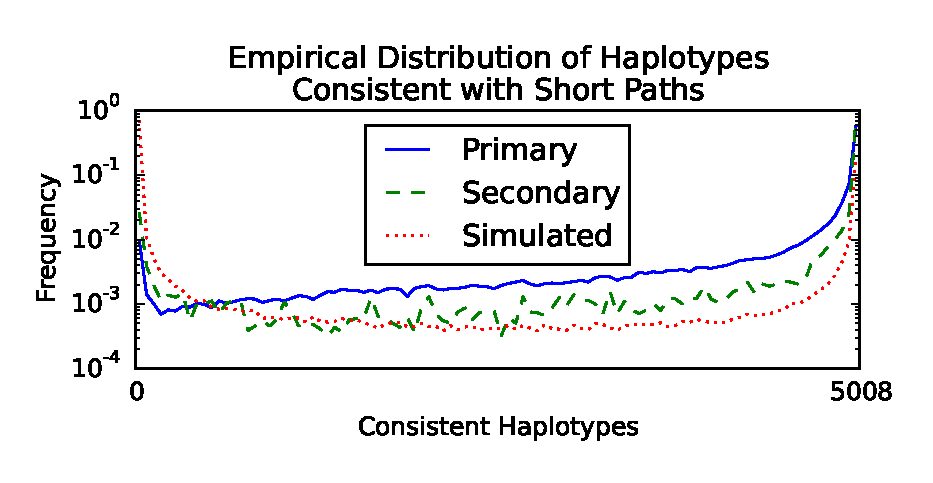
\includegraphics[width=\linewidth]{figures/03_gpbwt/histogram.eps}
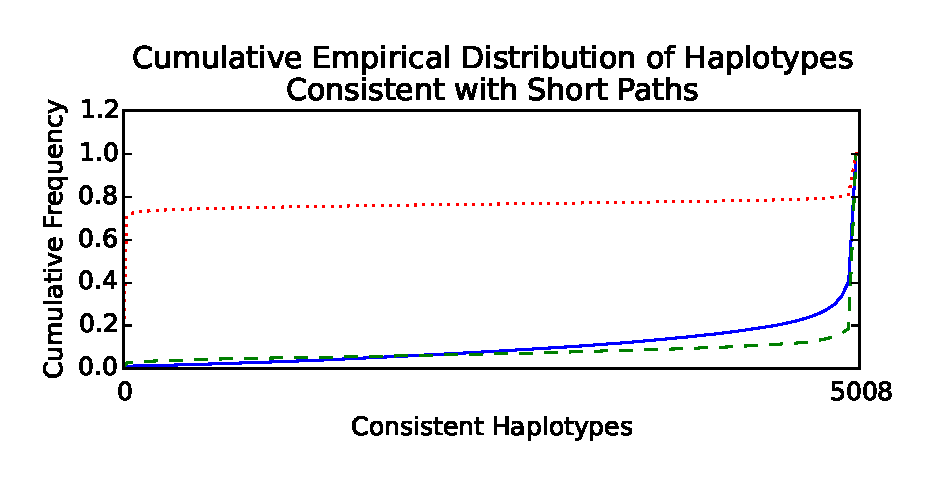
\includegraphics[width=\linewidth]{figures/03_gpbwt/cumulative.eps}
\caption[Consistent haplotypes]{Distribution (top) and cumulative distribution (bottom) of the number of 1000~Genomes Phase 3 haplotypes consistent with short paths in the hg19 chromosome 22 graph. Primary mappings of 101~bp reads with scores of 90 out of 101 or above ($n=1,500,271$) are the solid blue line. Secondary mappings meeting the same score criteria ($n=43,791$) are the dashed green line. Simulated 100~bp random walks in the graph without consecutive \texttt{N} characters ($n=686,590$) are the dotted red line. Consistent haplotypes were counted using the gPBWT support added to \texttt{vg} \cite{garrison2016vg}.}
\label{fig:consistenthaplotypes}
\end{figure}


% Briefly describe implementation in xg and link to code
% Describe storing 1000-G haplotype data and give compression statistics

%Map Q scores with recombination
% TODO: MAPQ won't be done by the time we want to submit this, so I'm going to cut it - Adam

\subsection{Scaling Characteristics}

To evaluate the empirical space usage scaling characteristics of our gPBWT implementation, a scaling experiment was undertaken. The 1000 Genomes VCFs Phase 3 VCFs for the GRCh38 assembly were downloaded, modified to express all variants on the forward strand in the GRCh38 assembly, and used together with the assembly data to produce a graph for chromosome~22 based on the newer assembly. This graph was then used to construct a gPBWT with progressively larger subsets of the available samples. Samples were selected in the order they appear in the VCF file. For each subset, an \texttt{xg} serialization report was generated using the \texttt{xg} tool, and the number of bytes attributed to ``threads'' was recorded. The number of bytes used versus the number of samples stored is displayed in Figure~\ref{fig:scaling}.

\begin{figure}[h!]
\centering
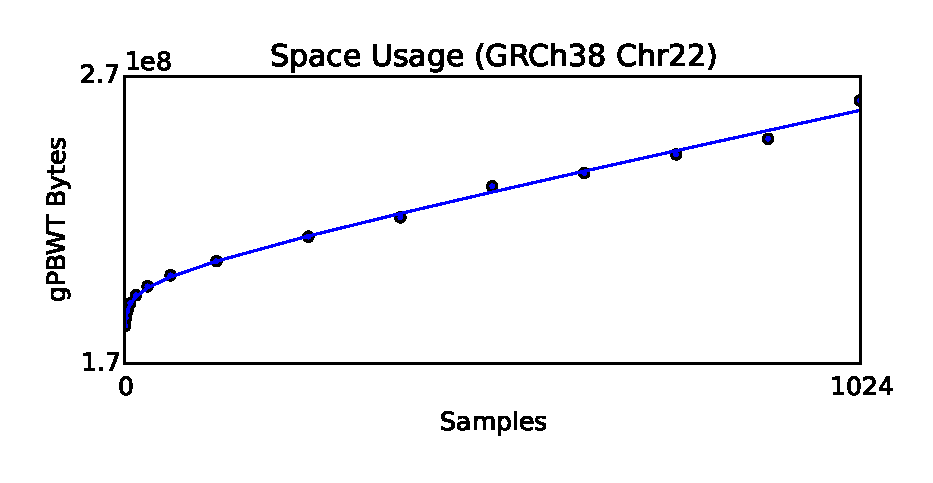
\includegraphics[width=\linewidth]{figures/03_gpbwt/scaling.eps}
\caption[Disk space usage for the gPBWT]{Disk space usage for the gPBWT versus sample count for GRCh38 chromosome~22. Points are sampled at powers of two up to 128, and intervals of 128 thereafter up to 1024. The trend line shown corresponds to the function $y(x) = \num{3.16E6}~\mathrm{bytes} \cdot \ln(x / \mathrm{samples}) + \num{5.12E4}~\frac{\mathrm{bytes}}{\mathrm{sample}} \cdot x + \num{1.84E8}~\mathrm{bytes}$.}
\label{fig:scaling}
\end{figure}

After empirical size data was obtained, a log-plus-linear curve, consisting of a log component and a linear component, was fit to the data. This curve was used to extrapolate an estimated size of 5.34~GB on disk for the storage of 100,000 samples' worth of data on chromosome~22. We choose 100,000 because it is representative of the scale of large contemporary sequencing projects, such as Genomics England's 100,000 Genomes Project (\url{https://www.genomicsengland.co.uk/the-100000-genomes-project/}) \cite{nothaft2015rethinking} and the NHLBI's TOPMed program (\url{https://www.nhlbi.nih.gov/research/resources/nhlbi-precision-medicine-initiative/topmed}). Linear extrapolation from the 51~megabase chromosome~22 to the 3.2~gigabase human genome yields a size estimate of 336~GB for the storage of 100,000 diploid genomes, in addition to the space usage of the underlying graph. Although this extrapolation does not account for the dependence of graph complexity on the number of samples sequenced, it suggests that the gPBWT is capable of scaling to the anticipated size of future sequencing data sets, while using currently available computing resources.

\section{Discussion}

We have introduced the gPBWT, a graph based generalization of the PBWT. We have demonstrated that a gPBWT can be built for a substantial genome graph (all of human chromosome 22 and the associated chromosome 22 substitutions and indels in 1000~Genomes). Using this data structure, we have been able to quickly determine that the haplotype consistency rates of random walks and primary and secondary read mappings differ substantially from each other, and based on the observed distributions we hypothesize that consistency with very few haplotypes can be a symptom of a poor alignment. 

Such poor alignments could arise by a variety of means, including similarity between low complexity sequence, or paralogy; the latter representing true sequence homology but not true sequence orthology. Paralogous alignments are often difficult to distinguish from truly orthologous alignments, and can lead to the reporting of false or misplaced variants. Using haplotype consistency information is one way we might better detect paralogy, because paralogous sequence is not expected to be consistent with linkage relationships at a paralogous site. A more sophisticated analysis of haplotype consistency rate distributions could thus improve alignment scoring.

\begin{sloppypar}
In the present experiment, we have examined only relatively simple variation: substitutions and short indels. Instances of more complex variation, like large inversions and translocations, which would have induced cycles in our genome graphs, were both absent from the 1000 Genomes data set we used and unsupported by the optimized DAG-based construction algorithm which we implemented. We expect that complex structural variation is well suited to representation as a genome graph, so supporting it efficiently should be a priority for a serious practical gPBWT construction implementation.
\end{sloppypar}

\begin{sloppypar}
Extrapolating from our results on chromosome 22, we predict that a whole-genome gPBWT could be constructed for all 5,008 haplotypes of the 1000~Genomes data on GRCh37 and stored in the main memory of a reasonably apportioned computer, using about 27~GB of memory for the final product. On the GRCh38 data set, we extrapolate a space usage of 21~GB for the 2,504 samples of the 1,000~Genomes Project; A whole-genome gPBWT for 100,000~samples on GRCh38, we predict, could be stored in about 336~GB. Computers with this amount of memory, though expensive, are readily available from major cloud providers. (The wasteful all-threads-in-memory construction implementation we present here, however, would not be practical at such a scale, requiring on the order of 50~TB of memory to handle 100,000~samples when constructing chromosome 1; a disk-backed implementation or other low-memory construction algorithm would be required.) The relatively modest growth from 5,008 haplotypes (2,504 samples) to 200,000 haplotypes (100,000 samples) is mostly attributable to the run-length compression used to store the $B$ arrays in our implementation. Each additional sample is representable as a mere increase in run lengths where it agrees with previous samples, and contributes an exponentially diminishing number of new variants and novel linkage patterns. While further empirical experimentation will be necessary to reasonably extrapolate further, it does not escape our notice that the observed scaling patterns imply the practicality of storing cohorts of a million or more individuals, such as those envisaged by the Precision Medicine Initiative \cite{hudson2015precision} and other similar national efforts, within an individual powerful computer. Looking forward, this combination of genome graph and gPBWT could potentially enable efficient mapping not just to one reference genome or collapsed genome graph, but simultaneously to an extremely large set of genomes related by a genome graph.
\end{sloppypar}

\section{List of Abbreviations}
\begin{itemize}
\item \textbf{BWT}: Burrows-Wheeler Transform
\item \textbf{PBWT}: Positional Burrows-Wheeler Transform
\item \textbf{gPBWT}: Graph Positional Burrows-Wheeler Transform
\item \textbf{GRC}: Genome Reference Consortium
\item \textbf{GRCh37}: GRC human genome assembly, build 37
\item \textbf{GRCh37}: GRC human genome assembly, build 38
\item \textbf{DAG}: Directed Acyclic Graph
\end{itemize}

\section{Declarations}

\subsection{Ethics approval and consent to participate}
All human data used in this study comes from already published, fully public sources, namely the 1000 Genomes Project and the human reference assembly. We believe that the work performed in this study is consistent with the purpose for which these data resources were created, and that the original ethical reviews of the creation and publication of these data resources, and the consent assertions given to the original projects, are sufficient to cover this new work.

\subsection{Consent for publication}
Not applicable

\subsection{Availability of data and material}
\begin{sloppypar}
The datasets analyzed during the current study are available in the 1000 Genomes repository, at \url{ftp://ftp.1000genomes.ebi.ac.uk/vol1/ftp/release/20130502/ALL.chr22.phase3_shapeit2_mvncall_integrated_v5a.20130502.genotypes.vcf.gz} (md5 \texttt{ad7d6e0c05edafd7faed7601f7f3eaba}), \url{ftp://ftp.1000genomes.ebi.ac.uk/vol1/ftp/release/20130502/ALL.chr22.phase3_shapeit2_mvncall_integrated_v5a.20130502.genotypes.vcf.gz.tbi} (md5 4202e9a481aa8103b471531a96665047), \url{ftp://ftp.1000genomes.ebi.ac.uk/vol1/ftp/technical/reference/phase2_reference_assembly_sequence/hs37d5.fa.gz} (md5 \texttt{a07c7647c4f2e78977068e9a4a31af15}), and \url{ftp://ftp.1000genomes.ebi.ac.uk/vol1/ftp/release/20130502/supporting/GRCh38_positions/ALL.chr22.phase3_shapeit2_mvncall_integrated_v3plus_nounphased.rsID.genotypes.GRCh38_dbSNP_no_SVs.vcf.gz} (md5 \texttt{cf7254ef5bb6f850e3ae0b48741268b0}), and in the GRCh38 assembly repository, at \url{ftp://ftp.ncbi.nlm.nih.gov/genomes/all/GCA/000/001/405/GCA_000001405.15_GRCh38/GCA_000001405.15_GRCh38_assembly_structure/Primary_Assembly/assembled_chromosomes/FASTA/chr22.fna.gz} (md5 \texttt{915610f5fb9edfcc9ce477726b9e72c6}).
\end{sloppypar}

\section{Competing interests}
The authors declare that they have no competing interests.

\subsection{Funding}
This work was supported by the National Human Genome Research Institute of the National Institutes of Health under Award Number 5U54HG007990, the W.M. Keck foundation under DT06172015, the Simons Foundation under SFLIFE\# 351901, the ARCS Foundation, and Edward Schulak. The content is solely the responsibility of the authors and does not necessarily represent the official views of the National Institutes of Health or any other funder.

\section{Author's contributions}
    A.M.N. wrote most of the gPBWT implementation presented here, conducted the experiments, and composed the majority of the manuscript. E.G. managed the \texttt{vg} project, wrote the read simulation and mapping code used here, and collaborated on the gPBWT implementation. B.P. developed the mathematics of the gPBWT and collaborated on the manuscript.

\section{Acknowledgements}
We would like to thank Richard Durbin for inspiration, David Haussler for his extremely helpful comments on the manuscript, and Jordan Eizenga for additional helpful comments on manuscript revisions.



% Chapter 4 is be the bake-off paper

\chapter{Genome Graphs}
\label{ch:bakeoff}

This chapter has been adapted from the article \citet{novak2017genome}, and contains material attributable to all authors of that work. Supplementary materials referenced here are available in the online version of that article.

\section{Abstract}

There is increasing recognition that a single, monoploid reference
genome is a poor universal reference structure for human genetics,
because it represents only a tiny fraction of human variation. Adding
this missing variation results in a structure that can be described as a
mathematical graph: a genome graph. We demonstrate that, in comparison
to the existing reference genome (GRCh38), genome graphs can
substantially improve the fractions of reads that map uniquely and
perfectly. Furthermore, we show that this fundamental simplification of
read mapping transforms the variant calling problem from one in which
many non-reference variants must be discovered de-novo to one in which
the vast majority of variants are simply re-identified within the graph.
Using standard benchmarks as well as a novel reference-free evaluation,
we show that a simplistic variant calling procedure on a genome graph
can already call variants at least as well as, and in many cases better
than, a state-of-the-art method on the linear human reference genome. We
anticipate that graph-based references will supplant linear references
in humans and in other applications where cohorts of sequenced
individuals are available.

\section{Introduction}

The human reference genome, completed in draft form in 2001 and revised
several times subsequently \cite{Lander2001-gm,church2011modernizing}, is the
single most important resource used in human genetics today. It acts as
a universal coordinate system and as such is the space in which
annotations (genes, promoters, etc.) and genetic variants are described
\cite{Harrow2012-ei,ENCODE_Project_Consortium2012-rx,10002015global}.
It is also the target for read mapping, and, downstream of this mapping,
is used for functional assays and variant calling pipelines
\cite{li2009fast,depristo2011framework}.

The contemporary definition of a reference genome is completely linear:
a single monoploid assembly of the genome of a species. A key limitation
of the linear human reference genome (the set of chromosome scaffolds)
is that it is but a single genome. As such, it is an imperfect lens
through which to study our population's variation; there exist variants
and annotations that can not be easily described with respect to the
reference genome \cite{horton2008variation,Pei2012-xo}. Furthermore, as a
target for mapping and interpretation it introduces a reference allele
bias: a tendency to over-report alleles present in the reference genome
and under-report other alleles \cite{degner2009effect,brandt2015mapping}. To
mitigate these issues, recent versions of the reference genome assembly,
such as GRCh38, have contained ``alternate locus'' sequences (``alts''):
extra sequence representations of regions of the human genome considered
to be highly polymorphic, anchored at their ends to locations within the
``primary'' (monoploid) reference assembly. Such a structure, which
contains multiple partially-overlapping sequence paths, can be
considered a form of mathematical graph. The explicit use of graphs in
biological sequence analysis has a long history, notably for sequence
alignment \cite{paten2014mapping}, sequence assembly
\cite{Pevzner2001-lm,Myers2005-oi}, assembly representation (as in FASTG
and now GFA)\cite{fastg2016fastg,GFA-spec_contributors_undated-tg},
substring indexes (which are often thought of in terms of suffix trees
or similar data structures) \cite{li2009fast,Simpson2010-of}, and
transcript splice graphs \cite{Heber2002-pw}. Recently the notion of
graphs for representing genomes has been considered explicitly
\cite{dilthey2015improved,paten2014mapping,maciuca2016natural}, and work has been
done towards using these graphs as references \cite{Limasset2016-by}.
The alternate loci currently used are just one way to extend the linear
reference genome into a genome graph; many other ways are possible. In
this work, conducted by a task team of the Global Alliance for Genomics
and Health, we experiment with different methods for graph construction
and testing the utility of different graphs for read mapping and variant
calling. This work is the first study of its kind that we are aware of.
We attempt to test the simple hypothesis that adding data into the
reference structure---in effect, adding to the ``reference prior'' on
variation extant in the population---will result in improved genome
inferences.

\section{Results}

There are many possible types of genome graph; here we use
\emph{sequence graphs}. The nodes of a sequence graph are a set of DNA
sequences. Each node is therefore a string of nucleotide characters,
called positions, giving the sequence of the node's forward strand. We
call the terminal 5' and 3' ends of this strand the \emph{sides} of the
node. Each edge in the graph is an unordered pair of sides, representing
a (potential) bond between two sides of a pair of nodes. This is a
bidirected graph representation, because features of the edge indicate
to which side of a node (sequence), 5' or 3', each end of the edge
connects (Fig. \ref{fig:bakeoff:example})\cite{medvedev2009maximum}. Other representations of genome
graphs, such as the directed acyclic representation, can be useful; see
Supplementary Section 1. A longer DNA sequence can be represented as a
\emph{thread} within a sequence graph, beginning in one oriented node,
ending in the same node or another, and in between walking from node to
node, with the rule that if the walk enters a node on one side it exits
through the other side.

\begin{figure}[htbp]
\centering
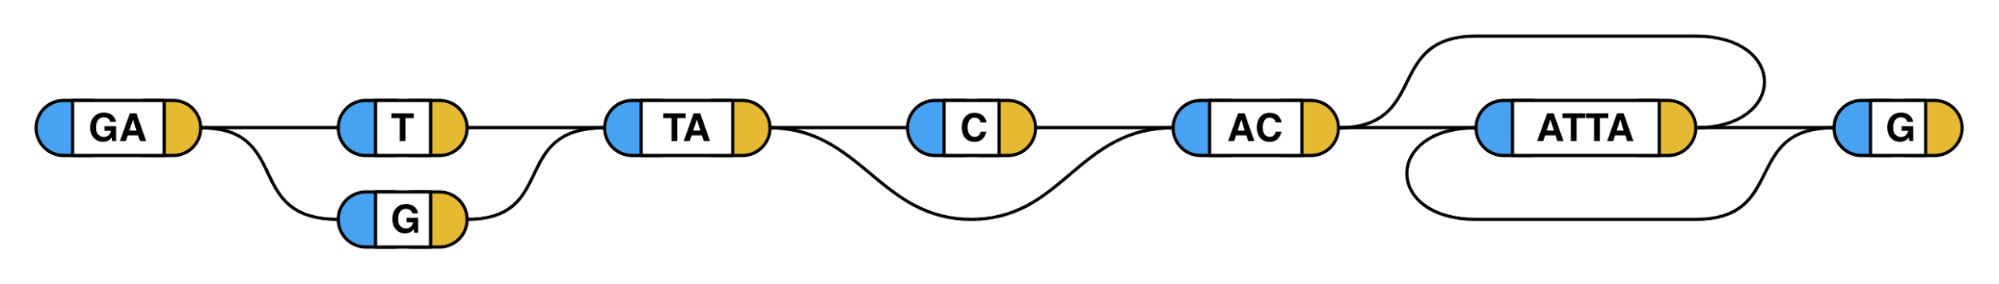
\includegraphics[width=\textwidth]{figures/04_bakeoff/figure01.png}
\caption[Example sequence graphs]{Example sequence graphs. Each node holds a string of bases. An
edge can connect, at each of its ends, to a base on either the left (5',
blue) or the right (3', yellow) side of the node. When reading through a
thread to form a DNA sequence, a valid walk must leave each node via the
opposite side from that through which it was entered; a node's sequence
is read as reverse-complemented if the node is entered on the 3' side.
One thread that this graph spells out (reading from the left side of the
leftmost sequence to the right side of the rightmost sequence, along the
nodes drawn in the middle) is the sequence ``GATTACACATTAG''. Straying
from this path, there are three variants available: a substitution of
``G'' for ``T'', a deletion of a ``C'', and an inversion of ``ATTA''. If
all of these detours are taken, the sequence produced is
``GAGTAACTAATG''. All 8 possible threads from the leading G to the
trailing G are allowed.}
\label{fig:bakeoff:example}
\end{figure}



To evaluate the utility of sequence graphs we invited teams to construct
and evaluate graphs for five test regions of the human genome: the major
histocompatibility complex (MHC), the killer cell immunoglobulin-like
receptors (LRC\_KIR) region, the spinal muscular atrophy (SMA) locus,
and the BRCA1 and BRCA2 genes. MHC, SMA and LRC\_KIR are all regions
with alternate loci represented in GRCh38, while BRCA1 and BRCA2
represent more typical human genes. Regions ranged from 81 kilobases in
size with a single gene (BRCA1) to 5.0 megabases in size with 172 genes
(MHC). We considered graphs from five teams built with eight different
pipelines (Table \ref{tbl:bakeoff:graphs}). For each region we provided a set of long, high
quality input sequences from which to construct graphs (Table \ref{tbl:bakeoff:regions}), but
also encouraged the creation of graphs using additional data of the
builder's choice. Some graphs were built based upon existing variant
calls, such as the 1000 Genomes calls used to construct the 1KG graph
\cite{10002015global}. Graphs were also built
with a wide variety of different algorithmic approaches (Table \ref{tbl:bakeoff:graphs}). Three
control graphs were constructed for each region as points of comparison.
The Primary graphs contain just the single, linear reference path from
GRCh38. The Unmerged graphs consist of just the set of provided
sequences, each represented as a disjoint path. The Scrambled graphs
(see Online Methods) are essentially identical topologically to the 1KG
graphs, but with structures shifted to create false variants. These
graphs acted as a negative control for the effects of adding nonsense
variation to the graphs.

\begin{table}
  \centering
  {\small
  \begin{tabular}{lp{1.5cm}p{1.5cm}p{2cm}p{1.5cm}p{1.5cm}}
  \textbf{Region} & \textbf{Chromo\-some} & \textbf{Length in Primary Reference (bp)} & \textbf{GRCh38 Coordinates} & \textbf{Number of Genes} & \textbf{Alt Haplotypes in pilot data}
  \\
  \hline
  BRCA1 & 17 & 81,189 & 43044293-43125482 & 1 & 2
  \\
  BRCA2 & 13 & 84,989 & 32314860-32399849 & 1 & 2
  \\
  LRC\_KIR & 19 & 1,058,685 & 54025633-55084318 & 47 & 35
  \\
  MHC & 6 & 4,970,458 & 28510119-33480577 & 172 & 8
  \\
  SMA & 5 & 2,397,625 & 69216818-71614443 & 21 & 2
  \end{tabular}
  }

  \caption[Pilot regions]{Pilot Regions. Selected test cases represent
a sampling of both typical and challenging genomic regions.}
  \label{tbl:bakeoff:regions}
\end{table}

\begin{FPtable}
  \centering
  {\small
  \begin{tabular}{p{2cm}p{1.5cm}p{1.5cm}p{5cm}}
  \hline
  \multicolumn{4}{c}{\textbf{Submissions using pilot data}}
  \\
  \hline
  \textbf{Submission} & \textbf{Team} & \textbf{Short Name} & \textbf{Description of Algorithm}
  \\
  \hline
  Cactus & UCSC & Cactus & Graph-based multiple sequence aligner \cite{paten2011cactus2}.
  \\
  Camel & UCSC & Camel & Creates graphs progressively by mapping using
  context schemes \cite{novak2015canonical}.
  \\
  De Bruijn Graph (k=63) & MSKCC & De Bruijn 63 & Forms a De Bruijn graph
  of input data with k=63, then converts to a sequence graph.
  \\
  Population Reference Graph & Oxford & PRG & Creates a graph from a
  K-mer-based HMM description of a region \cite{dilthey2015improved}.
  \\
  Seven Bridges & Seven Bridges & 7BG & Multiple genome alignment.
  \\
  \hline
  \multicolumn{4}{c}{\textbf{Submissions using other data}}
  \\
  \hline
  \textbf{Submission} & \textbf{Team} & \textbf{Short Name} & \textbf{Description of Algorithm}
  \\
  \hline
  1000 Genomes SNP Graph & Sanger/\allowbreak UCSC & 1KG & Generated using vg
  construct on a VCF containing variants identified in the 1000 genomes
  project. Platinum genome samples were not included, to avoid circularity
  in variant evaluation.
  \\
  1000 Genomes Haplotype 50 & Sanger/\allowbreak UCSC & 1KG Haplo 50 & Adapted form of
  1KG graph in which phasing information is used to reduce the number of
  unobserved recombinations represented by the graph. 50~is the number of
  bases two variants can be apart to be considered for this phasing.
  \\
  Scrambled 1000 Genomes & Sanger/\allowbreak UCSC & Scrambled & Generated by shifting
  all the variants in the standard 1KG graph 200~bp downstream.
  \end{tabular}
  }

  \caption[Genome graph submissions]{Genome Graph Submissions. Submissions were collected from a variety of institutions, and showcase a variety of graph construction methods.}
  \label{tbl:bakeoff:graphs}
\end{FPtable}

\begin{FPfigure}
\centering
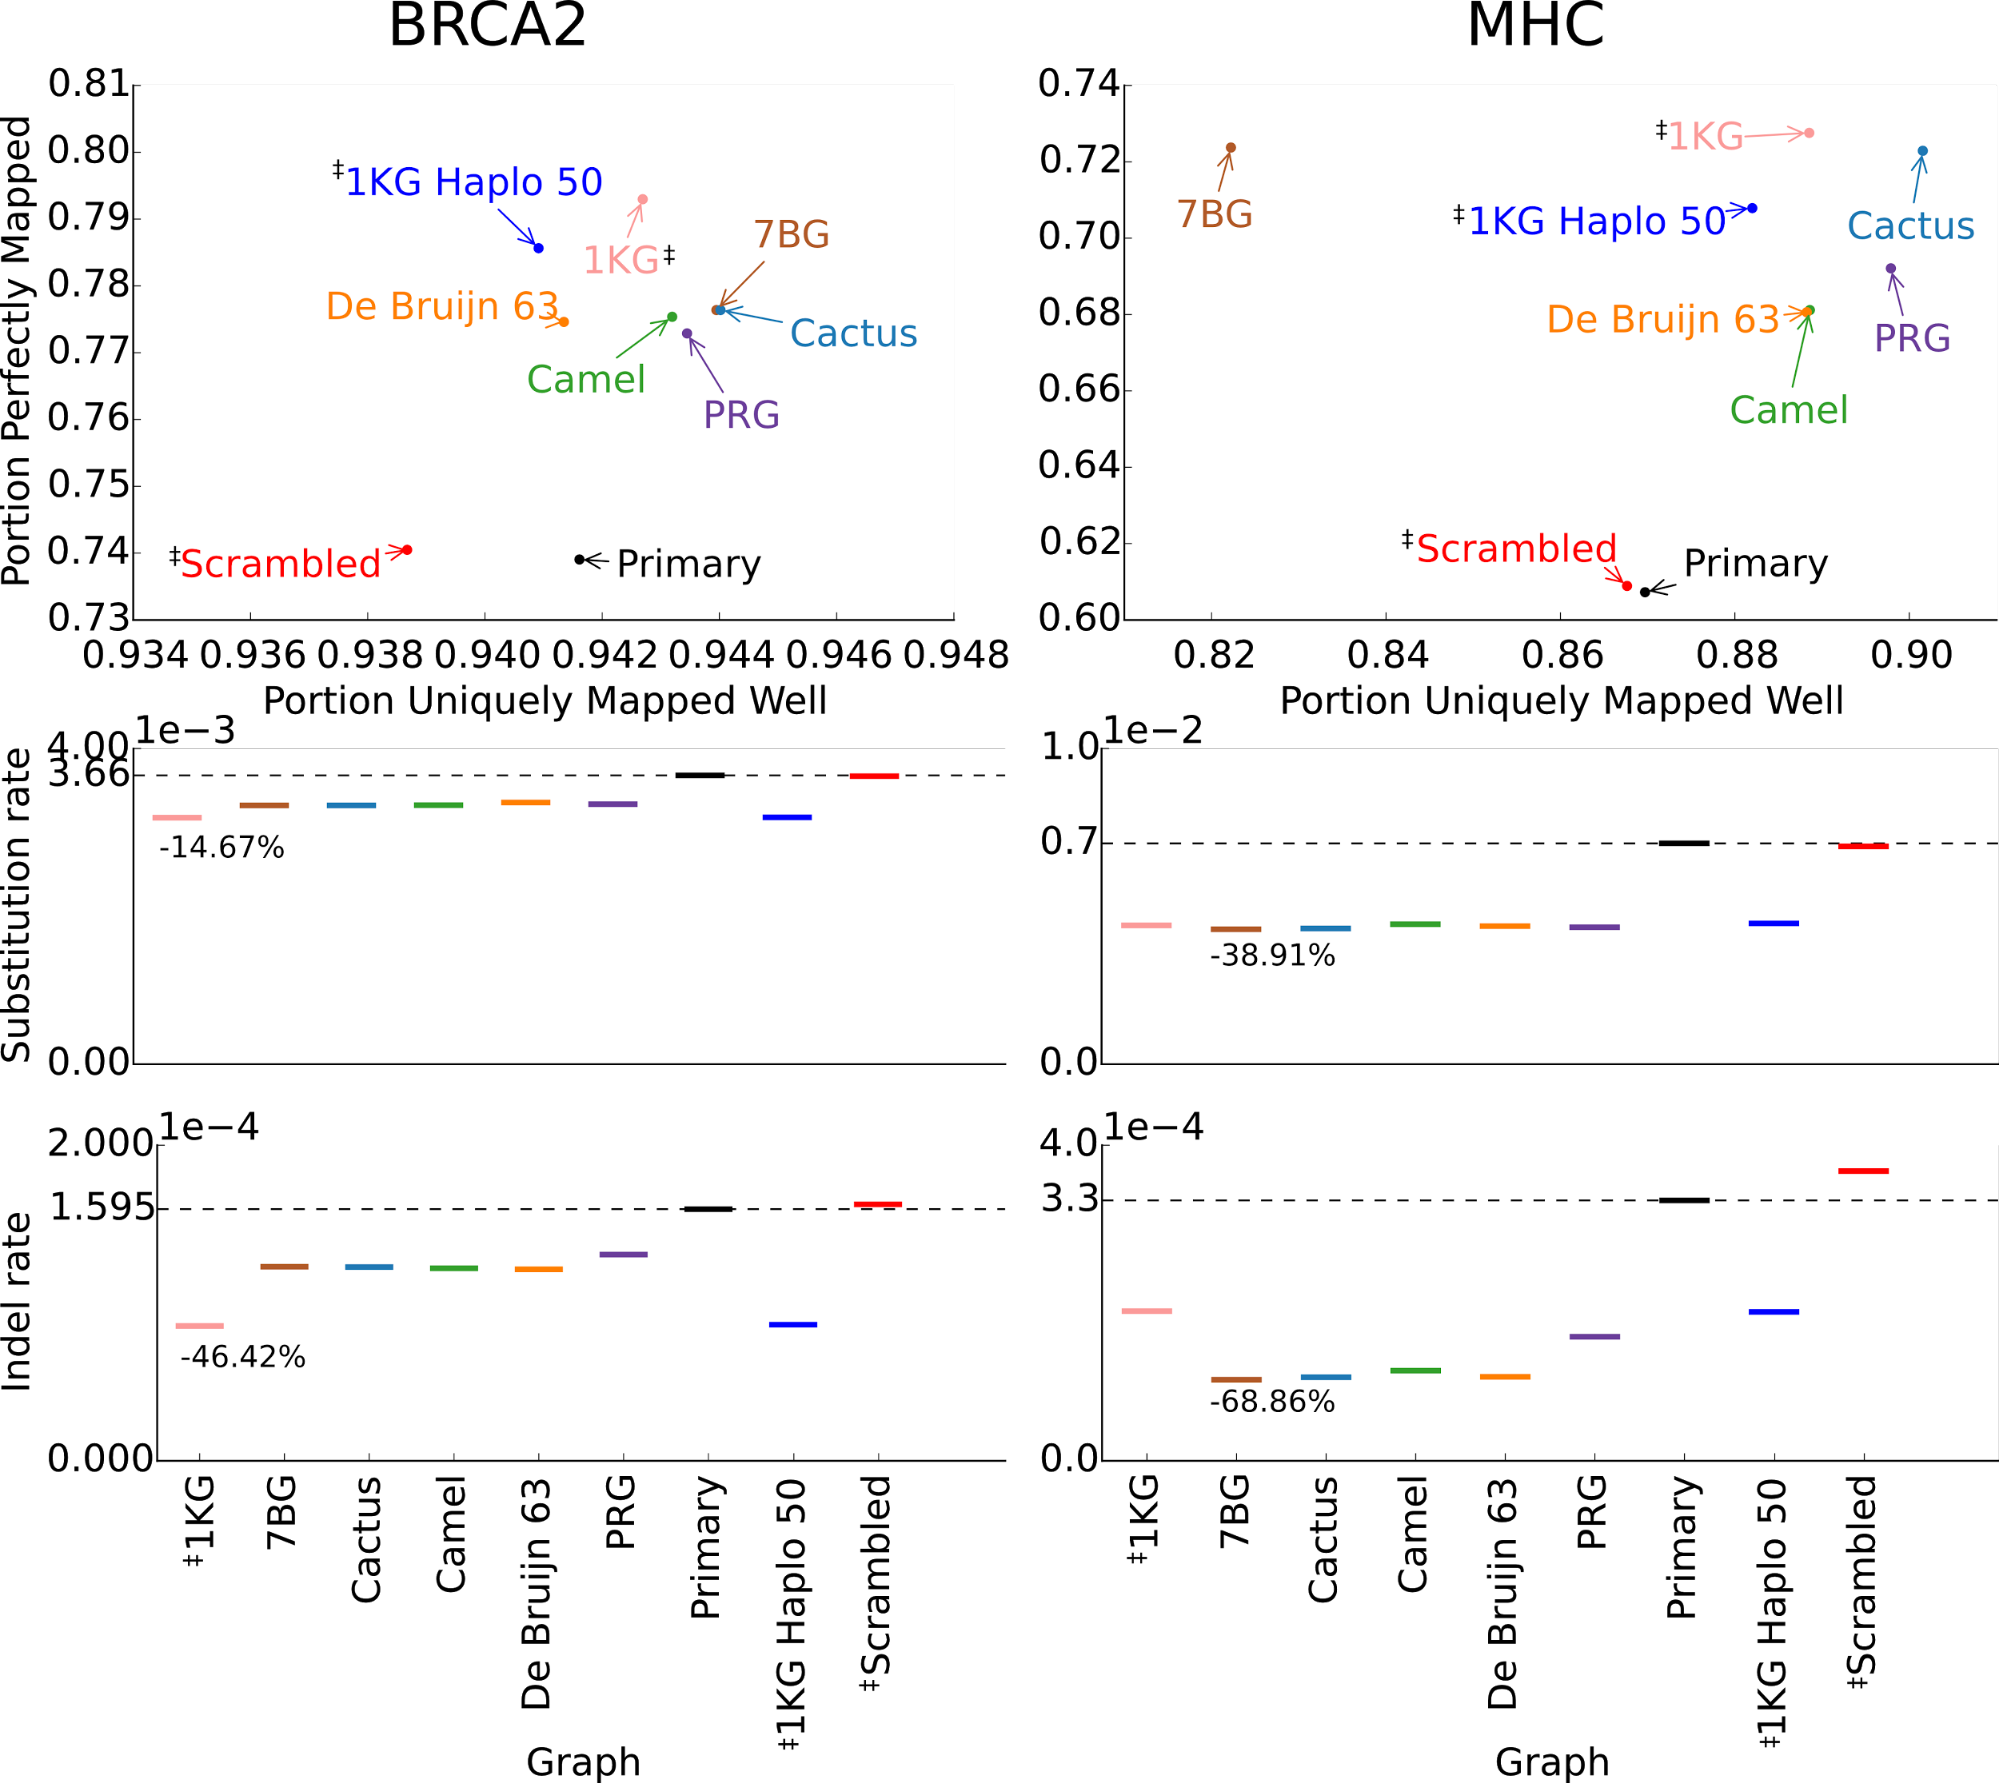
\includegraphics[width=\textwidth]{figures/04_bakeoff/figure02.png}
\caption[Mapping reads to sequence graphs]{Mapping reads to sequence graphs. Results for the 1000 Genomes
Phase 3 low coverage samples against the BRCA2 and MHC graphs. The
median per-sample portion of reads that are mapped perfectly (Y axis),
and the median per-sample portion of reads that are mapped with a
unique, obviously-best alignment (X axis) are both visible in the top
row. The median per-sample substitution rate for a primary mapping,
computed per aligned base, is shown in the second row. The median per
sample frequency of indels in primary mapped reads, computed per read
base, is given in the third row. The horizontal black line represents
the result for the primary reference graph in the region. The ‡ symbol
marks graphs generated using additional data beyond the provided
reference and alternate sequences. The unmerged graphs are excluded
because very few reads mapped uniquely to them.}
\label{fig:bakeoff:mapping}
\end{FPfigure}

\subsection{Graph Read Mapping}

To evaluate the utility of sequence graphs for read mapping we used the
software program vg\cite{Vgteam_undated-xe}, which contains a mapping
algorithm capable of mapping to a fully general and potentially cyclic
sequence graph (see Supplementary Section 2). We mapped all relevant
reads (see Online Methods) from 1000 Genomes Phase 3 low coverage
samples to each graph. We found that vg was able to map almost all such
reads to the graphs (Supplementary Fig. 3).

Relative to the primary graph, a graph containing more of the variants
should produce an increase in the fraction of reads that map perfectly
(without either substitutions or indels) to at least one place. For
BRCA2 we see a relative increase of 7.3\% in the median number of reads
mapping perfectly to the 1KG graph vs.~the Primary graph, but for MHC
the increase is 20\% (Fig. \ref{fig:bakeoff:mapping} top row, Supplementary Section 3,
Supplementary Fig. 1). The increase for BRCA2 is close to what would be
expected if the sequence graph contained the majority of polymorphisms
for a typical region of the genome (Supplementary Section 3), while the
larger increase for MHC is likely due to a greater degree of
polymorphism \cite{brandt2015mapping}. Similar, slightly smaller increases
are seen for graphs built from other, smaller collections of variants.
The scrambled graphs do not show significant gains, thus indicating that
the effect is specific to graphs containing known variation.
Furthermore, the overall substitution rate between reads and the
experimental graphs was observed to decrease, relative to the rate
between the reads and the Primary control graph. In the
highest-performing graphs the decline is slightly below the bounds of
previous read substitution error rate estimates of 0.7-1.6\%
\cite{Minoche2011-il,1000_Genomes_Project_Consortium2010-ky,1000_Genomes_Project_Consortium2012-gr,10002015global}
(Fig. \ref{fig:bakeoff:mapping} second row; see Supplementary Section 4 and Supplementary Fig.
4). The decrease in indel rate (Fig. \ref{fig:bakeoff:mapping} third row) moving from the
Primary graph to the 1KG graph is comparable to estimates of the human
indel polymorphism rate\cite{Mills2011-lj} (Supplementary Section 5).

The median fraction of reads that uniquely map increases for many of the
graphs, relative to the primary and scrambled graphs. For example, in
the Cactus graph, an increase of 0.26\% is observed in BRCA2, and an
increase of 3.7\% is observed in the MHC. No such increase in unique
mapping is seen for the comparably complex scrambled graph. Unique
mapping is defined as having a good primary mapping and no reasonable
secondary mapping (see Supplementary Section 3 and Supplementary Fig.
2).

To test if the choice of sequence graph reference affected population
level reference allele bias, we binned samples by 1KG super-population
and looked at the difference in perfect mapping between the 1KG graph
and the Primary graph for each subpopulation. We find a small but
significant difference in perfect mapping increase between
super-populations for most regions (Supplementary Section 6,
Supplementary Fig. 5), but we also find relatively large differences in
absolute rates of perfect mapping (Supplementary Fig. 6). These latter
differences suggest that super-population may be confounded with
sequencing batch, making drawing conclusions from this analysis quite
difficult.

\subsection{Graph Variant Calling}

We implemented a comprehensive, albeit basic, variant calling pipeline
based on the Samtools pileup approach \cite{Li2009-je}, modified to work
with sequence graphs (see Online Methods for more details). In summary
(Fig. \ref{fig:bakeoff:calling}), reads are mapped to the reference graph or \emph{base graph}
and a pileup is computed at each graph position and edge. An
\emph{augmented} \emph{graph} is created by extending the base graph
with additional sequences and edges representing possible variants
determined from the pileups. This graph is then analyzed for
\emph{ultrabubbles} (acyclic, tip-free subgraphs connected to the rest
of the graph by at most 2 nodes) which are treated as sites for
genotyping\cite{paten2017superbubbles}. Finally, thresholding heuristics
are used to emit a set of genotypes with sufficient read support, one
for each site, expressed in the coordinates of the GRCh38 primary
reference path as embedded in the graph (see Online Methods).

\begin{FPfigure}
\centering
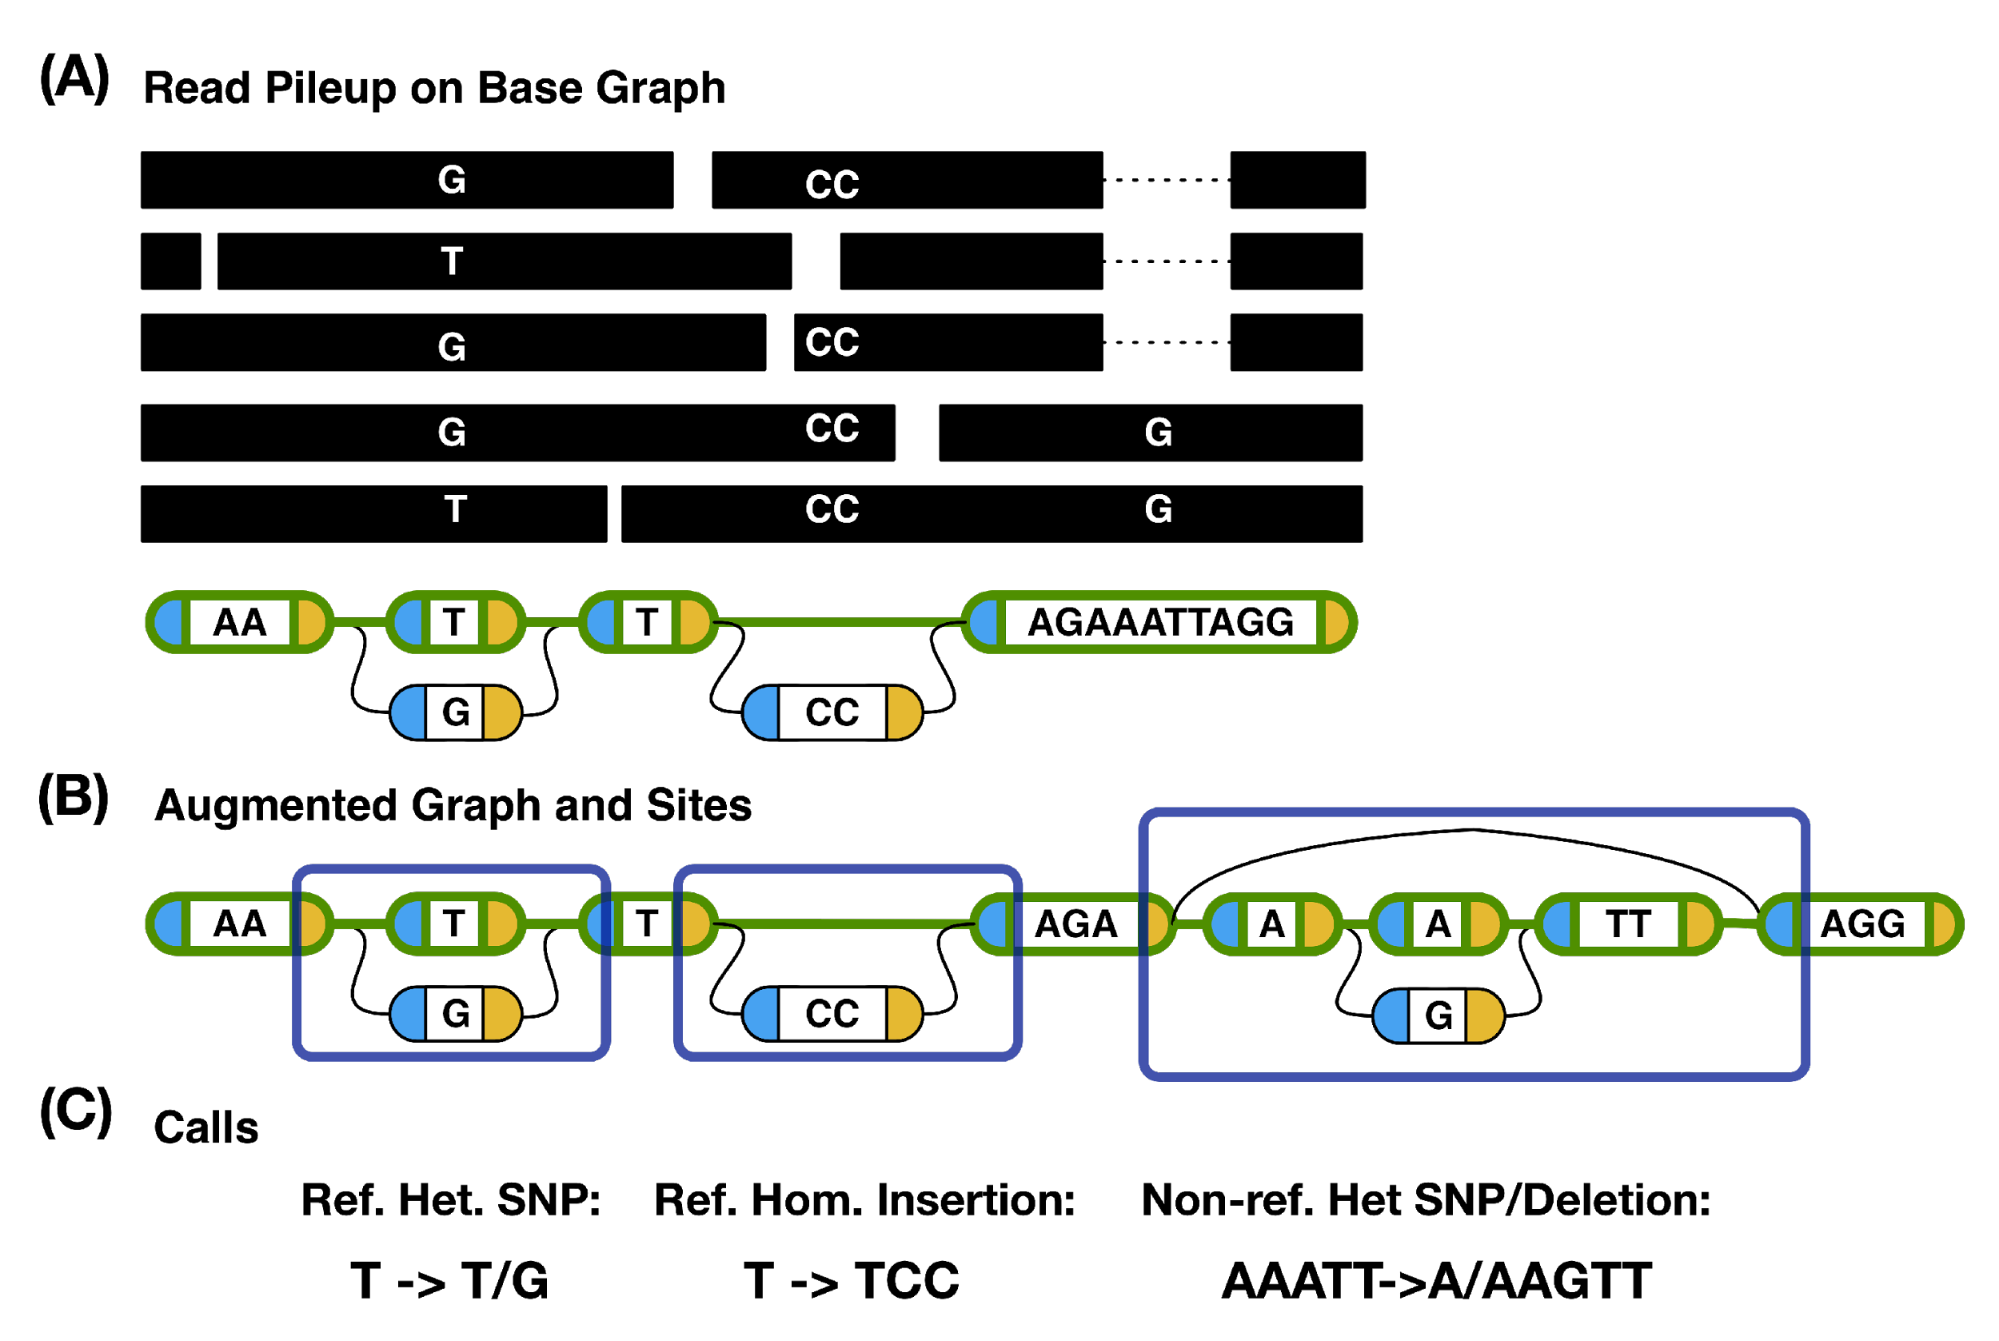
\includegraphics[width=\textwidth]{figures/04_bakeoff/figure03.png}
\caption[Variant calling with genome graphs]{Variant Calling with Genome Graphs. (A) Read pileup on a base
graph whose reference path is highlighted in green. Only variant or
non-reference base values are shown in the reads. (B) The augmented
graph contains the base graph as well as new structures implied by the
pileup. This graph contains three top-level ultrabubbles, each forming a
site. (C) Variant calls for each site. The first two (a heterozygous SNP
and a homozygous insertion) are considered reference calls because they
were present in the base graph, whereas the third (a heterozygous
combination of a SNP and a deletion) is non-reference because it was
novel to the augmented graph.}
\label{fig:bakeoff:calling}
\end{FPfigure}

We compared the results from the graph variant calling pipeline with the
Platinum Genomes benchmark data for samples NA12877 and
NA12878\cite{Eberle2016-zc} using vcfeval, which corrects for VCF
representation ambiguity by comparing at the haplotype level
\cite{Cleary2015-oy} \cite{Zook2014-tl}. To provide additional controls,
Freebayes \cite{garrison2012haplotype}, Platypus \cite{Rimmer2014-zj} and
Samtools \cite{Li2009-je} were run on BWA-MEM \cite{li2009fast}
alignments of the same input data to GRCh38 with their default options
in order to produce positive control variant calls. Figure \ref{fig:bakeoff:callingeval} (A) shows
the precision and recall of each method aggregated across both samples
and all regions. Figure \ref{fig:bakeoff:callingeval} (C) and (D) show precision-recall curves for
SNPs and indels, respectively. In comparison to the primary graph (the
graph containing only the existing reference sequence, and therefore a
control for the same variant calling algorithm applied to just the
knowledge in the existing reference), the 1KG and Cactus graphs'
F1-scores (Supplementary Table 1) increased by 3.50\% and 1.98\%,
respectively, increasing for both single nucleotide variants (3.13\%,
1.95\% respectively) and indels (6.02\%, 4.40\% respectively).
Furthermore, 1KG graphs have the overall highest accuracy (F1 score) of
all methods, although Samtools and Platypus perform best overall for
SNPs and indels, respectively. Supplementary Section 7 contains
additional breakdowns of the F1-scores by region (Supplementary Figs.
7-8), sample (Supplementary Fig. 9), and type (Supplementary Fig. 10),
as well as scores without clipping to confident regions (Supplementary
Fig. 11). Generally (in 13 out of 18 cases), the 1KG graph has higher
accuracy than both the primary and scrambled controls.

We define a \emph{reference} \emph{call} as a call asserting the
presence of a position or edge in the base graph. The experimental
graphs can dramatically reduce the number of non-reference calls, as
compared to control. For example, the Cactus and 1KG graphs reduce
non-reference calls by more than a factor of ten (Fig. \ref{fig:bakeoff:refnonref} (A)) relative
to the Primary reference graph. Furthermore, the precision of these
reference calls is higher than the non-reference calls for the
non-scrambled graphs (Fig. \ref{fig:bakeoff:refnonref} (B)).

Larger structural variants can be called using the same logic as point
mutations, provided they are already in the graph; Figure \ref{fig:bakeoff:refnonref} (C) displays
the indel length distribution for the two top-performing graphs and the
primary control, as well as a breakdown of indel lengths for reference
and non-reference calls. The reference call indel lengths in the
experimental graphs are larger than the Primary and non-reference
lengths and, in the case of Cactus, contain indels exceeding the read
length. This adds up to a large number of additional called bases: for
example, across the regions the Cactus graphs call 94 indel events
larger than 50 base pairs totaling 10045 bases, none of which are found
using the Primary graph with the same algorithm.

To mitigate potential biases with the Platinum Genomes benchmark data as
a truth set\cite{Eberle2016-zc}, we conducted what we term a
``reference-free'' evaluation of vg's variant calling accuracy, by
comparing against de novo assemblies instead of assumed-true variant
calls. In brief, short reads pooled from two haploid assemblies were
used to call variants on each sequence graph. The accuracy of this
reconstruction was evaluated using PacBio-based \emph{de novo} assembly
fragments, which by definition are free of reference artifacts and are
derived from a different sequencing technology (see Online Methods,
Supplementary Section 8 and Supplementary Figure 12). The results can be
seen in Figure \ref{fig:bakeoff:callingeval} (B) and Supplementary Figure 13. Several experimental
graphs have greater precision and recall than the Scrambled and Primary
controls; combined across all regions except SMA (which was
insufficiently covered by PacBio assemblies to be usefully analyzed), vg
on the Cactus graph outperformed existing methods. The results appear to
agree closely with those from the VCF-comparison-based evaluation,
considering that the two techniques use different sources of truth and
different evaluation metrics.

\begin{FPfigure}
\centering
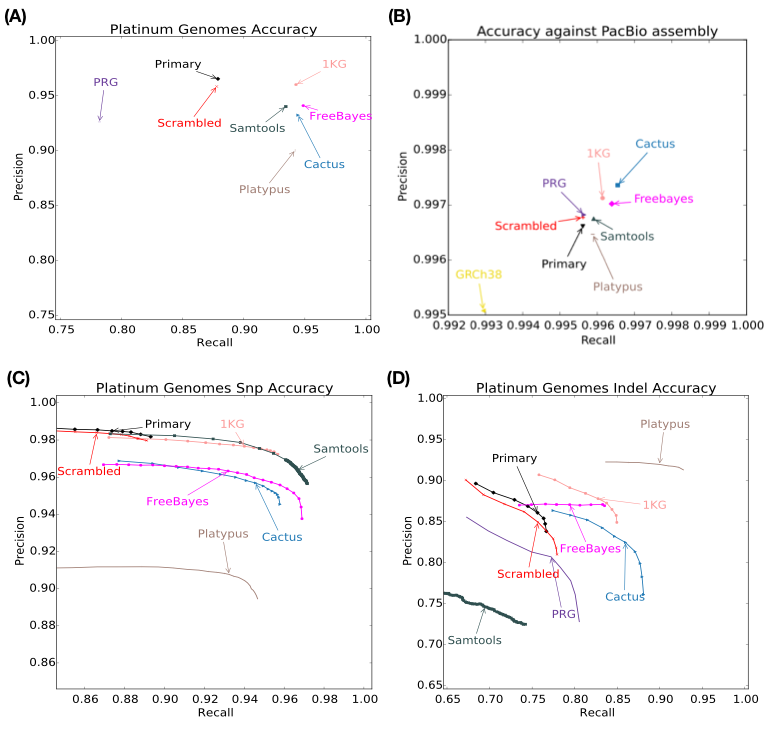
\includegraphics[width=\textwidth]{figures/04_bakeoff/figure04.png}
\caption[Variant calling evaluation]{Variant Calling Evaluation. (A) Precision (portion of called
variation in agreement with the truth set) and recall (portion of
variation in the truth set in agreement with what was called) against
the Platinum Genomes truth VCFs aggregated across NA12877 and NA12878
for all regions, as measured by vcfeval. (B) Per-base precision and
recall as measured by the reference-free evaluation in BRCA1, BRCA2,
LRC\_KIR, and MHC. The GRCh38 point shows a comparison of the existing
primary reference haplotype sequence against the de novo assembly. (C) -
(D) Breakdown of precision and recall from (A) into SNPs and indels,
respectively. Curves are shown by including accuracies at quality
thresholds that fall within a radius of 0.1 around the maximum F1. Full
results featuring F1-scores for all graphs are in Supplementary Section
7.}
\label{fig:bakeoff:callingeval}
\end{FPfigure}

\begin{figure}
\centering
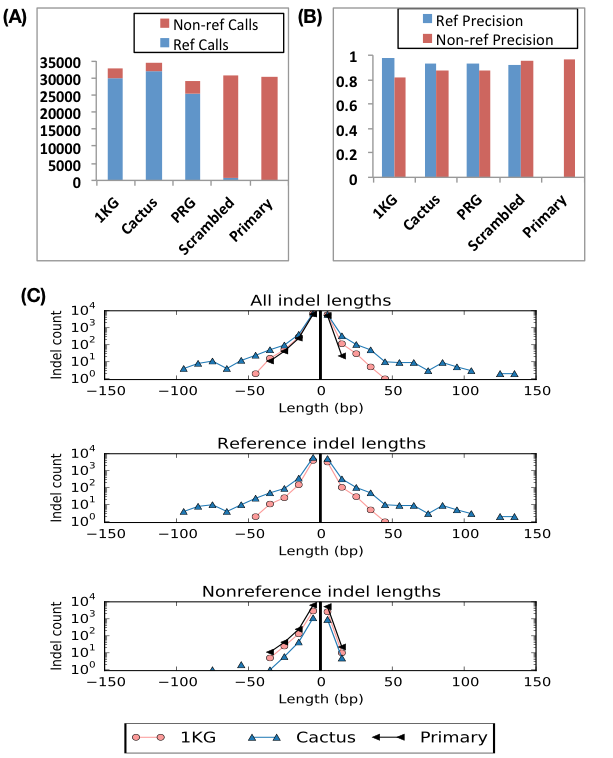
\includegraphics[width=2in]{figures/04_bakeoff/figure05.png}
\caption[Reference versus non-reference calls]{Reference versus Non-reference Calls. (A) Total number of
reference and non-reference calls across all samples and regions. (B)
Precision of reference and non-reference calls. (C) Indel lengths of
reference and non-reference calls, where insertions and deletions are
represented by positive and negative lengths, respectively. In all cases
we ignore calls of GRCh38 reference alleles, as these numbers are
reported from GRCh38-based output VCFs.}
\label{fig:bakeoff:refnonref}
\end{figure}

\subsection{Short Path Accuracy}

We sought to understand how complete and accurate the sequence graphs
studied were in their representation of common variants. To approximate
this, we measured the fraction of lightly error-pruned K-mer instances
(here K=20, see Online Methods) in a large subset of 1KG sequencing
reads that were present within each graph, calling this metric
\emph{K-mer recall} (see Online Methods). We observe (Fig. \ref{fig:bakeoff:shortpaths},
Supplementary Section 9, and Supplementary Fig. 14) that graphs built
from the largest libraries of variation contain the great majority of
such K-mer instances. For example the 1KG, PRG and Cactus graphs contain
an average across regions of 99\% of K-mer instances, while the primary
graph contains an average across regions of 97\%. Conversely, we asked
what fraction of 20-mer instances present in a graph were not present in
any 1KG read, calling this metric \emph{K-mer precision}. Strikingly, we
find that precision is greatly reduced in some graphs relative to
control. For example around 15\% (averaged across regions) of 20-mers
enumerated from 1KG graphs do not appear in any 1000 Genomes low
coverage read. We hypothesize that this is because the density of
variation is sufficient in such graphs to admit many paths implying
recombinations that are either absent or very rare in the population. To
attempt to raise precision, for the 1KG data we constructed graphs using
haplotype information to eliminate a substantial subset of unobserved
paths, creating the ``1KG Haplo 50'' graph (Supplementary Section 10).
This resulted in increased precision (by about 10 percentage points in
BRCA2) with only a small reduction in recall, as shown in Figure \ref{fig:bakeoff:shortpaths} and
Supplementary Figure 13. However, this comes at the cost of a
performance degradation in read mapping (Fig. \ref{fig:bakeoff:mapping}) and variant calling
(Supplementary Section 7). One possible explanation for the performance
reduction is that the necessary duplication (``unmerging'') of paths in
this procedure reduced the aligner's ability to unambiguously map reads.

\begin{figure}[htbp]
\centering
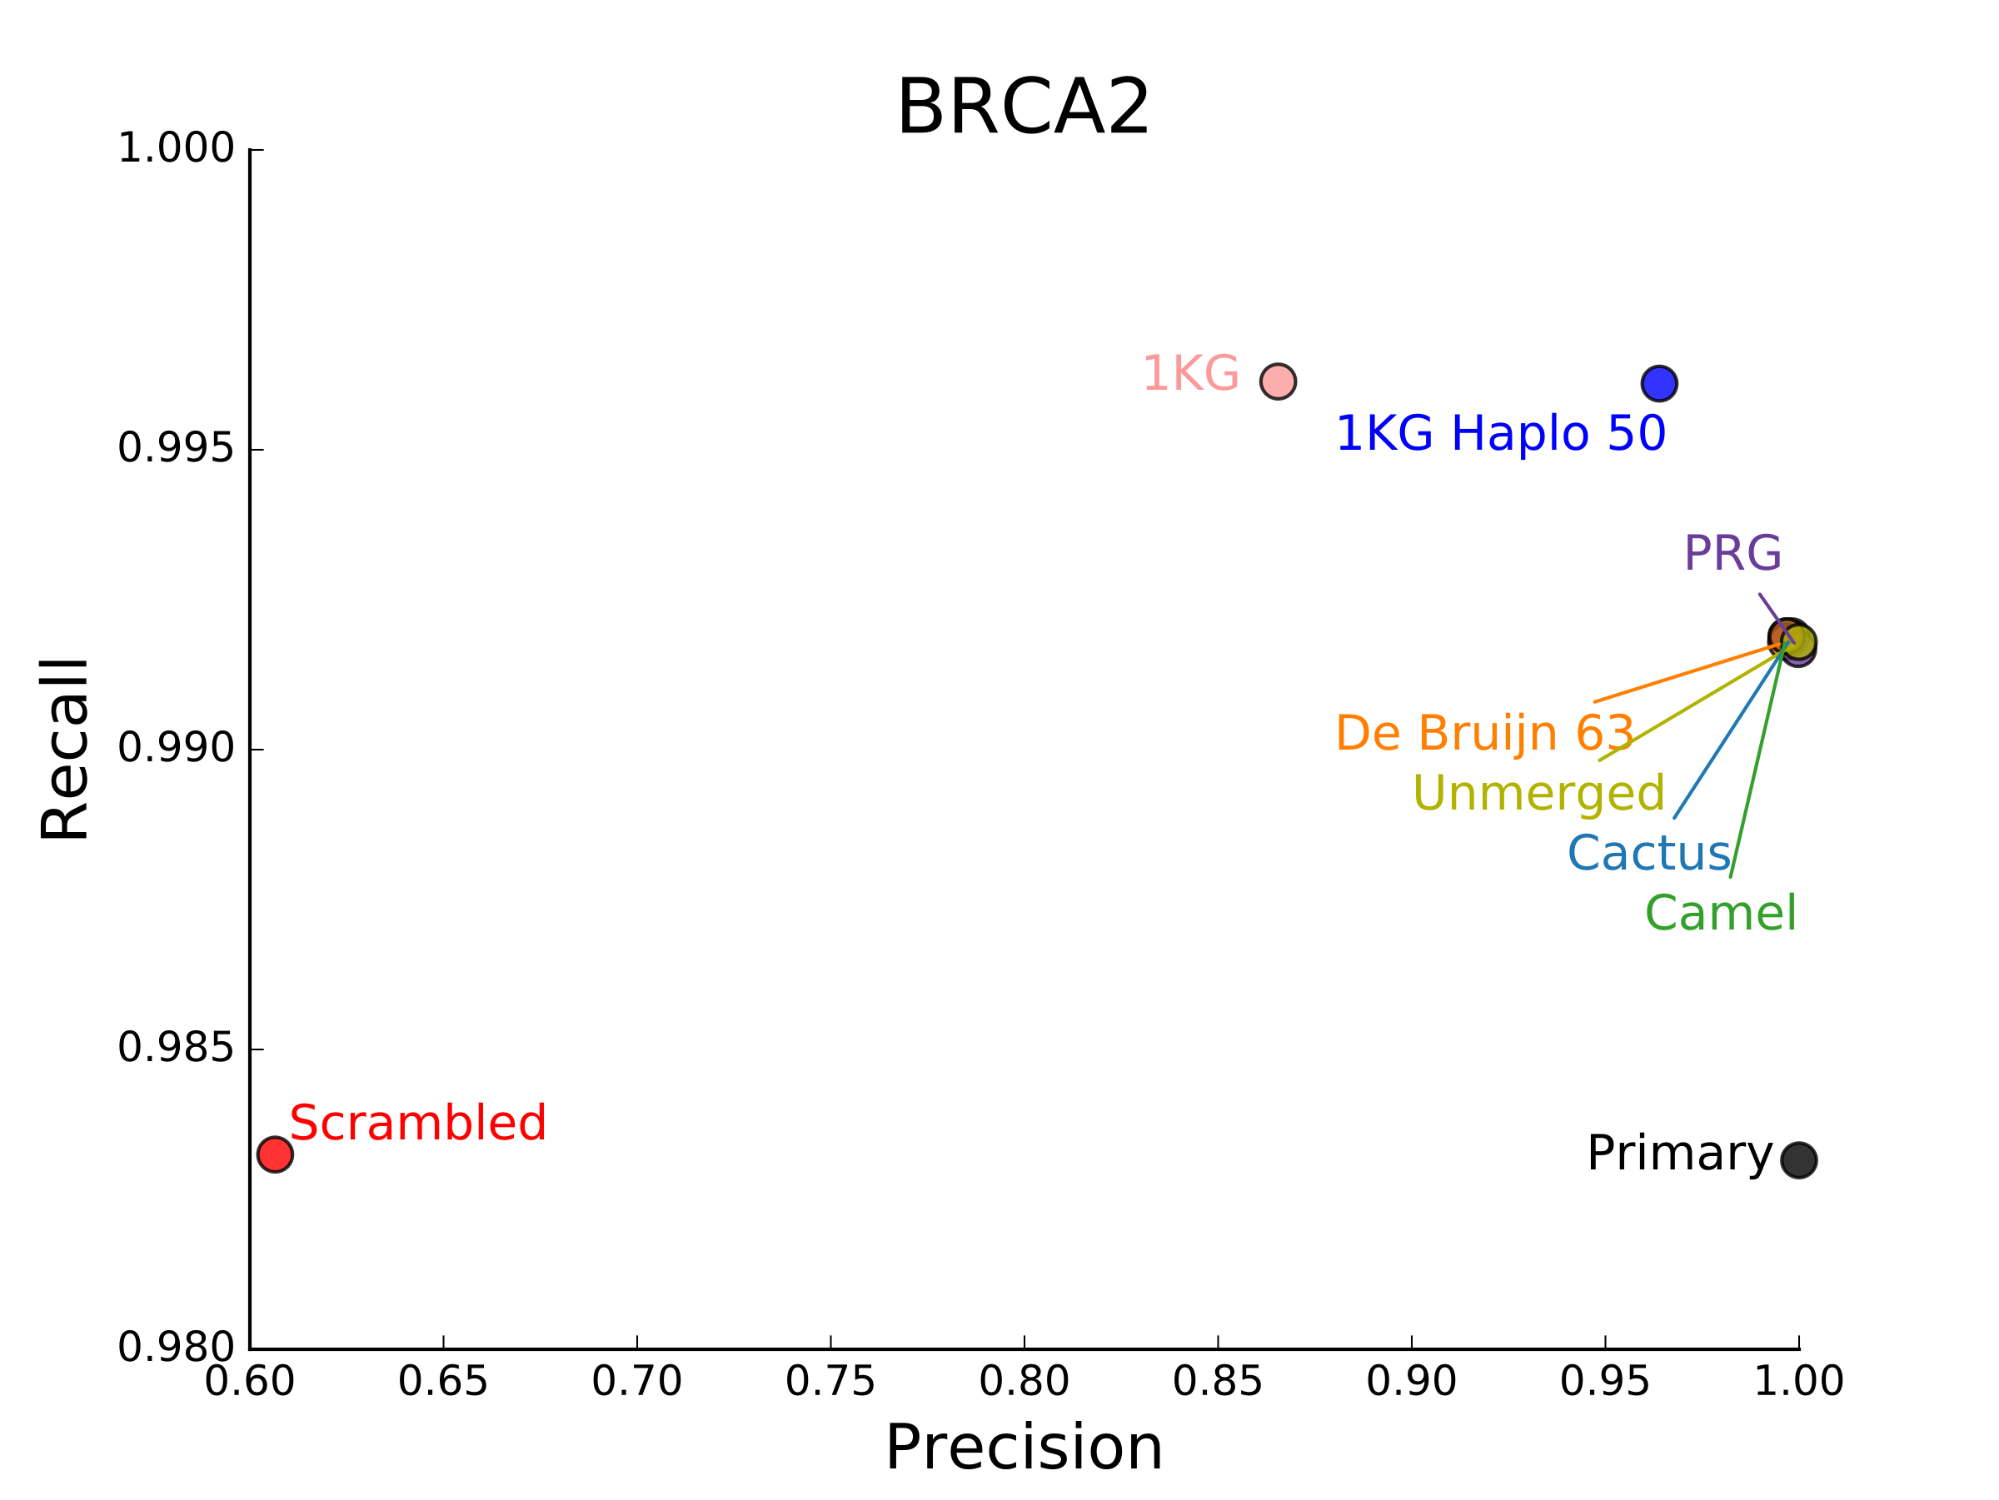
\includegraphics[width=0.5\textwidth]{figures/04_bakeoff/figure06_1.png}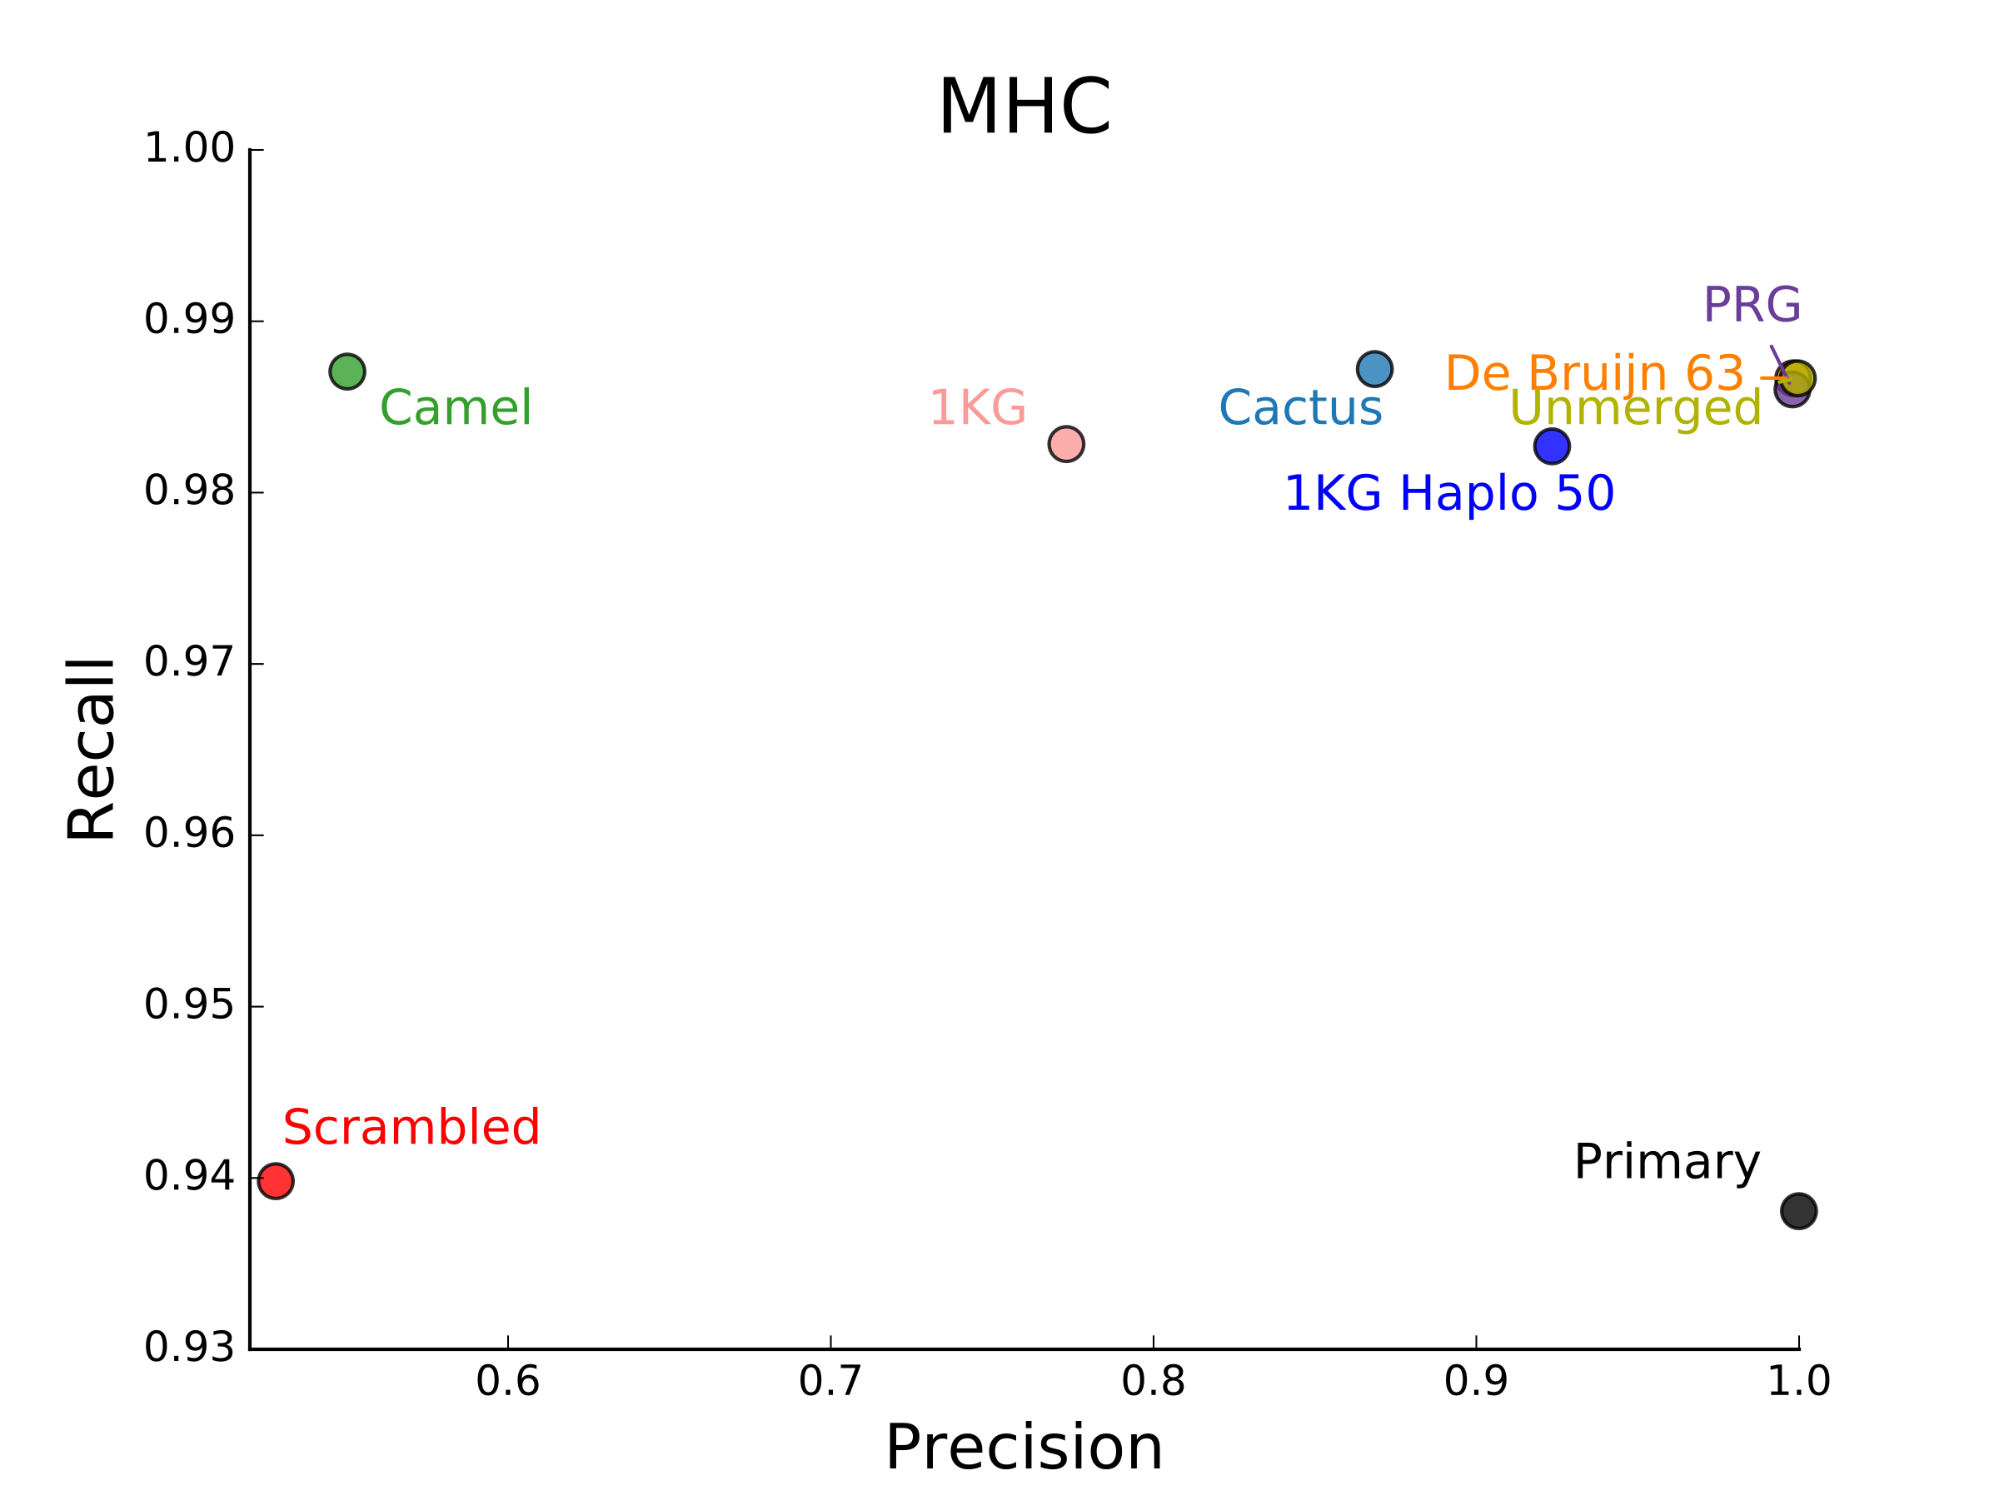
\includegraphics[width=0.5\textwidth]{figures/04_bakeoff/figure06_2.png}
\caption[Short path completeness and accuracy]{Short path completeness and accuracy. Assayed by comparing
20-mer instances.}
\label{fig:bakeoff:shortpaths}
\end{figure}

\subsection{Graph Character}

We found that even within each region the different submitted graphs
varied substantially in their performance on our evaluations of read
mapping and variant calling. They varied even more so with respect to
basic graph properties (Supplementary Section 11, Supplementary Tables
2-9). To quantify this variability we defined normalized graph metrics
for basic graph properties. \emph{Graph compression} is the length of
the primary reference sequence within the region divided by the sum of
the lengths of the nodes in the graph. It is a normalized measure of the
number of positions in the graph. The \emph{(base) degree} is the average
per-side degree of the graph in a bidirected graph representation with
single-base nodes, and is a measure of how much branching a graph
contains. The \emph{cut width} (Supplementary Table 10) is a measure of
apparent sequence rearrangement. Briefly, within a topologically sorted
graph, where all positions are ordered, cut width is the average over
all gaps between successive positions of the number of edges connecting
positions on the left side of the gap to positions on the right side of
the gap (Supplementary Section 12)\cite{haussler2017flow}. We see
wide variation in these measures across the graphs (Fig. \ref{fig:bakeoff:graphstats}).
Furthermore, across the different regions we find that there is an
inverse correlation (R=-0.674, p=0.00230) between cut width and variant
calling accuracy and a positive correlation (R=0.244, p=0.0268) between
compression and variant calling accuracy (Supplementary Fig. 15). The
base degree does not significantly correlate with variant calling
accuracy. These correlations suggest that uncompressed and highly
rearranged graphs do not work effectively with our current read mapping
and variant calling process.

\begin{FPfigure}
\centering
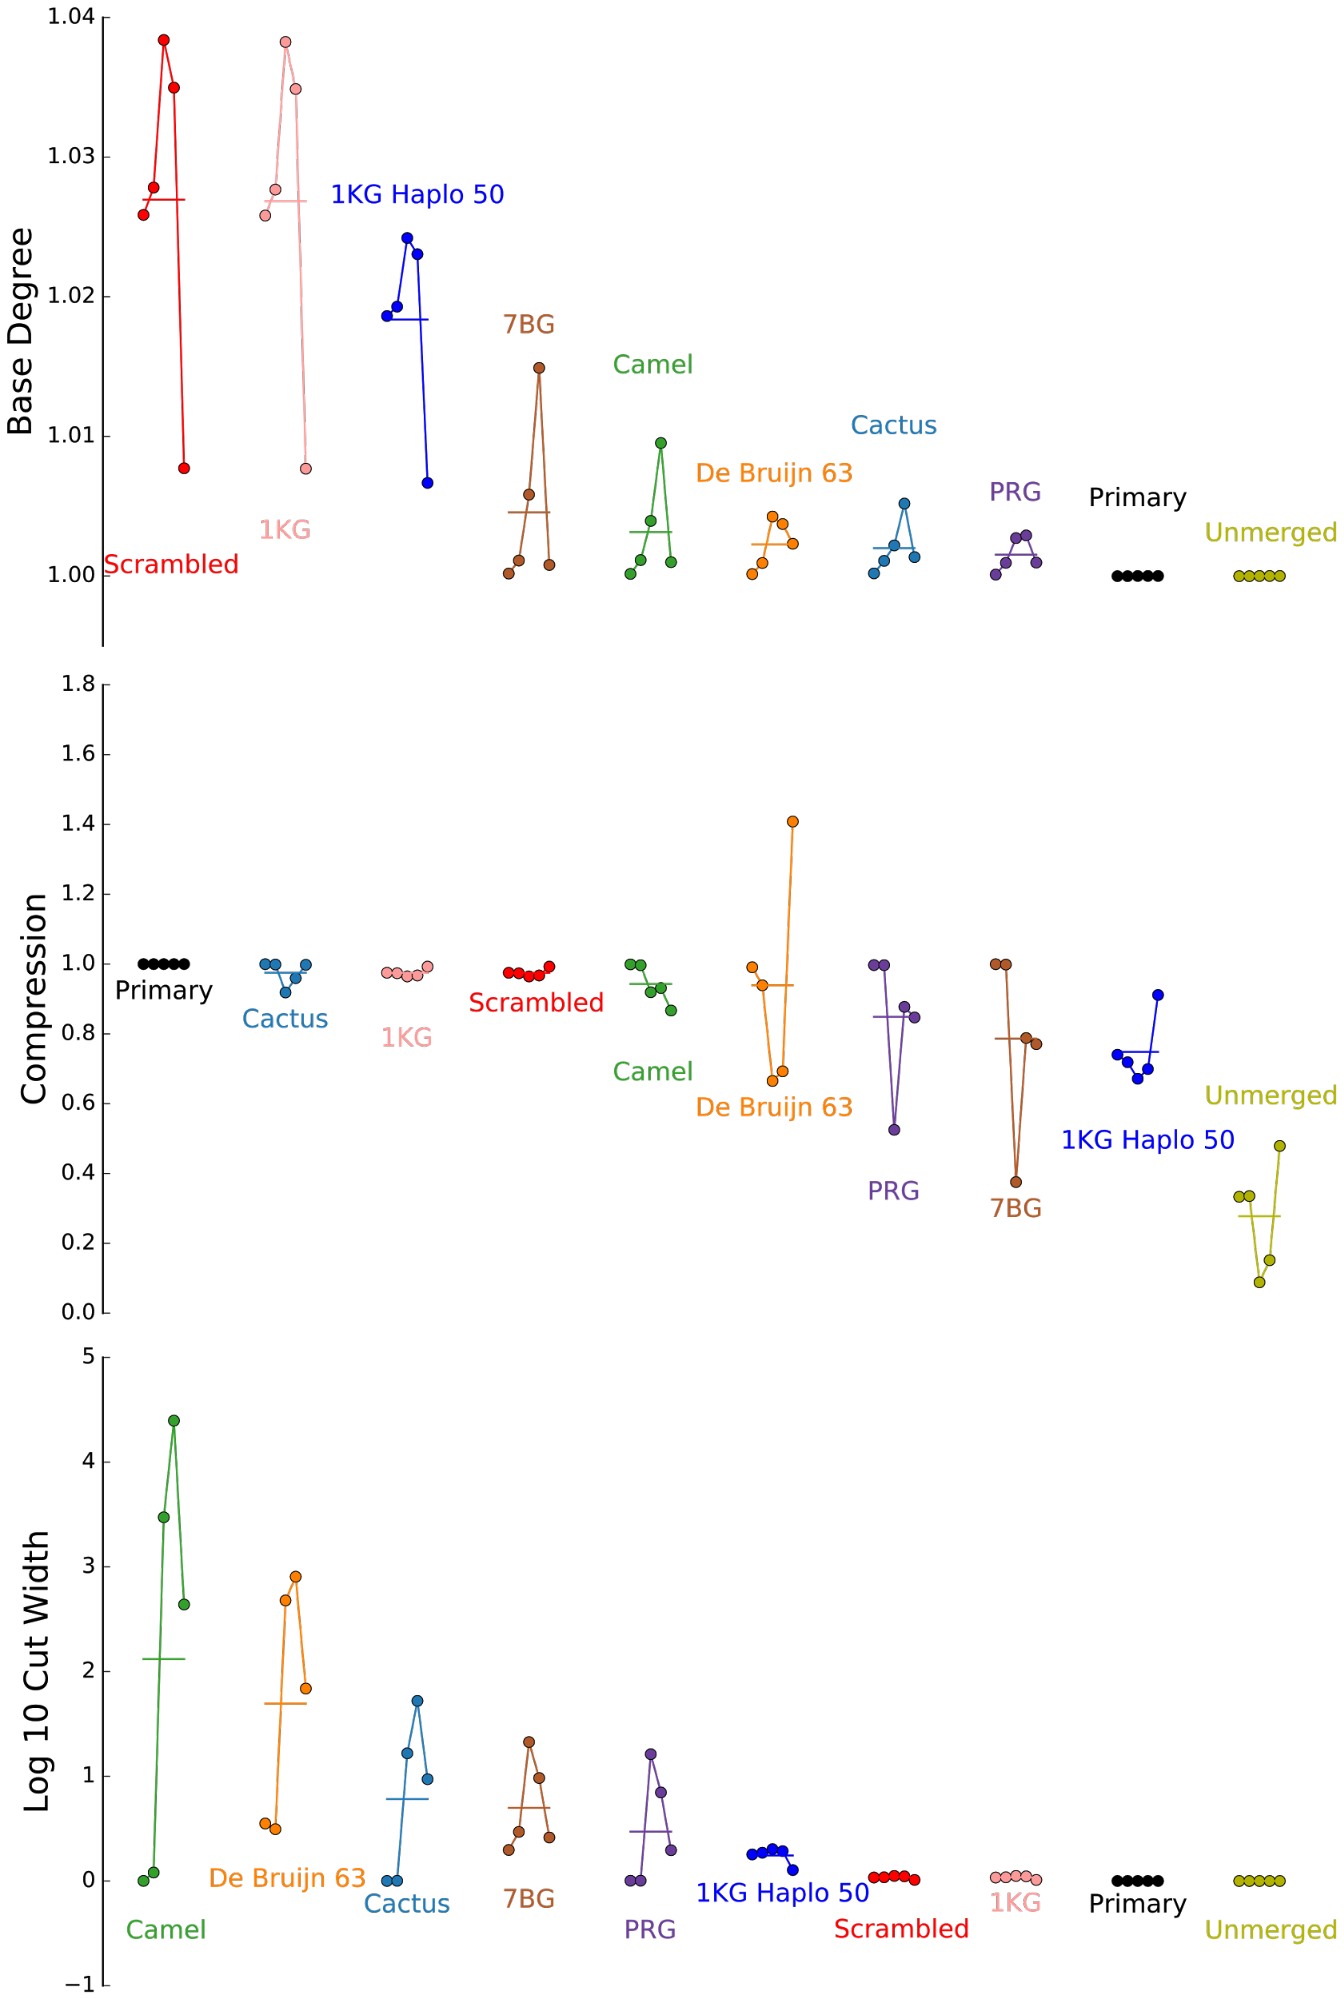
\includegraphics[width=0.9\textwidth]{figures/04_bakeoff/figure07.png}
\caption[Empirical graph statistics]{Empirical graph statistics. In each panel the result for each
region is shown by a dot, in the following order: BRCA1, BRCA2,
LRC\_KIR, MHC, and SMA.}
\label{fig:bakeoff:graphstats}
\end{FPfigure}

\section{Discussion}

Contemporary non-graphical variant calling procedures use different
algorithms for each class of variants: substitutions, small indels,
larger indels, balanced rearrangements, and so on. We have demonstrated
that variant calling on a sequence graph mostly obviates this
complexity, because being able to call the presence or absence of
elements within a sample graph is potentially sufficient for calling
known structural and point variation equally well. The simple, nascent
variant calling algorithm we tested produced variant calls that were
quite concordant with those from other state-of-the-art variant calling
pipelines, while unifying the calling of known SNPs and other known
structural variation. That individual tools slightly outperformed the
variant calling algorithm presented here in terms of individual variant
types, i.e.~snps and indels, is unsurprising given the relative maturity
and algorithmic sophistication of those tools. Importantly, many of the
submitted graphs showed improved variant calling performance over the
primary and scrambled graphs. The relative improvements come alongside a
large reduction in the number of non-reference calls. Furthermore,
reference calls were more accurate than non-reference calls, suggesting
that variant calling is indeed more accurate overall when the variants
themselves are contained within the graph. These results support the
notion that sequence graphs can transform variant calling by reducing it
to the simpler problem in which only rare variants, absent from the
graph, must be discovered de novo. It is possible to foresee cutting the
number of non-reference point variation calls from the millions, as in
standard genome wide pipelines today, to on the order of thousands (see
Supplementary Section 3).

During the course of the variant calling comparison, we developed an
appreciation for the shortcomings of relying solely on the Platinum
Genomes benchmark data as a truth set\cite{Eberle2016-zc}. A key concern
is that the Platinum Genomes calls were derived by means of a consensus
of contemporary methods, all of which use the existing linear reference
and BWA-MEM-based mappings. Additionally, compared to vg, the Platinum
Genomes dataset often uses different combinations of calls to ``spell''
the same haplotype. Moreover, it often omits calls necessary to spell a
haplotype because it is not confident in them. While the omitted calls
are in regions marked as low confidence, a variant normalizer cannot
normalize a call that is not there. To get around these problems and
potential biases we introduced a reference-free method for assessing
variation calls. This evaluation demonstrated good consistency with the
Platinum Genomes in terms of the relative ranking of the different
methods evaluated, and demonstrated clearly that the best graph methods
slightly outperform existing methods.

Supporting the observed improvements in variant calling, we demonstrate
that read mapping can be made both more comprehensive and less ambiguous
with sequence graphs. Increases in perfect mapping and reductions in
substitution and indel rates were broadly consistent with the effect we
would expect if the graphs were representing the majority of common
polymorphisms, leaving the residual read error rates to account for the
majority of alignment differences. In this sense read mappings were
demonstrated to be less locally ambiguous, with mismatches and edits
having a more clearly defined meaning. Furthermore, the fact that read
mappings were also less globally ambiguous (i.e.~more certain in their
overall placement within the genome) is perhaps surprising. We thought
at the outset that using detailed graphs would have the drawback of
increasing the number of times a read maps to two or more places by
increasing the sheer number of mapping possibilities. However, we found
that the opposite is true - the addition of known polymorphisms to the
graph allows reads to better distinguish their true mapping location
from secondary, paralogous locations. Scaled genome-wide, these
improvements could help canonicalize mapping to the vast majority of
variation, which will become especially important as genome variants are
increasingly used in the clinic. The increases in perfect mapping could
also allow alignment to be made more efficient by allowing larger, more
stringent seeds or more aggressive ungapped matching. Our early work
with vg indicates that there is ample opportunity for improvement and
investigation of these novel approaches to the design of
high-performance mapping algorithms. We also collected some preliminary
data that suggests that the gains in mapping obtained by moving from the
existing reference to a graph like the 1KG graph are super-population
specific, suggesting that sequence graphs have the potential to reduce
the local ethnic bias inherent in a single reference genome.

By taking a community approach, we were able to sample a wide variety of
the contemporary software for building sequence graphs. It is apparent
that different methods produce dramatically different graphs, as
measured both by direct graph analysis and by practical performance as a
reference for common genomics tasks, suggesting that the field is just
in its formative stages. In trying to understand how ``complete'' and
``accurate'' graphs built with today's methods are at representing short
sequences present in the population, we encountered several surprises.
In particular, we found a large number of short non-biological paths
created within the highest degree graphs, such as the de Bruijn graphs,
parts of the 1KG graphs, and certain of the Seven Bridges graphs. We
tried modifying the 1KG graphs to reduce the number of false
recombination possibilities without much success. We may in the future
find that we can tolerate these short non-biological paths, or that
another approach is needed to eliminate them.

One alternative approach is to create uncompressed, lower-degree graphs
by duplicating variable regions to directly represent haplotypes, but it
is likely that, as demonstrated by the 1KG Haplo 50 and (at the logical
extreme) Unmerged graphs, the resulting long, equivalent sequence paths
would create too much multi-mapping ambiguity. Perhaps a better solution
may be the use of haplotype information embedded within the sequence
graph\cite{novak2016graph}, making it a \emph{variation graph}. This would
allow algorithms to map to a common graph coordinate system while
accounting for variants, read errors, and recombinations within the
mapping process itself. This approach would eliminate the need for
several inelegant heuristics used in contemporary linear-reference-based
analysis pipelines
\cite{1000_Genomes_Project_Consortium2012-gr,McKenna2010-bg}.

Sequence graphs can now be built from libraries of common variants, and
tools like vg, though still experimental, illustrate the huge potential
of the graph-based approach. There are a number of questions yet to be
tackled. How should duplications and repeats be represented? How can one
best map to a graph? How should short variants whose homologies are
unclear be parsed? How can graphs be used to enable a more comprehensive
taxonomy of variation? These questions all represent open avenues for
future research.

\section{Online Methods}

\subsection{Source Data}

Participants were provided with a dataset consisting of five genomic
regions (BRCA1, BRCA2, LRC\_KIR, SMA, and MHC) to use in the creation of
their graphs. The dataset came in the form of a ``reference'' sequence
and one or more ``alternate'' sequences for each region. For the
LRC\_KIR, SMA, and MHC regions, those alternate sequences were the alt
loci present in GRCh38.p2 for the regions of the same names in the
assembly, with the reference being the portion of the corresponding
chromosome encompassing the chromosomal coordinates for all of the alts.
The reference regions for BRCA1 (ID 672) and BRCA2 (ID 675) were
downloaded from Entrez Direct, while alternate sequences were the
annotated genes from the CHM1 hydatidiform mole assembly, and the LRG
sequences for those genes
\cite{Kans2016-ca,MacArthur2014-dh,Chaisson2015-wd}. Some participants
used additional source data in constructing their graphs.

\subsection{Graph Format}

All graphs were generated in or converted into an SQL text format for
submission. The graphs were then loaded into databases compatible with
the GA4GH Graph Reference Server, and servers for the graphs were hosted
on a Microsoft Azure cloud instance. Individual evaluation tools hit
against these API endpoints. For read alignment and variant calling
purposes, graphs were downloaded from the servers using the sg2vg
converter tool, written for this project, and stored in .vg graph
format. This on-disk format could be efficiently indexed for read
alignment---a function that the GA4GH server did not support---and so
was preferred for evaluations dependent on read alignment. The graphs
themselves were created using a variety of methodologies and approaches,
detailed in Supplementary Section 10.

\subsection{Alignment Target Quality}

The submitted graphs were used to align reads from 2,691 low-coverage
samples from the 1000 Genomes project, which had been aligned to GRCh38
with BWA-MEM \cite{li2009fast}. Alignments to the primary reference and,
where available, the GRCh38 alt loci for a region were downloaded using
Samtools \cite{Li2009-je}. The process took advantage of the tool's
ability to subset indexed files over FTP in order to obtain just reads
mapped within the region \cite{Li2009-je}. Next, the alignments were
converted into reads, yielding the relevant reads for that sample and
region. Unpaired reads in the downloaded set were discarded. An attempt
was made to correct for a known data corruption bug in the version of
BWA-MEM used to produce the alignments, by taking the sequences given
for alignments to the primary reference over the sequences given for the
same read aligned to an alt, where available (Heng Li, personal
communication). Input graphs were downloaded from the reference servers
using the sg2vg program. They were then broken into nodes of no more
than 100 bases each and re-numbered according to a heuristic extension
of topological sort to cyclic graphs. Graphs were indexed and alignment
was performed with the vg program, using a K-mer size of 16 and an
edge-crossing limit of 3 for the GCSA2 index. The portion of reads
mapping uniquely was calculated. To qualify as uniquely mapped, a read
had to have a primary mapping with 0.95 matches per alignment column or
fewer. Additionally, qualifying reads had to have either no secondary
mapping or a secondary mapping having fewer than 0.85 matches per
column. The denominator for the portion mapping uniquely was the number
of reads having either a secondary mapping distinct from the read's
primary mapping or no secondary mapping at all (see Supplementary
Section 3). The portion of reads mapping perfectly was defined as the
portion having 1 match per alignment column. The substitution rate was
defined as the portion of bases in length-conserving replacements out of
all substituted or matched bases. Bases matched or substituted against N
characters in the reference graph were ignored. The indel rate was
defined as indel count divided by substituted and matched bases. Bases
matched or substituted against reference Ns were ignored, as were indels
that constituted softclips.

\subsection{Platinum Genomes Variant Calling Evaluation}

A graph variant calling pipeline based on the Samtools pileup method was
implemented in vg and run independently on three 50x coverage samples
from Platinum Genomes (NA12877-9). First, the reads were mapped to each
graph as described above. The alignments were then filtered to remove
secondary mappings, as well as mappings with mapping quality score less
than 15, mappings that had been promoted to primary over another
properly paired mapping of greater single-end score, and mappings with
soft-clipped or ambiguous ends (more details in Supplementary Section
7). A pileup of aligned read bases was then constructed for each
position and edge in the graph ignoring bases with read quality score
less than 10. The SNPs, insertions, and deletions implied by the two
most supported non-reference entries in each pileup were then added into
the graph to create an ``augmented'' graph. Sites in the augmented graph
were computed using the ultrabubbles
algorithm\cite{paten2017superbubbles}. For each site, the two
non-reference paths with the most read support were greedily chosen
using a breadth-first search. A path's read support was defined here as
the minimum pileup support of any node or edge it contains; each node's
support was calculated as the average support across the node's bases.
Finally, given the reference path and these two alternate paths for each
site, a genotype was computed using a thresholding heuristic based on
the ratios of the paths' pileup supports. Alternate alleles were called
as heterozygous if they had at least three times as much read support as
the reference (or six times for a homozygous alt call). The genotypes
were written directly to VCF. The variants were normalized by using
vt\cite{Tan2015-fv} to flatten multibase alts that contain reference
calls. Calls for both NA12877 and NA12878 were compared against their
respective Platinum Genomes truth set VCFs; these were the only samples
with truth VCFs available. Precision and recall against the truth set
were assessed with vcfeval\cite{Cleary2015-oy}. True and false positives
and negatives returned from this tool were classified as SNPs and indels
using bcftools, and clipped into the Platinum Genomes confident regions.
Precision, recall and F1-scores were then computed for each possible
quality threshold in the VCF. For the vg call results, minimum read
support (AD field in VCF genotype) across called alleles was used as a
proxy for quality. Aggregate results across samples and regions were
computed by pooling the vcfeval results together. The precision-recall
curves (Fig. \ref{fig:bakeoff:callingeval} (C) and (D)) were drawn by filtering the VCF files by all
values of variant quality and displaying only those within distance 0.1
of the maximum F1-score. The points shown in Figure \ref{fig:bakeoff:callingeval} (A) were chosen to
correspond to the quality threshold yielding the maximum F1-score.

\subsection{Reference-Free Evaluation}

A ``synthetic diploid'' genome was conceptualized by combining data from
two haploid samples, CHM1 and CHM13\cite{Steinberg2014-pu}. For each
sample, GRCh38-aligned low-coverage Illumina reads and relatively
complete PacBio-derived assemblies were obtained. The CHM1 and CHM13
reads were obtained by combining both runs from NCBI SRA SRX1391727 and
SRX1082031, respectively, and mapping to GRCh38 using
BWA-MEM\cite{li2009fast}. The CHM1 assembly used was GenBank accession
number GCA\_001297185.1, while the CHM13 assembly was GCA\_000983455.2.
For each region, a pooled collection of the relevant Illumina reads
across both CHM1 and CHM13 was created. Next, the reads were subsampled
for balanced coverage between the two haploid genomes as would be
expected in a real diploid sample. For each submitted graph under tests,
the reads were aligned using vg, and the vg variant caller was used to
produce variant calls. The resulting VCF for each graph construction
method and region combination was turned into a new ``sample graph'' to
which the relevant portions of the PacBio assemblies were aligned.
Treating the aligned assembly fragments as the truth, the precision and
recall of each sample graph were measured as a function of which
original submitted graph it was derived from.

Assembly fragments used for evaluation were selected by alignment of the
primary reference sequences for the regions against the CHM1 and CHM13
assemblies using BLAT version 36x2~\cite{Kent2002-wo}. Aligned regions
in the assembly covering more than either 50\% of an assembly contig or
50\% of a region, with more than 98\% identity, were extracted from the
assembly and used for realignment. The SMA region was excluded from the
evaluation due to patchy, overlapping coverage of the region in the two
assemblies. Additionally, the first 87,796 bases of the LRC\_KIR region
were excluded from the sample graphs and the aligned truth set contigs
due to an apparent lack of representation in the CHM13 assembly.

\subsection{Assessing Graph Completeness}

Reads aligning to the test regions were obtained from 2,691 low-coverage
samples in the 1000 Genomes Project, and each sample's reads were used
to generate a collection of K-mers (K=20) using Jellyfish
\cite{Marcais2011-ck,10002015global}. These were
compared against the collection of K-mers in each graph as enumerated by
vg with an edge-crossing limit of 7. In order to account for K-mer
frequencies, duplicate K-mers were \emph{not} ignored. K-mers containing
N characters were ignored in both collections, and K-mers only observed
once in their sample were ignored in the 1000 Genomes-derived K-mer
collection. This latter filter was intended to remove the large majority
of erroneous K-mers: we expect errors to be Poisson-distributed one-off
events while real variants are likely to recur within a sample. Recall,
defined as the portion of all read-derived K-mers present among the
graph-derived K-mers, and precision, defined as the converse, were
computed for each graph.

\subsection{URLs}

\begin{itemize}
\item[] VG, \href{https://github.com/vgteam/vg}{https://github.com/vgteam/vg}.

\item[] Patches to VG,
\href{https://github.com/adamnovak/vg/tree/graph-bakeoff}{https://github.com/adamnovak/vg/tree/graph-bakeoff}.

\item[] GA4GH to VG Importer,
\href{https://github.com/glennhickey/sg2vg}{https://github.com/glennhickey/sg2vg}.

\item[] VG to GA4GH Exporter,
\href{https://github.com/glennhickey/vg2sg}{https://github.com/glennhickey/vg2sg}.

\item[] GA4GH Graph Schemas,
\href{https://github.com/ga4gh/schemas/tree/refVar-graph-unary}{https://github.com/ga4gh/schemas/tree/refVar-graph-unary}.

\item[] GA4GH Graph Server,
\href{https://github.com/ga4gh/server/tree/graph}{https://github.com/ga4gh/server/tree/graph}.

\item[] Graph evaluation software,
\href{https://github.com/BD2KGenomics/hgvm-graph-bakeoff-evaluations}{https://github.com/BD2KGenomics/hgvm-graph-bakeoff-evaluations}.

\item[] FASTG,
\href{http://fastg.sourceforge.net/}{http://fastg.sourceforge.net/}.

\item[] Illumina Platinum Genomes,
\href{http://www.illumina.com/platinumgenomes/}{http://www.illumina.com/platinumgenomes/}.

\item[] Jellyfish,
\href{http://www.cbcb.umd.edu/software/jellyfish/}{http://www.cbcb.umd.edu/software/jellyfish/}.

\item[] Platypus,
\href{http://www.well.ox.ac.uk/platypus}{http://www.well.ox.ac.uk/platypus}.

\item[] Freebayes,
\href{https://github.com/ekg/freebayes}{https://github.com/ekg/freebayes}.

\item[] Samtools, \href{http://www.htslib.org/}{http://www.htslib.org/}.

\item[] VCFeval,
\href{https://github.com/RealTimeGenomics/rtg-tools}{https://github.com/RealTimeGenomics/rtg-tools}.
\end{itemize}

\subsection{Software Versions and Commit Hashes}

\begin{itemize}
\item[] VG, 158d542497445b532b0e9e40223f5023ee6b52dd.

\item[] GA4GH to VG Importer, 468026ad70f0425af1959b287ffcaac91b8a9deb.

\item[] VG to GA4GH Exporter, 4efde8e64a8bd113a0e83685628bbaf0cbc2be3f.

\item[] GA4GH Graph Schemas, ea58ac46dad84be67c500e517ff2fb05a43a187a.

\item[] GA4GH Graph Server, c6daebca4c69a4ff4d9d56cfdf587556f2ce1116.

\item[] Graph evaluation software, 52b0537713629471f6ea97ccf552d6727c630f3d.

\item[] Freebayes, 9e983667d47f6b5dcbb90070da8de69714038f46.

\item[] Samtools, version 1.3.1.
\end{itemize}

\subsection{Acknowledgments}

This work would not have been possible without the generous support of
the National Human Genome Research Institute (1U54HG007990 {[}BD2K{]} to
B.P. and D.H., 5U41HG007234 {[}GENCODE{]} to B.P.); the W. M. Keck
Foundation (DT06172015 to B.P. and D.H.); the Wellcome Trust
(100956/Z/13/Z to G.M.); the Simons Foundation (SFLIFE\# 351901 to B.P.
and D.H.); the ARCS Foundation (2014-15 ARCS fellowship to A.M.N.) and
Edward Schulak (Edward Schulak Fellowship in Genomics to A.M.N.).

\subsection{Author Contributions}

A.M.N. contributed the Camel graphs, wrote read mapping and variant
calling code for vg, ran the read mapping and reference-free
evaluations, and contributed extensively to the organization of the
manuscript. G.H. contributed the Cactus, 1KG, 1KG Haplo 50, Primary, and
Scrambled graphs, and performed the variant calling evaluation. E.G.
contributed the bulk of the vg tool. S.B. contributed the analysis of
graph statistics. A.C., S.G., N.O., and A.W.Z. contributed the Curoverse
graphs, with A.W.Z. supervising. A.D., J.K., supervised by G.MV.,
contributed the PRG graphs. J.E. contributed alignment code to the vg
tool. M.A.S.E. contributed advice and corrections to the manuscript.
A.K. contributed the De Bruijn 63 graphs. S.K. contributed code to the
GA4GH graph server and contributed extensive organizational support.
D.K. and G.R. contributed the SBG graphs. H.L. contributed experimental
design support for the read mapping evaluation, and advice on the
manuscript. M.L. worked on scaling up the variant calling pipeline to
whole genomes. K.M. contributed a set of graphs for the chromosome X
centromere. M.S-O. contributed code to the GA4GH graph server and
managed the graph data import pipeline for this work. R.D. contributed
to the design of the GA4GH graph server interface and schemas, and
supervised other authors. G.M., D.H., R.D. and B.P. contributed to the
design of the project and supervised authors. B.P. and organized the
project directly, and wrote extensive portions of the manuscript. All
authors edited the manuscript.



% Chapter 5 will be a writeup of my HGVM build
\chapter{Towards a Human Genome Variation Map}
\label{ch:hgvm}

\section{Introduction}

In Chapter~\ref{ch:bakeoff}, it was demonstrated that the use of graph-based genomic references can result in improved variant calling performance over traditional linear references. However, in that study, the graph references that produced the most accurate variant calls compared to truth VCFs were derived from the 1000 Genomes Project's main variant call files \cite{10002015global}, and allowed the detection of only relatively short indels, under about 50~bp (Fig.~\ref{fig:bakeoff:refnonref}~(C)). Compared to the approximate 300~bp length of a single Alu repeat insertion \cite{weiner1980abundant}, this is inadequate.

Moreover, when compared not against existing Illumina-based variant calls but against PacBio-based assembly data, variant calling performed with Cactus-based graphs, produced from the alignment of long alternate loci sequences, was found to be more accurate than variant calling performed against the 1000 Genomes-derived graphs, in terms of how well the resulting view of a pooled synthetic diploid genome agreed with separate haploid assembly data (Fig.~\ref{fig:bakeoff:calling}~(B)). Cactus-based graphs were also shown to allow the detection of longer insertions and deletions than the 1000 Genomes-based graphs (Fig.~\ref{fig:bakeoff:refnonref}~(C)). Overall, Cactus-based graphs have some important advantages that 1000 Genomes-based graphs lack.

In order to construct a versatile graph-based reference that will serve as a community resource for read mapping and variant calling, it is desirable to combine the best aspects of these two types of graph. Additionally, as the bake-off project of Chapter~\ref{ch:bakeoff} worked only on regions up to a few megabases in size, it is desirable to demonstrate the effectiveness of graph-based methods at larger scales, where qualities like the ability to resolve mappings between ambiguous regions, and the abbility to effectively use paired-end information, are more critical.

In this chapter, we present a method to create graph references combining the best qualities of 1000 Genomes-based and Cactus-based graphs, and validate these graphs on the scale of a chromosome. We also present a complete whole-genome graph of this type, as an artifact for further evaluation. 

\section{Methods}

\subsection{Graph Construction}

In order to combine a Cactus-based graph with a 1000 Genomes-based graph, we implemented a new subcommand in the \vg variation graph toolkit \cite{garrison2016vg}. The new tool, \texttt{vg add}, augments an existing graph by instering variants from a VCF file. It works by extracting local haplotypes around each variant that are locally consistent with the phased samples in the VCF file, and then aligning them to the relevant region of the graph, as determined by tracing an embedded primary reference path in the graph. For particularly large insertions and deletions, where a complete local alignment would be impractical, the ends of the variant are aligned, and the resulting alignments are stitched together to describe the actual variant.

The vg add tool, along with a Toil-based orchestration script \cite{vivian2017toil}, were used to combine variation information from three sources. The base level graph was obtained by using Cactus \cite{paten2011cactus2}, by aligning together the chromosome 22 primary sequence and the chromosome 22 alt loci and so-called \vocab{random} sequences (which are localized to a chromosome but not placed along it) from GRCh38. The alignment was performed such that the main chromosome 22 sequence and the random sequences were not aligned to themselves or each other; only the alt sequences were allowed to align to the other sequences.
% TODO: What patch level did Joel use?
% TODO: What kind of chopping was done to the Cactus graph?

\begin{sloppypar}
On top of this graph, \texttt{vg add} was used to add in variants from the 1000 Genomes Phase 3 GRCh38 lifted-over VCF files, available from \url{ftp://ftp.1000genomes.ebi.ac.uk/vol1/ftp/release/20130502/supporting/GRCh38_positions/}. Notably, these variant files as distributed by the 1000 Genomes Project are not valid; variants lifted over to the reverse strand of GRCh38 are marked as marked with a \texttt{MATCHED\_REV} tag in the \texttt{INFO} field but left in their GRCh37 orientations, and needed to be reverse-complemented using a script so that the \texttt{REF} field contents will match the actual reference sequence at the variant's location.
\end{sloppypar}

\begin{sloppypar}
% TODO: what source data and processing script did Charlie use?
The \texttt{vg add} tool was also used to add structural variants to the graph. Since the structural variants in GRCh38 coordinates, originally obtained from \url{ftp://ftp.1000genomes.ebi.ac.uk/vol1/ftp/phase3/integrated_sv_map/supporting/GRCh38_positions/}, were described using a complex combination of \texttt{INFO} tags, additional tables, and references to difficult-to-locate external sequence database records, the files had to be preprocessed in order for \texttt{vg add} to be able to parse them. All variant alt information was moved into a fully realized concrete sequence in each variant record's \texttt{ALT} column, and the reference sequences, even for very long deletions, were placed in each variant record's \texttt{REF} column. All symbolic allele references and target site duplication sequences were resolved. For mobile element insertions, the original VCF specified the presence, but not the exact length, of a poly-A tail; in these cases, several duplicate variant records were created, with poly-A tail lengths of 10, 25, and 50 bases. This approach was selected in hopes of providing a mapping target sufficient to collect reads showing the correct poly-A tail length, which could then potentially be determined through graph-based variant calling.
\end{sloppypar}

Once fully constructed, the resulting graph was indexed for alignment using \vg, producing XG and GCSA2 indexes. The graph was subjected to two alignment-based evaluations.

\begin{sloppypar}
The graph construction and evaluation was performed on a Microsoft Azure cluster using five \texttt{Standard\_G5} worker nodes and one \texttt{Standard\_A5} master, managed using the Toil workflow engine~\cite{vivian2017toil}. The \path{quay.io/vgteam/vg:graph-bakeoff-0.1-3068-g851d5ceb-t58-run} Docker container provided the \vg used for the initial graph construction and structural variant evaluation. The assembly realignment evaluation from the initial run was discarded due to a software bug, and was rerun with an improved manager codebase, the additional ``No Call'' control, and the \path{quay.io/vgteam/vg:v1.5.0-299-g90586729-t59-run} Docker container, and it is those results that are presented here.
\end{sloppypar}

\subsection{Variant Calling}

Both of the evaluations presented hee relied on some improvements to the \vg variant caller, \texttt{vg call}, made for the purpose of this study. Previously, the caller operated only on top-level ultrabubbles~\cite{paten2017superbubbles}, and exclusively produced VCF output. However, when working with the very large top-level snarls induced by the inclusion of large structural variants in the graph, it became necessary to consider nesting of ultrabubbles. The core of the caller was rewritten to handle ultrabubbles recursively, making a call on each top-level site while abstracting away variation inside of nested sites, and then recursing down into each nested site to call it according to the copy number afforded to it by the higher-level call. An attempt was made to patch the lower-level call results into the output for the higher-level containing sites, subject to the limitation that within alternate alleles each child was always represented by its highest-coverage traversal, even if it was given a heterozygous call. (This was done to avoid difficult situations related to phasing between adjacent heterozygous children.)

Additionally, in order to allow nested ultrabubbles that did not touch the primary path to be usefully called, the caller was modified to be able to output its calls in ``Locus'' format, in addition to VCF. This format is a binary, Protobuf-based format, similar to the other formats used by \vg, and represents calls as ``Locus'' objects, ecah of which can have a series of graph paths stored within it as alternative alleles, along with zero or more genotypes called as potentially-empty collections of the available alleles at the locus. This format allowed for each top-level site to be represented, and also allowed for child sites to be represented. Additionally, it allowed gVCF-like assertion of the existence of a primary reference path outside of variable sites.

To improve performance on calling large structural variants, and to account for the transition to a recursive, child-abstracting architecture, numerous changes to the internal heuristics used by the variant caller were made. These changes were made manually, working primarily on the NA12878 sample; no automatic optimization of caller parameters was performed.

Since sample graphs were required for the assembly realignment evaluation, the \texttt{vg mod} tool that produces sample graphs was enhanced to allow it to read and process calls in Locus format.

\subsection{Assembly Realignment Evaluation}

The first evaluation was a variant of the assembly realignment evaluation from Chapter~\ref{ch:bakeoff}. A synthetic diploid sample was created from the CHM1 and CHM13 hyatidiform mole samples aligned to GRCh38 (it was actually the same sample used in Chapter~\ref{ch:bakeoff}). From this sample, read pairs where either member mapped to chromosome 22 or any of its random or ``alt'' contigs were collected. 

These reads were aligned to and used for variant calling against the graph under test. However, instead of calling variants to VCF, we created an improved version of the \texttt{vg call} variant caller capable of outputting variants in the form of Protobuf-serialized \texttt{Locus} objects, which describe a genotype call among a set of arbitrarily-defined alternative paths in an augmented graph. Using this ability, we produced \texttt{Locus} objects with calls for the ultrabubbles in the augmented graph (including both parent and nested child ultrabubbles), and \texttt{Locus} objects asserting the presence of all edges that had sufficient coverage but which were not part of an ultrabubble \cite{paten2017superbubbles}. Finally, as in Chapter~\ref{ch:bakeoff}, the augmented graph was subsetted, this time by eliminating all nodes and edges not called as present in some \texttt{Locus}, to create a sample graph. Each graph under test was also evaluated as if it were a sample graph, without the variant calling and subsetting steps, in order to provide a control.

We evaluated two graphs in this way: the ``HGVM'' graph, created using Cactus and \texttt{vg add}, as described above, and a ``Control'' graph, consisting of just the chromosome 22 GRCh38 scaffiold and associated random scaffolds, with no variants added. Each of these gave rise to one actual sample graph, produced by the variant caller, and one control sample graph, produced by passing through the entire graph under test as if it were the sample graph.

To evaluate each sample graph, the contigs from the CHM1 and CHM13 assemblies relevant to chromosome 22 were determined using a script which aligned 10~kb chunks of each contig every 100,000~kb to the 24 primary GRCh38 chromosome contigs, until a hit scoring 95\% of the maximum possible score was obtained. Contigs for which that first sufficiently good hit was to chromosome 22 were taken and chopped into pieces every 1000~bp to produce a set of assembly fragments. (The exception was contig \texttt{LBHZ02000095.1} from CHM13, which was manually found to consist of sequence mapping primarily to chromosome 13, and consequently excluded.) Overall, 37,931,872~bp of sequence from CHM1 and 36,306,973~bp of sequence from CHM13 was used. The assembly fragments were realigned against each indexed sample graph, and the quality of each sample graph as a representation of the assembly fragments was then measured. This was accomplished by going over the alignments and tabulating the total number of inserted, deleted, substituted, and softclipped bases, and dividing that total by the size of the control graph (which consisted of chromosome 22 and the associated random sequences), to get a number of affected bases per primary reference base in each category.

\subsection{Structural Variant Evaluation}

The second evaluation, by contrast, was a truth set VCF-based measurement of the accuracy of structural variant calls. Reads aligned to GRCh38 were obtained for five samples: NA12878, NA12889, and NA12890 from the Illumina Platinum Genomes dataset, and HG00513 and HG00732 from the 1000 Genomes High Coverage dataset. From each file of aligned reads, read pairs where either member mapped to chromosome 22 or any of its random or ``alt'' contigs were collected. These reads were then mapped to the graph under test, and variant calling for each sample was performed, using the default \texttt{vg call} parameters and an additonal \texttt{--max-dp-multiple 2.5} setting. Variant calls in VCF format were obtained. For each sample, the called VCF was compared against the GRCh38 structural variant files that were used for preparing the graph. Recall was computed by considering each unique variant position in the truth VCF for which an alternate allele was specified in an unfiltered variant for the sample in question, and treating it as recalled if the variant calls for the sample in question contained an unfiltered variant with a length change of 25~bp or more with a position within 25~bp of the truth variant for which an alternate allele was called. Because the truth set VCF used was not believed or warranted to be complete, precision was computed manually, by randomly sampling a certain number of calls for variants with length changes of 25~bp or more with calls of alternate alleles, and manually classifying each selected positive call as true or false, by looking at the original input reads and the truth VCF at the variant's location on the UCSC genome browser.

\section{Results}

\subsection{Graph Construction}

The final chromosome 22 graph contained 3,630,636 nodes and 4,736,762 edges, with a total length (summed over all nodes) of 57,097,951~bp. The initial input data consisted of 51,857,516~bp of primary reference and random contig sequence, and 1,625,159~bp of alternate loci (much of which should have aligned to and been merged with the primary reference and random sequences), meaning that at least 3,615,276~bp of material, or 6.97\%, came from the VCF files used to add known variation to the graph. % TODO: does that mean that we failed to align some of the big variants' alts right? I don't think the VCFs were that big...
The two initial cluster runs required to construct and evaluate the graph, starting from a \vg format version of the Cactus alignment, took a total of 21 hours and 33 minutes on the Microsoft Azure cluster (which consisted of five \texttt{Standard\_G5} worker nodes and one \texttt{Standard\_A5} master). The rerun of the assembly realignment evaluation, which used a different code version and included an additional control, took 6 hours and 9 minutes, and it is the results of this run that are presented for that evaluation. No attempt was made to fit the size or resource allocations of the cluster to the requirements of the workflow; the analysis succeeded on the smallest (and only) cluster on which it was tried.

\subsection{Assembly Realignment Evaluation}
\label{subsec:assemblyrealignmenteval}

For the first evaluation, based on realignment of the mole reads, results are visible in Figure \ref{fig:molerealignment}. Two graphs were used in the evaluation: the final chromosome 22 ``HGVM'' graph, and the ``Control'' graph constructed only from chromosome 22 and the associated random sequences in GRCh38, without any alignment or additional variants. Each of these graphs was used as a reference for read alignment and variant calling, and the resulting sample graphs are the ``HGVM'' and ``Control'' conditions in the figure. Each of the graphs was also evaluated as if it were a sample graph, producing the ``No Call'' and ``All Ref'' conditions, respectively.

The best-performing condition across all metrics (although by a trivial margin on the Softclips metric) was the ``HGVM'' condition. Calling variants based on the graph reference, with its included known variation, resulted in needing to delete fewer bases, insert fewer bases, and substitute fewer bases to explain the assembly fragment truth set than were needed when variant calling was done using the ``Control'' graph, which contained no embedded variation. Additionally, the variant calling step itself reduced the number of bases that needed to be deleted by a large factor, and the number of bases that needed to be inserted or substituted by smaller factors, as can be seen by comparing the ``HGVM'' condition to the ``No Call'' condition (Fig.~\ref{fig:molerealignment}). This suggests that the variant caller is successful in incorporating information from aligned reads into the sample graph. Finally, note that, for deletions, substitutions, and insertions, the decrease in required base modifications attributable to the variant caller operating on the variation-containing graph (i.e. the drop from ``No Call'' to ``HGVM'') was greater than the decrease attributable to the variant caller operating on the no-variation graph (i.e. the drop from ``All Ref'' to ``Control''). This suggests that including variation in the reference can make variant callers more effective.

\begin{figure}[p]
\centering
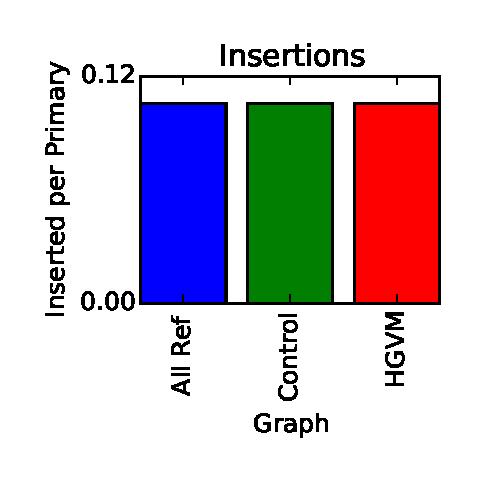
\includegraphics[width=0.4\linewidth]{figures/05_hgvm/mole-insertions.eps}
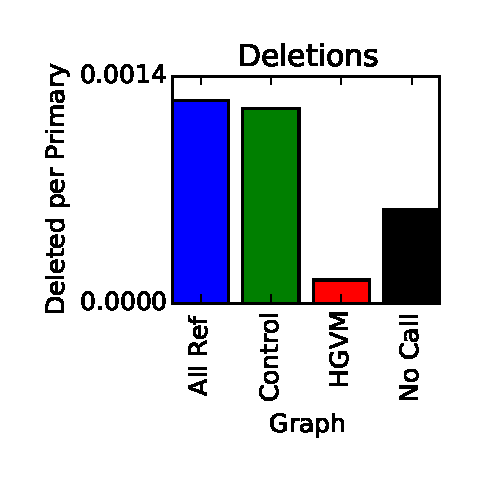
\includegraphics[width=0.4\linewidth]{figures/05_hgvm/mole-deletions.eps}
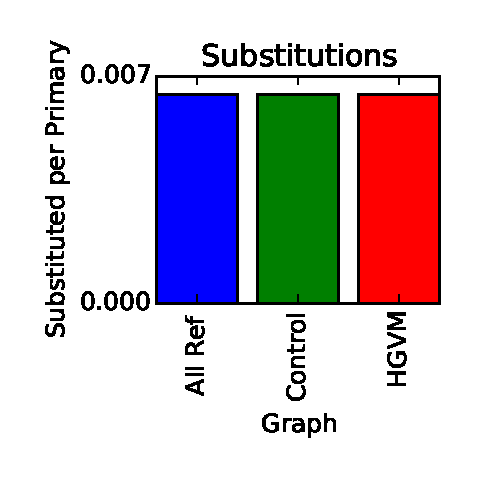
\includegraphics[width=0.4\linewidth]{figures/05_hgvm/mole-substitutions.eps}
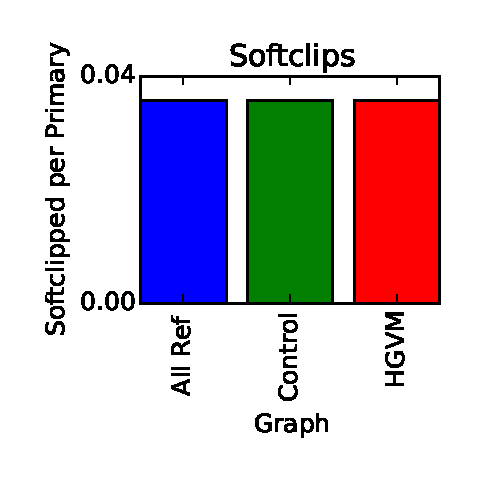
\includegraphics[width=0.4\linewidth]{figures/05_hgvm/mole-softclips.eps}
\caption[Mole realignment evaluation]{Bases involved in events required to align fragments of the CHM1 and CHM13 haploid assemblies to the sample graph created with the \vg variant caller for the combined synthetic diploid sample. Quantities are expressed as bases involved in each type of event per primary path base in the control graph. For the ``All Ref'' condition (blue), the performance of the primary-reference-only control graph as a sample graph was evaluated. For the ``Control'' condition (green), that reference-only graph was used as a reference for variant calling, and the resulting sample graph was evaluated. For the ``HGVM'' condition (red), the Human Genome Variation Map graph under test was used as a reference for variant calling, and the resulting sample graph was evaluated. Finally, for the ``No Call'' condition (black), the Human Genome Variation Map graph was evaluated directly as a sample graph, with no calling step, to serve as a positive control.}
\label{fig:molerealignment}
\end{figure}
% TODO: make a table of this?

\subsection{Structural Variant Evaluation}
\label{subsec:structuralvarianteval}

For the second, VCF-based evaluation, the precision statistics for the five samples analyzed (HG00513, HG00732, NA12878, NA12887, and NA12890) are visible in Table~\ref{tbl:svprecision}, while the recall results for the samples are visible in Table~\ref{tbl:svrecall}.
Summing across samples, the overall precision was~18~out of~25, or 0.72, while the overall recall was~106~of~151, or~0.702, was observed. Together, these produce an F1 score of 0.71.

\newcommand{\true}{\textbullet}
\newcommand{\false}{}

% TODO: This is before the vg add fix and needs to be replaced with the run from 2017-05-09
\begin{sidewaystable}[p]
\centering
\begin{tabular} {l|c|c|c|c|c|c|c}
\textbf{Sample} & \textbf{Position} & \textbf{Type} & \textbf{Length (bp)} & \textbf{1KG SV Call} & \textbf{In dbSNP} & \textbf{In Reads} & \textbf{Verdict} \\
\hline
HG00513 & 17224418 & Insertion & 310 & \true & \false & \true & \true \\
HG00513 & 41552580 & Insertion & 40 & \false & \true & \true & \true \\
HG00513 & 42119316 & Deletion & 28 & \false & \true & \true & \true \\
HG00513 & 19175892 & Insertion & 34 & \false & \true & \true & \true \\
HG00513 & 48754372 & Deletion & 28 & \false & \true & \true & \true \\
HG00732 & 17801132 & Deletion & 322 & \true & \false & \true & \true \\
HG00732 & 40652370 & Insertion & 37 & \false & \true & \true & \true \\
HG00732 & 20360593 & Deletion & 27 & \false & \false & \false & \false \\
HG00732 & 24194512 & Deletion & 5944 & \false & \false & \false & \false \\
HG00732 & 16487502 & Deletion & 35 & \false & \false & \true & \true \\
NA12878 & 43469479 & Insertion & 32 & \false & \true & \true & \true \\
NA12878 & 33391076 & Deletion & 938 & \false & \false & \false & \false \\
NA12878 & 44127743 & Deletion & 48 & \false & \true & \true & \true \\
NA12878 & 17419709 & Insertion & 25 & \false & \true & \true & \true \\
NA12878 & 30430840 & Deletion & 10963 & \false & \false & \false & \false \\
NA12889 & 50234341 & Insertion & 27 & \false & \true & \true & \true \\
NA12889 & 49313687 & Deletion & 3557 & \false & \false & \false & \false \\
NA12887 & 49274738 & Deletion & 26 & \false & \true & \true & \true \\
NA12887 & 43108693 & Deletion & 5907 & \false & \false & \false & \false \\
NA12887 & 49713385 & Deletion & 39 & \false & \true & \true & \true \\
NA12890 & 40398221 & Deletion & 1019 & \true & \false & \true & \true \\
NA12890 & 26495553 & Deletion & 136 & \true & \false & \true & \true \\
NA12890 & 44140033 & Insertion & 31 & \false & \true & \true & \true \\
NA12890 & 26998126 & Deletion & 25 & \false & \true & \true & \true \\
NA12890 & 35628100 & Deletion & 2800 & \false & \false & \false & \false \\ % There are some nearby softclips and what might be a drop in coverage, but not at quite the right places
\end{tabular}
\caption[Structural variant precision]{Precision estimation from 25 randomly-sampled calls of variants inducing length changes of 25~bp or more on chromosome~22. From each sample, five called variants were selected randomly. Variants were manually assessed for corespondence to calls for their sample from the 1000 Genomes structural variant set, correspondence to variants in dbSNP 147, and support in the original GRCh38-aligned input reads, using the UCSC Genome Browser. Variants supported either by the 1000 Genomes truth set or by the reads were designated as true variants, while other variants were designated as false variants. Overall, 18~of 25~variants examined were designated as true, producing a precision estimate of 0.72.}
\label{tbl:svprecision}
\end{sidewaystable}

\begin{table}[p]
\centering
\begin{tabular} {l|c|c|c|c|c}
\textbf{Sample} & \textbf{Total SVs} & \textbf{Called SVs} & \textbf{Recall} \\
\hline
HG00513 & 29 & 19 & 0.66 \\
HG00732 & 31 & 20 & 0.65 \\
NA12878 & 30 & 21 & 0.70 \\
NA12889 & 29 & 21 & 0.72 \\
NA12890 & 32 & 25 & 0.78
\end{tabular}
\caption[Structural variant recall]{Recall statistics for structural variants called by \vg in five samples, with the structural variant VCF used to construct the graph used as the truth set. Overall recall was~106~of~151~variants, or~0.702.}
\label{tbl:svrecall}
\end{table}

\section{Conclusion}

The results of the assembly realignment evaluation show that the graph built in this study is a superior reference for chromosome 22 compared to the primary, linear reference currently in use today, for the purpose of variant calling with the \vg toolkit. In terms of the inserted, deleted, and substituted bases required to represent the CHM1 and CHM13 assemblies on the sample graph called for the synthetic diploid, the variation-containing graph is clearly superior, producing sample graphs that are more similar to the assemblies, and amplifying the effectiveness of the variant caller. However, as evidenced by the overall insert frequency of about 1\% of primary reference bases (Fig. \ref{fig:molerealignment}), and by the relatively low overall structural variant F1 score of 0.71, the \vg variant caller is, overall, still not particularly good.

On the one hand, the \vg variant caller is capable of feats which ordinary pileup-based callers cannot accomplish. For example, at \texttt{chr22:17224418} in HG00513, the \vg caller successfully used short read data to detect a 310~bp insertion, which the 1000 Genomes structural variation data set identifies as an ALU insertion \cite{sudmant2015integrated}. The use of a graph that already contains the ALU insertion in question allows the insertion to be detected using the \vg caller's simple pileup-based approach, whereas ordinarily the detection of such an event would require sophisticated techniques to handle split or discordantly-paired reads or perform local reassembly \cite{wildschutte2015discovery}. This clearly illustrates the power of the graph-based approach.

% TODO: We should talk about the caller design in the methods since that's sort of the method.

However, on the other hand, the \vg caller, being a simple pileup-based caller operating on a few manually-tuned heuristics, makes embarassing mistakes. Take for example the deletion that the caller asserts in NA12878 at \texttt{chr22:30430840}, where the caller asserts a heterozygous deletion of 10,963~base pairs. Nothing of the sort is visible in that region in the genome browser. Indeed, given the allelic depths that the caller computes on that particular allele (51~for the reference and 23~for the deletion), in comparison to the baseline coverage estimate it computes of 38~for the sample, it seems likely that in this case the caller has somehow been fooled by some additional extraneous reads supporting the deletion. Cases like this came up in testing, and some heuristics to reject calls with excessive depth were added to the caller, but there is clearly more work to be done in improving the caller's resilience to this failure mode.

Moreover, if the caller had a more clever architecture (perhaps, like Freebayes~\cite{garrison2012haplotype}, something based on a concept of per-read support for local haplotypes, instead of on pielups), it could potentially be more robust to these failure modes. As it is, it uses poorly-justified heuristics to try and reduce all of the reads aligned to that 10,963-bp potentially-deleted region down to just forward- and reverse-strand ``support'' values, which it compares agains the ``support'' values of the deleted allele in order to attempt to guess the copy number of each. A more robust read-based framework would potentially allow the caller to distinguish misaligned, contaminant, or supernumerary reads, and to somehow discount their support, ultimately resulting in better calls, or at least less embarassing mistakes.

In addition to future improvements to the caller, there are also future improvements that should be made to this study's analytical methods. For example, one shortcoming of the structural variant analysis is that, of the broad diversity available in the 1000 Genomes data set, the five samples analyzed here consistyed of three CEU individuals, one CHS individual, and one PUR individual. These individuals were selected because they were included in the 1000 Genomes structural variation study, and also had high-coverage short-read data aligned to GRCh38 readily available for download. Additional individuals also meeting these criteria likely could have been added to the analysis. To truly evaluate the graph reference constructed in this study, a broader panel of test subjects is needed.

Another reason to test a broader panel of subjects is to avoid overfitting of caller parameters. This study, working only with the five structural variant samples and the one synthetic diploid, had no formal separation between training, test, and validation sets. It is possible that even the relatively low performance of the structural variant caller is overfit, and that it will be reduced when analysis is expanded to more samples. Additionally, the samples used to evaluate the caller were not removed from the input data sets, so it is possible that the presence of variants private to these individuals in the graph artificially inflates the measured performance, relative to what it would be on a genuinely new sample. On the flip side, future studies with a formal separation of training, test, and validation samples might benefit from automatic, machine-learning-based tuning of the numerous configurable heuristics available in the variant caller use dhere, or that will be available in a newly-designed variant caller. In the present study, the heuristics and parameters were hand-tuned, and are almost certainly not optimal.

Overall, the results of this study indicate that graph-based references can be used at chromosome scale to improve variant calling performance. They show that it is possible to combine variation information from disparate sources (in this case, the GRCh38 alternate loci, the 1000 Genomes point variation data set, and the 1000 Genomes structural variation data set) to produce a working graph reference. They show, given the construction runtimes and resource requirements achieved at this scale, that it would not be impractical to construct and evaluate a whole-genome graph reference using these techniques. However, they also show that, in order to use such a whole-genome graph effectively, more research into graph-based variant calling is needed, with a particular focus on porting proven, state-of-the-art read- and read-pair-backed approaches to the graph context.

% TODO: harmonize terminology with the perspective paper. 

\section{Availability of Materials}

The \texttt{hgvm-builder} software, used to coordinate the construction and analysis of the graphs presented here, is available from \url{https://github.com/BD2KGenomics/hgvm-builder}. The constructed chromosome 22 Human Genome Variation Map graph, along with its succinct structural index and substring search indices, is available from \url{http://hgwdev.soe.ucsc.edu/~anovak/outbox/builds/2017-05-09/hgvm/}. This particular graph build has been assigned a UUID of \texttt{aac84e78-3127-4f0c-ac00-a7e488a1802b} by the \texttt{hgvm-builder} software.

\section{Acknowledgements}

The author would like to thank Joel Armstrong for performing Cactus alignments used in this work. The author would also like to thank Charles Markello for preparing flat structural variant VCF files and for contributing to the useful \texttt{toil-vg} library. The author would like to thank Glenn Hickey for preparing the synthetic diploid sample used in the evaluations, for creating the \texttt{hal2vg} tool, and also for contributing to \texttt{toil-vg}. The author would like to thank Mike Lin for creating the \texttt{vg\_docker} system used to package \vg for this study.

% Towards a Human Genome Variation Map
    % Intro
        % So in the bake-off paper, aka last chapter, we showed that it's possible to get improved variant calling performance with a graph reference
        % But we had these references with only short variants in them that did really well
        % Can we improve performance by bringing in more info about long variants and alt loci?
    % Methods
        % We developed a method to add variants from a VCF into a graph
            % It's based on all these realignment heuristics to try and get good performance/not crash
        % We also improve the assembly realignment evaluation from the paper
            % By not going through VCF and instead infering presence/absence of nodes and edges from nested, ploidy-aware genotype calls
        % We developed an HGVM building and evaluating tool which is here on Github/pip
    % Results (still preliminary)
        % We built a graph for chr22 on 3/23/17
        
            % TMPDIR=/hive/users/anovak/tmp time build-hgvm ./tree2 chr22_build --base_vg_url file:`pwd`/sourceGraphs/human22.only.chopped.vg --vcf_contig "chr22" --vcfs_url file:`pwd`/../forward_vcfs --vcfs_url file:/cluster/home/charles/SV_HGVM_research/eighth_draft_GRCh38_bks_only_polALengths_chrs --add_chr --sample_fastq_url file:`pwd`/../mole_bams/syndip-chr22-fastq.R1.fastq --sample_fastq_url file:`pwd`/../mole_bams/syndip-chr22-fastq.R2.fastq --eval_sequences_url file:`pwd`/to_realign.seqs --dump_hgvm ./chr22_build_dump --logInfo --realTimeLogging | tee log.txt
            
        % On chr22 (chr21?) we see improved variant calling performance, as measured by the realignment eval, between calling on the graph and calling on a linear control graph
            % If time permits, we can do a leave-one-out on the data sources and see if they all contribute positively
        % On chr22 (chr21?) we see improved SV calling performance, as measured by recall against the 1kg VCF for NA12878, relative to calling against a linear control
            % TODO: implement that linear control
            % Again, we can try controls from other subsets of the input data (just alts, just 1kg point variants, etc.)
                % And we can move the "what's an SV" threshold around to exclude the point variants if there's crosstalk
        % For the whole genome, here is a cool way (IPFS? DAT?) to retrieve a graph build with index
    % Conclusions
        % We are indeed barking up the right tree with graph-based references
        % More work is needed
            % To validate the whole genome build
            % To pull in more data
            % To polish the tools
            % To establish best practices



% %%%%%%%%%%%%%%%%%%%%%%%%%%%%%%%%%%%%%%%%%%%%%%%%%%%%%%%%%
% bibliography

% 2010june01 sol katzman:
% if \nocite is specified, all entries in the bib file are included,
% probably not what you want, so comment out the \nocite and only get the cited references.
%\nocite{*}

% 2010june01 sol katzman:
% this makes the bibliography single spaced, with double spacing between entries
\def\baselinestretch{1.0}\large\normalsize

% We need this for natbib for some reason
\def\newblock{\hskip .11em plus .33em minus .07em}
\bibliographystyle{plainnat}
\bibliography{thesis}

\end{document}
